%%%%%%%%%%%%%%%%%%%%%%%%%%%%%%%%%%%%% What students learn %%%%%%%%%%%%%%%%%%%%%%5
\tcbsection{Curriculum, Instruction, and Assessment}
\subsection{B1 What Students Learn Criterion}

{\centering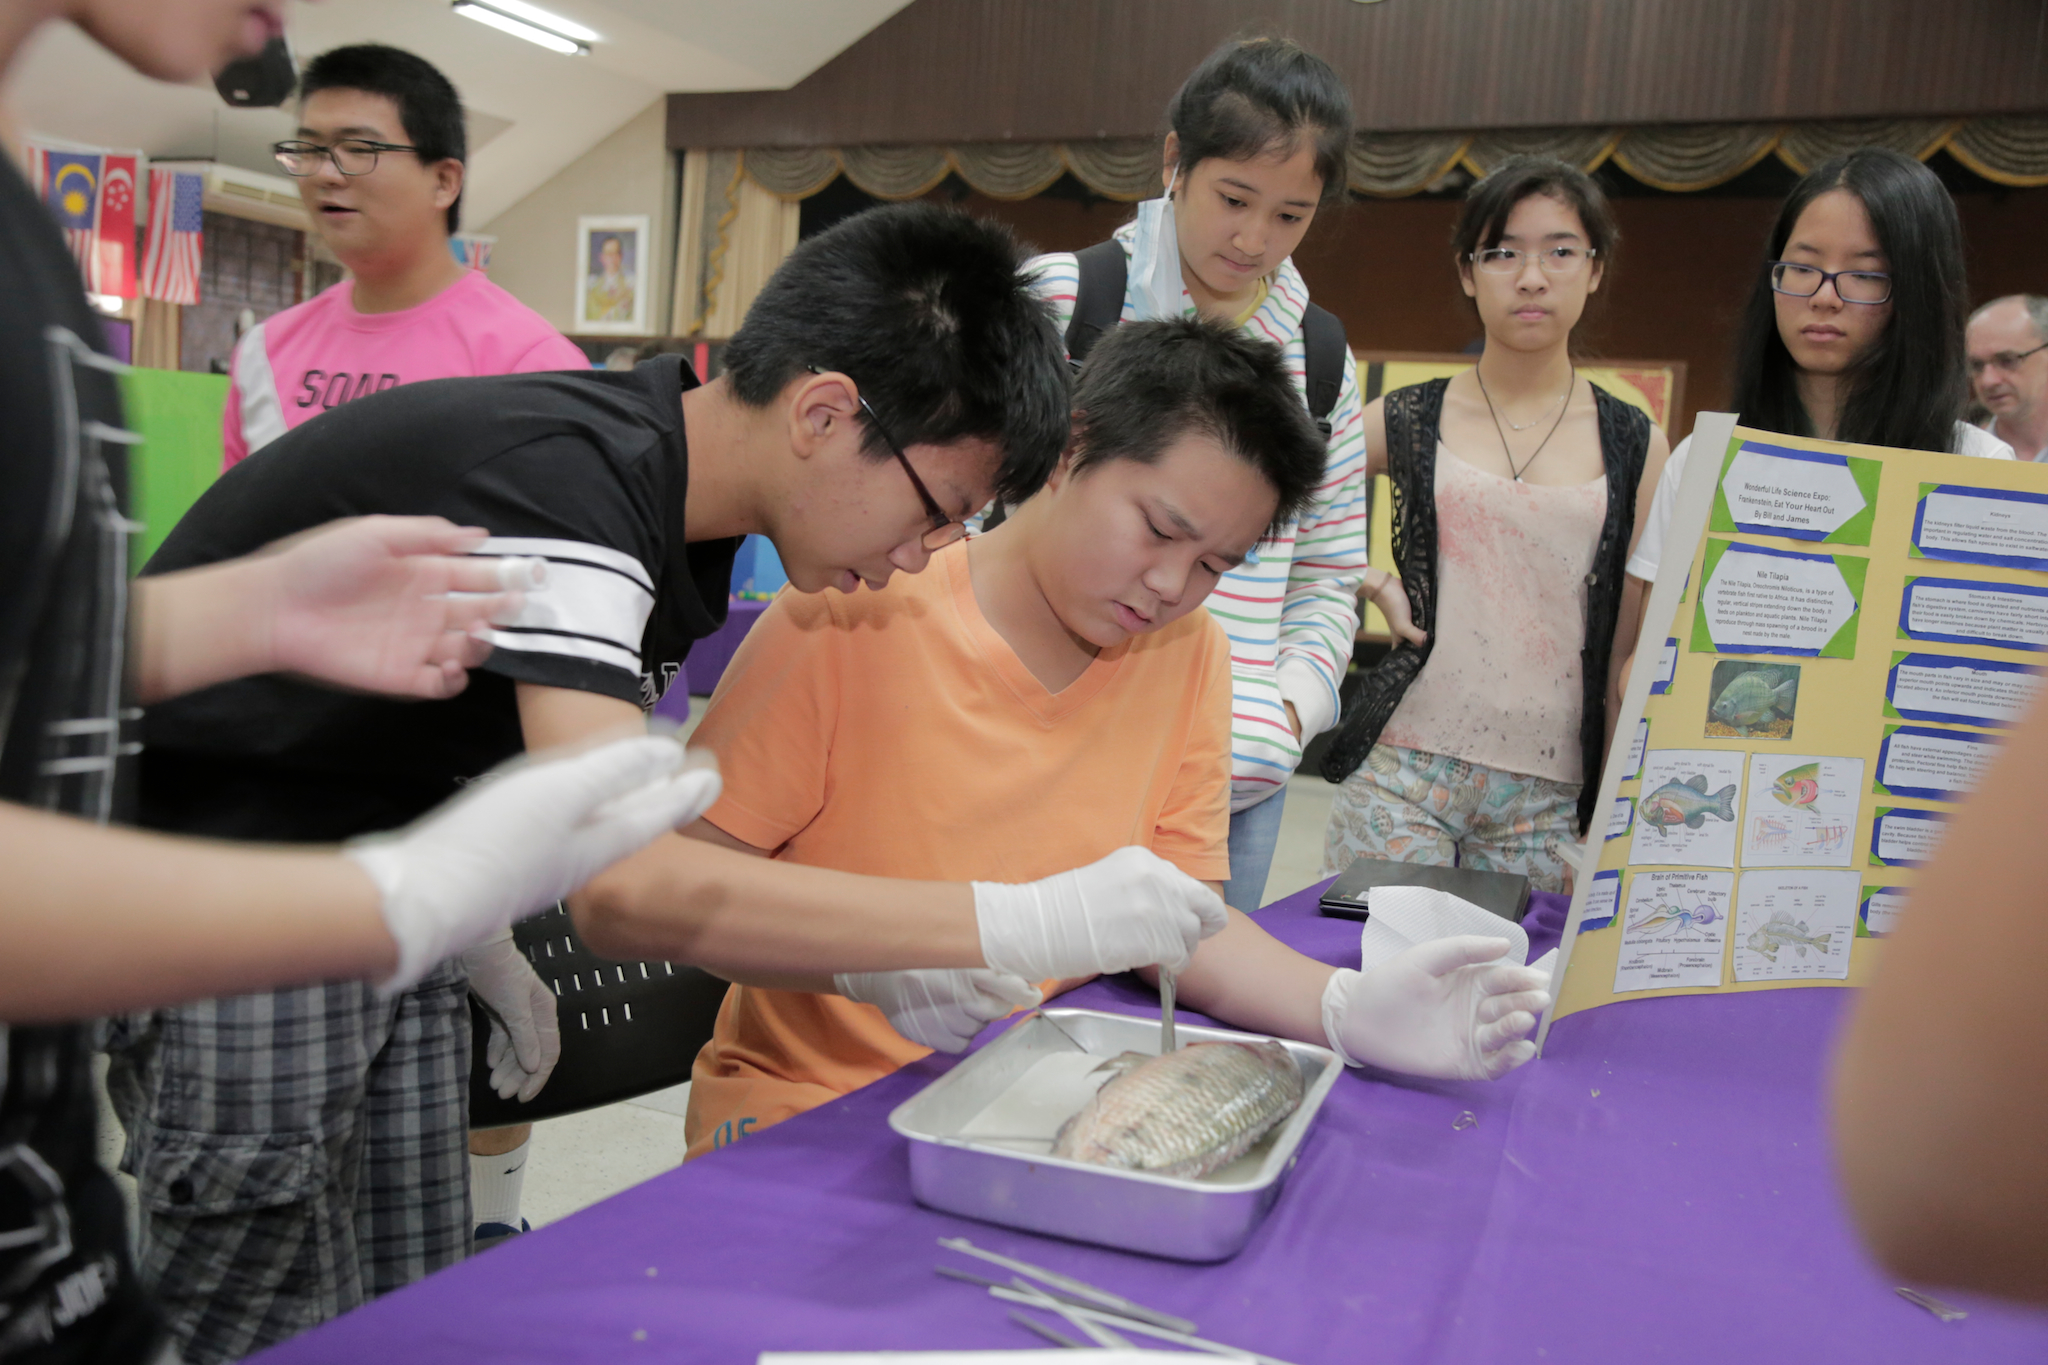
\includegraphics[width=\textwidth]{chapter4_B1_p1.jpg}}

\subsubsection{Current Educational Research and Thinking}
\indicator{The comprehensive and sequential documented curriculum is modified as needed to address current educational research and thinking, other relevant international/national/community issues and the needs of all students.}

\prompt{Comment on the effective use of current educational research related to the curricular areas in order to maintain a viable, meaningful instructional program for students. Examine the effectiveness of how the school staff stay current and relevant and revise the curriculum appropriately within the curricular review cycle.}

\begin{findings}
CMIS Leadership and Teaching Staff continue to address and develop a comprehensive and sequential curriculum. 

\href{https://drive.google.com/drive/folders/0B71_pYxcTLo-NGJ4N0RQWXRTNE0?usp=sharing}{\minor{Standards}}

CMIS Leadership Team strongly believes that at the core of a rigorous, engaging, coherent curriculum are research-based standards. The  CMIS Teaching Staff use multiple, comprehensive, and appropriately sequenced standards that inform and provide the foundation of our curricular decisions (see section entitled, Academic Standards in Each Area). 

{\centering\includegraphics[width=\textwidth]{4_2_1_wl_b.jpg}}

The 2013-2014 academic year saw a great deal of change to the standards which directly impacted and continue to influence curricular decisions. The CMIS Teaching Staff, with the support of the Leadership Team, adopted new standards in ELA, mathematics, and science, as well as finalizing the adoption of all other content standards (i.e., physical education, social studies, health, fine arts, world languages). 

The adoption of these standards, especially in ELA, mathematics, science, and 9-12 history  reflect \href{https://docs.google.com/a/cmis.ac.th/document/d/1XkW4kx-s2f5rP1zWNLqi14WBQ9fHp9aFRP2op2RPRQE/edit?usp=sharing}{significant shifts} in conceptual understanding of the content, have major implications on instruction and assessment, and illuminate real increases in depth of knowledge and rigor. All curricular decisions would have to be made based upon these new realities. Furthermore, CMIS has begun to view our adopted standards as the bedrock of all unit creation and planning. Standards also continue to help guide appropriate instruction and ensure rigor. 

Because of these conceptual shifts, the 2014-2015 saw a strong focus on professional development topics relating to the difference between curriculum and standards, and the shared responsibility of the CMIS Literacy Standards. Teachers, community members, and administrators were involved in multiple discussions and the CMIS Leadership Team believed this was an appropriate starting point for teachers and community members to begin understanding the standards and curriculum. See PTG Curriculum, Professional Development \href{https://drive.google.com/a/cmis.ac.th/folderview?id=0ByVFfrm0zfolWE0yenprdktGVlk&usp=sharing}{Folder} for community presentations. 

\href{https://docs.google.com/a/cmis.ac.th/document/d/1hh1nLUlJgg1hd7s6aG3u3We0L6o7Wg_ECdjc2f6DcT8/edit?usp=sharing}{\minor{Curriculum Review Cycle}}

Since curricular decisions should be made using clear standards and student outcomes as a guide, a new \href{https://docs.google.com/presentation/d/15ZhVBwOO3psFCM44ybsXFUNqrhpHmVHdekAzIXjRJ5U/edit?usp=sharing}{Curriculum Review Cycle/Resource Adoption strategic plan} had to be developed and implemented. The most important elements of the Curriculum Review process are the specific evaluations tools, rubrics, and vetting instruments that have been developed and used to narrow down vendors and products for curricular and resource materials. CMIS Leadership also provides the necessary \href{https://drive.google.com/file/d/0B4n_WCeTYd4_U2J0YnRWYVp4bk0/view?usp=sharing}{time} and \href{https://drive.google.com/file/d/0B4n_WCeTYd4_NjBfVm92blF6T00/view?usp=sharing}{space} required for teacher collaboration in vetting and evaluation of curricular items. 

{\centering\includegraphics[width=\textwidth]{4_2_1_wl_c.jpg}}

Science curriculum was the first content to be vetted and evaluated based upon the Curriculum Review Cycle; science curriculum was purchased during the 2015-2016 school year. As with ELA curriculum decisions, science saw significant conceptual changes with the adoption of the the \href{https://drive.google.com/a/cmis.ac.th/file/d/0B71_pYxcTLo-eUtQZE9DLTFvYUE/view?usp=sharing}{Next Generation Science Standards}. Because of this, CMIS Leadership, developed \href{https://docs.google.com/a/cmis.ac.th/document/d/1u0crwv2uVJdfamGYP9NYsUvub7bkPO64dIu0uAAkSIo/edit?usp=sharing}{vetting and evaluation instruments} to ensure curriculum and resource alignment with the standards, as well as rigor and student engagement. This year, mathematics undertook the same curriculum vetting process and ELA/social studies will be reviewed next year. 

In order to ensure that the resources we purchase outside of the normal adoption cycle are of the highest quality and they meet our three general criteria of: is it aligned to the standards? Is it rigorous? and is it engaging? \href{https://goo.gl/forms/715q4GLbzFj9JRPZ2}{Resource Request} and \href{https://goo.gl/forms/N2Oow0UnpUr7bOzw1}{Resource Renewal} forms were developed and implemented. 

{\centering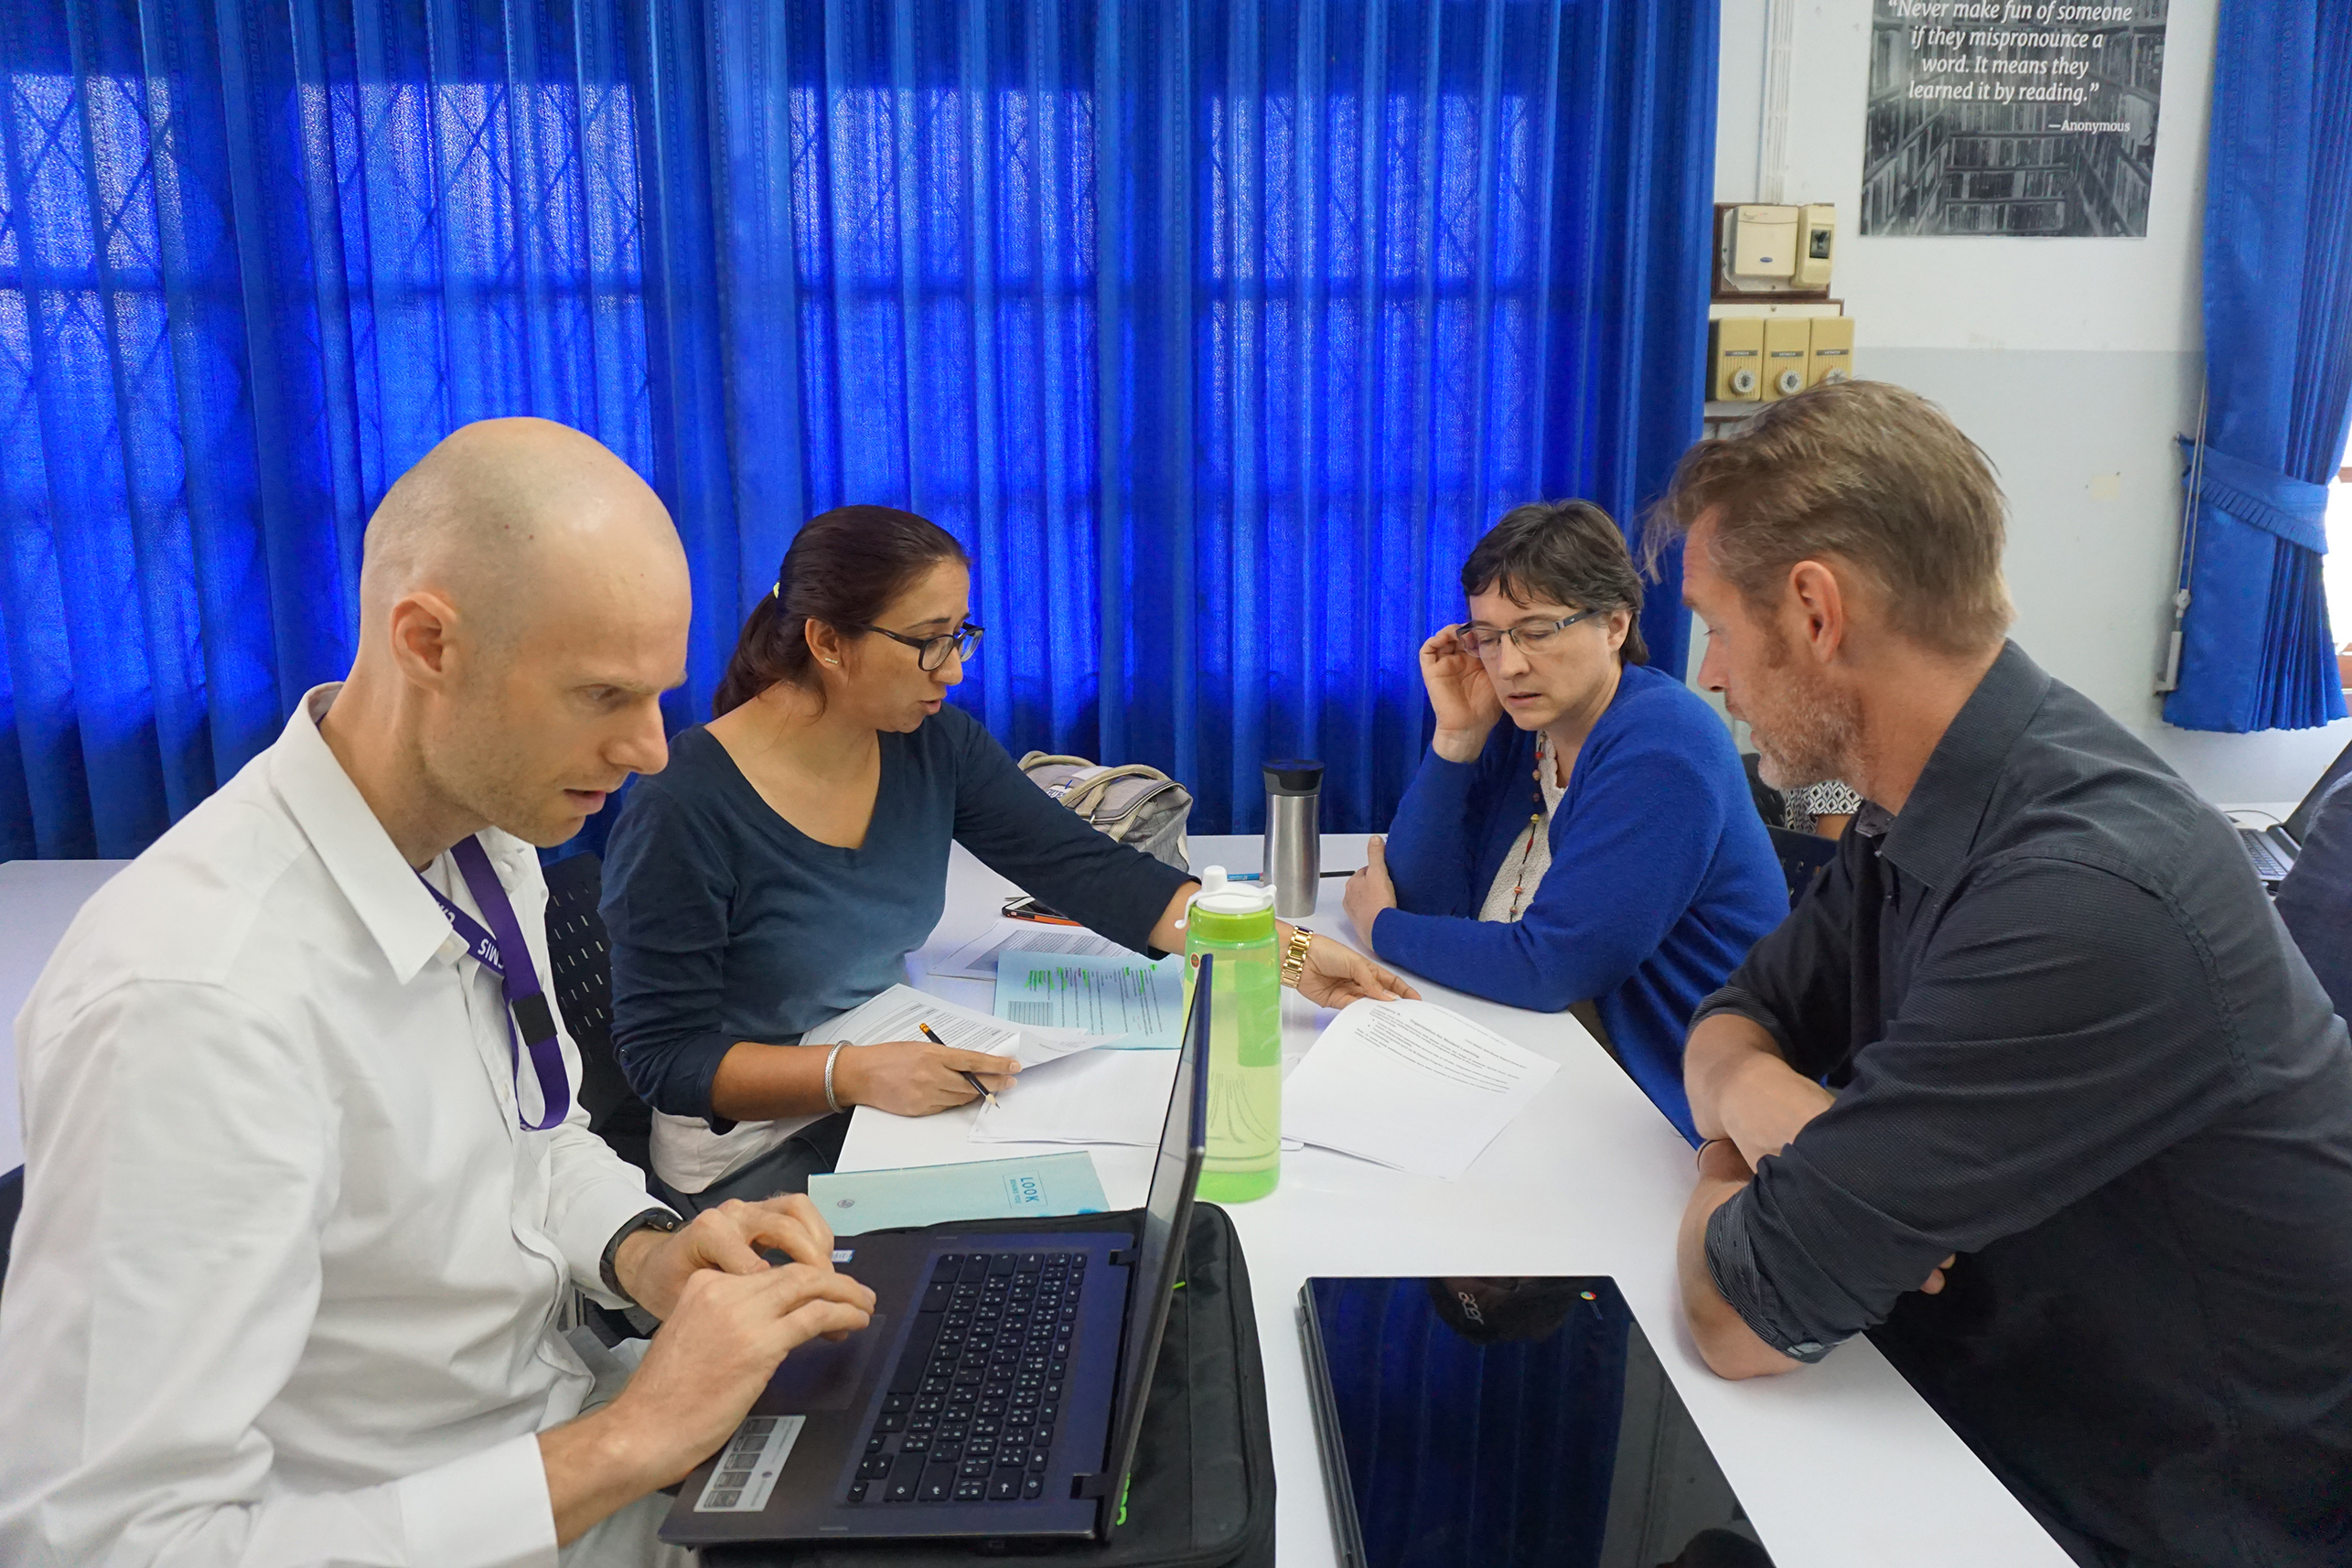
\includegraphics[width=\textwidth]{chapter4_B1_p2.JPG}}

\minor{Understanding by Design Units}

The past two years have also focused on the research-based planning tool Understanding by Design (UbD) as the primary framework for unit/curriculum development. A group of teachers attended a UbD workshop March 2014 and were encouraged by the process. In October, 2014, CMIS was fortunate to have UbD consultant Elizabeth Rossini provide a \href{https://drive.google.com/drive/folders/0ByVFfrm0zfolbDlqWjhobkhDZkk?usp=sharing}{two-day, 15 hour professional development workshop} on UbD essentials. Subsequent mini workshops have also been provided in targeted areas of UbD development; both expert teachers and the CMIS Leadership Team have been involved in the development and delivery. Teachers are required to develop and submit at least two UbD units per year, with some departments requiring more. The UbD units for 2015-2016 have reflected the prior year’s professional development focus. In that, they have been central to ensuring that the literacy shifts and standard alignment have been met. CMIS Leadership Team believe strongly in applying our professional development focus in everyday instruction and assessment; CMIS UbD units are one way to achieve this. Please see UbD Units folder for \href{https://drive.google.com/drive/folders/0ByVFfrm0zfolQkFTQjNQMDhBN1E?usp=sharing}{2014-2015}, \href{https://drive.google.com/drive/folders/0ByVFfrm0zfolfl9RaFBtSy1YLVM2LUJONGNVcDAxbTZIWTNKTXVFZnh6eEUybjIwQi1RR3M?usp=sharing}{2015-2016}, \href{https://drive.google.com/drive/folders/0ByVFfrm0zfolak8xTjQ3NVhCbmc?usp=sharing}{2016-2017} and UbD \href{https://drive.google.com/a/cmis.ac.th/folderview?id=0ByVFfrm0zfolfmUyZV9DbGoxZVhpVHpGdG9MeEt6MHZJaEtoT3VzTjM0bkk5NFQ5MVJldUU&usp=sharing}{Resources}, UbD \href{https://drive.google.com/drive/folders/0ByVFfrm0zfolcXpjOUJTSmdIT1k?usp=sharing}{Resource In House}, UbD \href{https://docs.google.com/a/cmis.ac.th/document/d/1kL1VjwfuMMa7NaWmwUrEah1BM-jJRmLAd4VJzR3HoPs/edit?usp=sharing}{Master List}, and UbD \href{https://docs.google.com/a/cmis.ac.th/document/d/11IXUy-YcnFG8dMzr42iBigOuh1GmLVjcu_Ulv19r9Yg/edit?usp=sharing}{Checklist}. 

The CMIS Google Drive is the primary method of organizing and archiving  of the curricular units. The Drive along with the the \href{http://www.cmis.ac.th/}{CMIS Teacher Dashboard}, found on the school website, is a place where teachers can access these resources. The Dashboard also contains the \href{https://drive.google.com/drive/folders/0ByVFfrm0zfolfmV1QTNuWFdUVHV3dDVrRFMzUFBMazY0VGs1eWc0cmFjVGcwNDdsQkdrZzA?usp=sharing}{CMIS Standards Blueprints}. Teacher feedback and anecdotal evidence suggested that greater alignment of the UbD units to the standards would be possible if the teachers had a general blueprint or pacing guide to help them visualize and map the whole year of standards. Department and grade level teams began the blueprint work at the beginning of the 2015-2016 year. All core subjects, with the exception of K-5 ELA and mathematics, have been completed. 

\minor{Scope and Sequencing-Standard \href{https://drive.google.com/drive/folders/0ByVFfrm0zfolfmV1QTNuWFdUVHV3dDVrRFMzUFBMazY0VGs1eWc0cmFjVGcwNDdsQkdrZzA?usp=sharing}{Blueprints} }

ELA blueprints posed a challenge as standards are addressed all year long. In order to address this challenge, small groups were scheduled for focused professional development using the Partnership for Assessment of Readiness for College and Careers ELA Model Frameworks (PARCC, 2016) . Collaboration time was given to ELA teachers in grades 6-12 to complete this work. 

\minor{So what...}

The combined teamwork of all stakeholders: the CMIS Leadership Team, the community, outside research, vetted educational organizations, and, most importantly,  the teachers themselves, ensure that CMIS staff at all levels stay current in educational research. Though CMIS ensures we stay current, there are questions about whether the current research in standards, understanding by design, and researched based resources transfers to actual classroom instruction. 
\end{findings}

\subsubsection{Academic Standards for Each Area}

\indicator{The school provides a comprehensive and sequential documented curriculum that is articulated within and across grade levels for the improvement of programs, learning, and teaching.}

\prompt{ Evaluate to what extent there are defined academic standards for each subject area, course, and/or program (e.g., online instruction) that meet state or national/international standards.}

\begin{findings}
CMIS is in the process of developing a comprehensive and sequentially  documented curriculum that is articulated within and across grade levels by combining vetted resources, research-based standards, sound pedagogical practices, and addressing fidelity to the adopted standards. 

Though it is a work in progress, many elements that make up a coherent curriculum are beginning to take place, this includes  quality resources, structured, teacher-developed units, and research-based standards.   

\minor{\href{https://drive.google.com/drive/folders/0B71_pYxcTLo-NGJ4N0RQWXRTNE0?usp=sharing}{CMIS Academic Standards}}

CMIS Leadership and Teaching Staff strongly believe in the importance of the school’s academic standards. CMIS Staff use a common understanding of academic standards: 

Academic standards define the concepts, skills, and knowledge that students should know and be able to do in each curricular area, the level at which students are expected to demonstrate this knowledge, and grade-level expectations for performance. In a standards-based educational system, schools determine the benchmarks for student work that meet these standards, provide appropriate instruction, and use multiple assessment measures to identify the level of achievement for all students. This approach assists the schools in defining the quality accomplishment of the complementary schoolwide learner outcomes and the degree to which all students are achieving them. Standards do not describe any particular teaching practice, curriculum, or assessment method (\href{https://docs.google.com/a/cmis.ac.th/document/d/1ApZ_fARdmcK_9fEeb8uoWyGa50572P8z-sM9JeTQygQ/edit?usp=sharing}{Abbot, 2013})

\minor{CMIS Standards} 

\begin{itemize}
\item Common Core State Standards \href{https://drive.google.com/a/cmis.ac.th/file/d/0B71_pYxcTLo-Y1FGYl9JeUotbXc/view?usp=sharing}{ELA} (Reading, Writing, Foundational Skills, Language, Speaking and Listening)*
\item Common Core State Standards \href{https://drive.google.com/drive/folders/0B71_pYxcTLo-MkJPLU5tQk1ySWM?usp=sharing}{Mathematics}
\item \href{https://drive.google.com/drive/folders/0ByVFfrm0zfolN01lX0hnejZ4Q0U?usp=sharing}{Next Generation Science Standards} (NGSS)*
\item \href{https://drive.google.com/drive/folders/0ByVFfrm0zfolMjlnc0JtcVRVYjA?usp=sharing}{AERO Standards} (aligned to \href{http://www.socialstudies.org/standards/strands}{NCSS framework}) grades K-8*
\item National Standards for History (from UCLA) grades 9-12 (\href{http://www.nchs.ucla.edu/history-standards/world-history-content-standards}{World} and \href{http://www.nchs.ucla.edu/history-standards/us-history-content-standards}{US})
\item \href{https://drive.google.com/a/cmis.ac.th/file/d/0ByVFfrm0zfolbG9hN21kR2FXZVU/view?usp=sharing}{C3 Framework} (piloted 2016-2017)*
\item \href{https://drive.google.com/drive/folders/0B71_pYxcTLo-NDhTcTJLQU82WVU?usp=sharing}{National Coalition for Core Arts Standards} (music, art, theater)  (NCCAS)
\item \href{https://drive.google.com/a/cmis.ac.th/file/d/0B71_pYxcTLo-U1BYR3JXMUZhUW8/view?usp=sharing}{Computer Science Teachers Association Framework} (CSTA)
\item \href{https://drive.google.com/a/cmis.ac.th/file/d/0ByVFfrm0zfolakw5TUstQ1ZrVDFCRjR1d1JQSUpQbkZaVDBr/view?usp=sharing}{ISTE for Students and Teachers} (ISTE)
\item \href{https://www.iste.org/standards/standards/standards-for-administrators}{ISTE for Administrators} 
\item \href{https://drive.google.com/drive/folders/0ByVFfrm0zfolfk9CLWctcnk2RlJYX1RaWGpkZktWRTR2MVQ5aEQ0SGg0R280VGV5Tm81bm8?usp=sharing}{World Readiness Standards for Learning Languages}
\item \href{https://drive.google.com/a/cmis.ac.th/file/d/0ByVFfrm0zfolOE8wcTR5Y19BZms/view?usp=sharing}{Physical Education Model Content Standards} for California Public Schools 
\item \href{https://drive.google.com/drive/folders/0ByVFfrm0zfolfmJGZ3B1anNJc0hNTTZobHlKMXBFbTlDQUVvMXNQQVhUWklocUd0VGY3eTg?usp=sharing}{National Health Education Standards} (Center for Disease Control)
\item \href{https://drive.google.com/a/cmis.ac.th/file/d/0ByVFfrm0zfolM0VpbFNHNXlfbGs/view?usp=sharing}{Standards for the 21st Century Learner} (American Association of School Librarians)
\item \href{https://drive.google.com/a/cmis.ac.th/file/d/0ByVFfrm0zfolMTU1cXlocHR0dGs/view?usp=sharing}{Wisconsin’s Model Academic Standards for Business}  
\item AP Course Topics and Indicators  (Overviews)
\end{itemize}
* standards are internationally benchmarked 

Research indicates CCSS (both ELA and Mathematics), NGSS, C3, and NCCAS are standards that are considered rigorous, world class, and allow for deeper engagement around fewer concepts/topics.

\minor{Sound Pedagogical Practices}
 
In order to address the prior visiting team’s 2011 observation that some teachers did not feel that they understood the standards or ``little understanding of the 'next steps' needed to unpack the standards'', CMIS has provided professional development for the CCSS ELA, NGSS, and CCSS Mathematics. Starting from the critical conceptual shift found in the CCSS that literacy is a ``shared responsibility'' of ALL staff, K-12, all contents, the CMIS Leadership Team devoted a majority of 2014-2015 to unpacking and analyzing the newly adopted ELA standards with the whole staff.  Since ALL teachers have literacy standards, the professional development ensured that teachers not only focused on their own grade-level standards (i.e ``...within the grade level''), but also worked with the anchor standards that addressed vertical progression of outcomes (i.e. ``...across grade levels''). See Action Plan Curriculum and Instruction 2014-2017 for more information on professional development at CMIS.

\minor{Fidelity to Standards}

Depending on the grade level, division, and/or department; \href{https://docs.google.com/a/cmis.ac.th/document/d/1kL1VjwfuMMa7NaWmwUrEah1BM-jJRmLAd4VJzR3HoPs/edit?usp=sharing}{UbD plans}, mid/end of year assessment, peer reflection, and administrative observational walkthroughs are all methods to ensure instructional fidelity to the standards. 

{\centering\includegraphics[width=\textwidth]{4_2_1_wl_d.jpg}}

\href{https://drive.google.com/drive/folders/0ByVFfrm0zfolfmV1QTNuWFdUVHV3dDVrRFMzUFBMazY0VGs1eWc0cmFjVGcwNDdsQkdrZzA?usp=sharing}{Course and grade level blueprints} have also been developed to use as a guide for vertical and horizontal integration discussion and collaboration to determine if modification is necessary. Areas that have been discussed are standards overlap and skill/content gaps. 

\minor{Vetted Instructional Resources}

As mentioned earlier, CMIS Leadership Team believe that all curricular decisions should be based on three basic questions: is it aligned to the standards, is it rigorous, and is it engaging? During the 2015-2016 school year, the CMIS Middle and High School Science department, representative teachers from K-5, and CMIS Leadership Team vetted and evaluated science materials using \href{https://docs.google.com/a/cmis.ac.th/document/d/1u0crwv2uVJdfamGYP9NYsUvub7bkPO64dIu0uAAkSIo/edit?usp=sharing}{CMIS developed rubrics} and instruments based upon \href{https://drive.google.com/a/cmis.ac.th/file/d/0ByVFfrm0zfolWmtFbld4MExkdGc/view?usp=sharing}{EQuIP} (Educators Evaluating the Quality of Instructional Products) Rubric. The outcome was the purchase of \href{https://drive.google.com/drive/folders/0ByVFfrm0zfolVERNZUJiX2pYNjA?usp=sharing}{FOSS Kit science materials} that met and exceeded our criteria for grades K-5. FOSS Kits for science have been purchased and CMIS will continue to provide time and assistance to help teachers utilize and implement this curriculum resource. 

During the 2016-2017 school year, mathematics curriculum was reviewed and and resources were vetted. Through the use of \href{https://drive.google.com/drive/folders/0ByVFfrm0zfolWHVZRlNuYWppWGM?usp=sharing}{Instructional Materials Evaluation Tool} (IMET), developed by Achieve the Core, the K-5 group adopted two resources that aligned strongly with the standards and the instructional shifts in mathematics (Focus, Coherence, and Rigor). The first resource from Great Minds Inc. is entitled Eureka Math. \href{https://greatminds.org/math}{Eureka Math} not only aligns with the standards, it provides appropriate coherence, focus, and rigor. The second resource vetted and purchased was \href{http://help.k12.mhedu.com/connected/}{My Math} published by McGraw Hill. Again, the adoption committee  found good alignment to the standards and the instructional shifts. Both programs provide a balance of rigor- application and conceptual knowledge in Eureka and procedural skills in My Math. 

Curricular decisions are also made as a result of our professional development.  After CMIS workshops on the CCSS conceptual shifts and with discussions with teachers, it was determined that the school lacked appropriately complex informational text in grades 9-12. Because of this discovery, plans and funds were set aside to purchase informational text. For example, the science department ordered class sets of the informational text, Stuff Matters and the English/Language Arts department ordered informational titles such as Hiroshima, I Am Malala, and Night. 

AP courses have appropriately rigorous and cognitively challenging key concepts that are addressed throughout the sequence of an AP course.  

\minor{So what...}

CMIS has made great strides in unpacking and analyzing some standards, especially CCSS ELA and mathematics. More time and resources need to be committed to ensure CMIS teachers become experts in all their standards. Also, though having fidelity to the standards and ensuring that the standards are being addressed in instruction is an important first step, more work needs to be committed to creating clear curricular sequencing through multiple grade level blueprinting. 
\end{findings}

\subsubsection{Embedded Global Perspectives}

\indicator{The school leadership and certificated staff ensure that global education concepts, perspectives, and issues are embedded within the curricular areas.}

\prompt{Examine the curricular documentation and observe the delivered curriculum to determine the extent to which there is integration of global concepts, perspectives, and issues.}

\begin{findings}
The CMIS Leadership and Teaching Staff ensure that global education concepts, perspectives, and issues are embedded within the curricular areas.

CMIS Leadership and Teaching Staff wanted to describe evidence that goes beyond the traditional list of events that international schools normally cite for embedding global perspectives. Though CMIS Leadership, teaching staff, and community still organize and implement an \href{https://drive.google.com/drive/folders/0B0TYmzaZNi3fbnhzMzNNT3hKNm8?usp=sharing}{International Day} which rotates with Thai Day (i.e. every other year); other major events events such as \href{https://drive.google.com/drive/folders/0B0TYmzaZNi3fdlJuWDFxb0NpemM?usp=sharing}{Model United Nations} and \href{https://drive.google.com/drive/folders/0B0TYmzaZNi3fUkdpR1hLaDVaekk?usp=sharing}{National History Day} are also scheduled. Each of these events showcase and celebrate our unique place on the globe and our diverse community. There is also evidence of more routine and implicit examples of how CMIS promotes and embeds global perspectives. 

\minor{Internationally Benchmarked Standards}

Most importantly, and generally overlooked, are our adopted standards. Of the core courses (ELA, Mathematics, Social Studies, and Science), all four set of standards are internationally benchmarked. This benchmarking  ensures CMIS students are exposed to global perspectives. As \href{https://docs.google.com/a/cmis.ac.th/document/d/1ApZ_fARdmcK_9fEeb8uoWyGa50572P8z-sM9JeTQygQ/edit?usp=sharing}{Achieve (2014)} states about our adopted ELA and Mathematics standards, 

``As part of the Common Core State Standards Initiative, Achieve helped collect and analyze standards from a number of countries. These studies helped inform the choices made by the writers of the common standards.''

For Next Generation Science Standards, \href{https://docs.google.com/a/cmis.ac.th/document/d/1ApZ_fARdmcK_9fEeb8uoWyGa50572P8z-sM9JeTQygQ/edit?usp=sharing}{Achieve} stated: 

``The overall goal of Achieve’s study on international standards is to inform the development of the NRC framework and Next-Generation Science Standards.''

And finally, \href{https://docs.google.com/a/cmis.ac.th/document/d/1ApZ_fARdmcK_9fEeb8uoWyGa50572P8z-sM9JeTQygQ/edit?usp=sharing}{College, Careers, and Civics Framework (C3)} states: 

``...standards (including C3) suggests that all standards should be rigorous, world class, and internationally benchmarked, while also allowing for deeper engagement around fewer concepts/topics.'' 

CMIS Leadership feel confident that as we remain focused on aligning appropriate standards to our assessments, lessons, and instruction, we can be assured that we are providing standards with a global perspective 

\minor{Staff Diversity}

The diversity of our Leadership Team and Teaching Staff ensure multiple perspectives, concepts, and issues are embedded in CMIS lessons and discussions. Diversity of not only nationality, but age, gender, and experiences makes CMIS a dynamic and engaging global workplace. See \href{https://docs.google.com/a/cmis.ac.th/document/d/1xv5c4vDAjs6UksU69e5l8UEZu0kYYJblDoKUj-29iXE/edit?usp=sharing}{Chapter 1: Student/Community Profile and Supporting Data} for more information on staff diversity. 

\minor{Strategically Adopted Globally Minded Resources}

Finally, resources are adopted, especially text in the library, that provide perspectives on multiple global issues from authors such as Linda Sue Park and Grace Lin. Choices from Brown University and Facing History and Ourselves are globally minded resources that ask students to engage in global minded dispositions such as developing a sense of personal agency and belief in the capacity to affect outcomes in the future. 

\minor{So What...}

CMIS Leadership and Teaching Staff would benefit from taking a more explicit approach to embedding global perspectives in both the curricular,  instructional, and school climate decisions. Student perceptions indicate that a vast majority believe that as they are learning in an “international school”, they are automatically getting global perspectives, as if through osmosis.  CMIS should dedicate time and resources in developing units that address global dispositions and provide student discussion in Communication Groups. 
\end{findings}

\subsubsection{Congruence}

\indicator{There is congruence between the actual concepts and skills taught, the academic standards, and the schoolwide learner outcomes.}

\prompt{Evaluate if there is congruence between the actual concepts and skills taught, the academic standards, and the schoolwide learner outcomes.}

\begin{findings}

CMIS Leadership and teaching staff continue to address congruence between the actual concepts and skills taught, the academic standards, and the schoolwide learner outcomes through a variety of methods. 

\minor{Vetted and Evaluated Resources}

CMIS vets and evaluates adopted resources to ensure alignment to the academic standards. For example, FOSS kits adopted for science and Eureka math adopted for math both have been measured to have strong alignment to the standards and the instructional shifts found within those standards. See section entitled: Academic Standards for Each Area for more information. See adoption resources: Adoption Resources: \href{https://drive.google.com/drive/folders/0ByVFfrm0zfoleXEyU3I0cTBXMVk?usp=sharing}{Science 2015-2016}, \href{https://drive.google.com/drive/folders/0ByVFfrm0zfolakRsUVNBaXhWcjQ?usp=sharing}{Math 2016-2017}, \href{https://drive.google.com/drive/folders/0ByVFfrm0zfolLUN5UThPTG5wQlE?usp=sharing}{AP Human Geography 2016-2017}, \href{https://drive.google.com/drive/folders/0ByVFfrm0zfolfkhGeTFZSVRmSFNEZmhlaWZneEE5T0lwWjNQVnlFYVVWVlljU1RBTDZQc1k?usp=sharing}{World Language 2014-2015} 

\minor{Understanding by Design (UbD)}

The \href{https://docs.google.com/a/cmis.ac.th/document/d/1kL1VjwfuMMa7NaWmwUrEah1BM-jJRmLAd4VJzR3HoPs/edit?usp=sharing}{Understanding by Design} is one of the curricular instruments used to ensure congruence. The UbD design ensures that developers first determine the standards that the unit of instruction will address. The design also asks developers to address what knowledge and skills will be taught during the unit. The CMIS UbD unit goes further than the traditional UbD template by adding a handful of modifications to ensure congruence between our skills/knowledge, our adopted standards, and the SLOs within the unit; see \href{https://docs.google.com/a/cmis.ac.th/document/d/1wwb5O3EmHNmzx7MOdHvi0TFjyYRWyELnyD1VRsmuj1Y/edit?usp=sharing}{Table 1}.  

\minor{\href{https://drive.google.com/drive/folders/0ByVFfrm0zfolMkE4OEhyVHBNbmM?usp=sharing}{Datawise}}

Secondly, CMIS Leadership and Teaching Staff have implemented the Datawise Process. Using this process, CMIS has created school data teams of teachers and administrators who make use of performance data and other information to target educational questions to pursue, identify major gaps in student understanding, identify target areas called learner-centered problems (LCP), reframe learner-centered problems as problems of practice (POP), target solutions to problems of practice, and write action plans pinpointing solutions. 

{\centering\includegraphics[width=\textwidth]{4_2_1_wl_e.jpg}}

CMIS Leadership and Teaching Staff used 2014-2015 ISA data to develop a CMIS specific school wide LCP, created a schoolwide POP, each department created a strategy to address the POP, and assessed throughout the 2015-2016. Based upon teacher feedback and achievement data, the 2016-2017 year Datawise program was modified to allow each department to determine their LCP and POP based upon department specific data. The departments’ Datawise plan is currently being implemented. By using the Datawise process, the CMIS Leadership Team and Teaching Staff have ensured academic outcomes (i.e. standardized test data) are used to make instructional decisions that are based upon students’ skills/ concepts, and the academic standards. 

\minor{Looking at Student Work}

CMIS will continue to increase the amount of  dedicated time and resources to looking at student work, vertically and horizontally. In the limited time that CMIS has looked at student work and assessment, we have focused entirely on alignment to the standards. 

\minor{\href{https://drive.google.com/drive/folders/0ByVFfrm0zfolLTd2WjVNX0pWZU0?usp=sharing}{Instructional Rounds}}

Instructional Rounds are structured observations between teachers. During the Instructional Round period, a great deal of data is collected. One of these pieces of data that observers collect is the indicator:  “Instruction appropriate to grade level standard(s) ”. Observers answered “yes” to this  indicator in vast majority of the classrooms observed during the instructional round period (61\%). See \href{https://docs.google.com/a/cmis.ac.th/document/d/1cRvL50iIDvo8s1Gnxoczm82LhSVmEOvCrFksxzHD7ko/edit?usp=sharing}{Table 2} for more Teach for Success data. 

\minor{So What...}

Quality resources, modified UbD units, datawise, looking at student work protocols, and instructional rounds are beginning to move CMIS towards stronger congruence between SLO, standards, and skills/concepts. Teacher perception data indicate that more time and resources need to be spent on ensuring congruence between grade levels. This work will begin, in earnest, during the 2017-2018 school year. 
\end{findings}

\subsubsection{Student Work — Engagement in Learning}

\indicator{The school’s examination of representative samples of student work and snapshots of student engagement in learning demonstrates the implementation of a standards-based curriculum and the schoolwide learner outcomes.}

\prompt{Evaluate to what extent the examination of representative samples of student work and snapshots of student engagement in learning demonstrate the implementation of a standards-based curriculum and the addressing of the schoolwide learner outcomes.}

\begin{findings}
CMIS Leadership and Teaching Staff have begun a process of looking at student work in a more structured and systematic way. Though it is in beginning phase, CMIS will continue to use student work to make informed instructional and assessment decisions. 

\minor{\href{https://drive.google.com/drive/folders/0ByVFfrm0zfolWW5aWGZOUjVJTm8?usp=sharing}{Looking at Student Work}}
 
Though it is at the beginning stages, CMIS Leadership has implemented multiple research-based instruments to examine student work to ensure  alignment to student learner outcomes and CMIS standards; also to ensure effective collaboration. 

The CMIS Teaching Leadership Team members, these are staff members who facilitate department meetings, have been given guidance on use of department meeting time. At the beginning of the 2016-2017 year, CMIS Leadership asked that \href{https://docs.google.com/a/cmis.ac.th/presentation/d/11Wq8TM-_m7aCMtXKXjWWx5iQ52lH1EOPMP0RmcLnmTA/edit?usp=sharing}{30\% of meeting time} be devoted to looking at student work. CMIS will review the procedure at the end of the year to determine modifications or adjustments. 

CMIS Teaching Staff have used the adapted \href{https://docs.google.com/a/cmis.ac.th/document/d/1aobA3IksQDoGJ-JKci0YDfFDCgT2ugHM7r_T4i_CL7o/edit?usp=sharing}{Longfellow Slice} as well as CMIS teacher created protocol-called the CMIS Slice (still in development). CMIS Leadership uses norms from National School Reform Faculty and \href{https://drive.google.com/a/cmis.ac.th/file/d/0ByVFfrm0zfoleTBsYnhNUFZHbVE/view?usp=sharing}{Annenberg Learner’s Critical Friends Group}. Student Learner Outcomes were also examined in context of examining student work. See the \href{https://docs.google.com/a/cmis.ac.th/document/d/1En9qeldzNSJDHs7m_jRRqNUx6v1EMKD_5MRH0GJsFQM/edit?usp=sharing}{Purpose of the Longfellow Slice} for more information.  

Professional discussions about looking at student work  balance professional development about how and why looking at student work is important and the opportunity to actually examine student work.  CMIS continues to discuss the importance of looking at data critically, without judgement, over interpretation, or ”taking it” personally. See \href{https://docs.google.com/a/cmis.ac.th/document/d/18fMo-Cvgh0C2YHZjvZf71VkU5JehPuZDzFPQofcLUuI/edit?usp=sharing}{Guidelines for Looking at Student Work}. 

Additionally, CMIS has spent time analyzing student work based on cognitive complexity (i.e. Norman Webb’s DOK level). Please see student samples organized by department levels and DOK here: \href{https://drive.google.com/drive/folders/0ByVFfrm0zfoldHoxR0plT3dSNVE?usp=sharing}{K-2}, \href{https://drive.google.com/drive/folders/0ByVFfrm0zfolRVhuOFRoblRyVnM?usp=sharing}{3-5}, \href{https://drive.google.com/drive/folders/0ByVFfrm0zfolTnhLUU9iVVkxakU?usp=sharing}{social studies}, \href{https://drive.google.com/drive/folders/0ByVFfrm0zfolcUo4dDZYWkgwTEE?usp=sharing}{mathematics/computers}, \href{https://drive.google.com/drive/folders/0ByVFfrm0zfolb2ZYU0JBSnV2MFE?usp=sharing}{science}, \href{https://drive.google.com/drive/folders/0ByVFfrm0zfolVFVtT0luRUd0MlU?usp=sharing}{ELA}, \href{https://drive.google.com/drive/folders/0ByVFfrm0zfolV3VMR0JlNzhWSVU?usp=sharing}{PE}, and \href{https://drive.google.com/drive/folders/0ByVFfrm0zfolMTg0WFNPSzFsZnc?usp=sharing}{arts}. 

\minor{So what...}

Though CMIS has gotten off to a good start with using critical friends, Longfellow Slice protocol, and DOK analysis, data also indicates that Student Learner Outcomes could be more explicitly addressed in student work. Also, a teacher and leadership discussion suggests that CMIS teachers and students would benefit from utilizing one student work protocol to be consistent. Finally, data indicate that CMIS needs to provide time and resources for  looking at student work more consistently and frequently. 
\end{findings}

\subsubsection{Accessibility of All Students to Curriculum}

\indicator{A rigorous, relevant, and coherent curriculum that prepares students to be global citizens is accessible to all students through all courses/programs offered. The school examines the demographics and situation of students throughout the class offerings. The school’s instructional practices and other activities facilitate access and success for all students.}

\prompt{What has been learned about the accessibility of a rigorous, relevant and coherent, and globally focused curriculum to all students through the various courses/program offered, e.g., online instruction? What has been learned from examining the demographics and situation of students throughout the class offerings? Evaluate how the instructional practices and other activities facilitate access and success for all students.}

\begin{findings}

At CMIS, students have access to a challenging, relevant, and coherent international curriculum. It begins with the academic  standards CMIS has adopted. The curriculum is developed around these standards and CMIS has adopted standards that specifically address rigor and relevance through college and career readiness. For example: 

The standards (both mathematics and ELA)...include high-level cognitive demands by asking students to demonstrate deep conceptual understanding through the application of content knowledge and skills to new situations. High-level cognitive demand includes reasoning, justification, synthesis, analysis, and problem-solving.

The (CCSS)standards must be reasonable in scope in defining the knowledge and skills students should have to be ready to succeed in entry-level, credit-bearing, academic college courses and in workforce training programs.

NGSS calls for students to develop proficiency with the practices and use crosscutting concepts, which adds to the rigor... The demanding and rigorous content in the NGSS can provide a solid foundation for students entering a variety of STEM fields. Many teachers and schools, however, may choose to provide additional and advanced expectations for students

The primary purpose of the College, Career, and Civic Life (C3) Framework for Social Studies State Standards is to provide guidance to states on the concepts, skills, and disciplinary tools necessary to prepare students for college, career, and civic life. In doing so, the C3 Framework offers guidance and support for rigorous student learning.

\minor{\href{https://docs.google.com/a/cmis.ac.th/document/d/1ai2pHgN5LfMH39fHhyltSgoXu4mHXESIZJy8zxWwnTQ/edit?usp=sharing}{UbD Units}}

CMIS will continue to utilize the research-based UbD framework and its components to help teachers develop meaningful integrated units of study  that are developmentally appropriate, relevant, and challenge students to think deeply and critically about what they are learning. All students have access to these learning experiences and are encouraged to develop global mindedness as a result of their instructors structured planning using the Understanding by Design unit planning process. 

\minor{ELL Services}

Demographic data indicated that CMIS has a growing ELL  population and their successful access to the standards and curriculum is essential. Leadership and Teaching Staff have addressed this trend by different means. To ensure accurate and appropriate placement, CMIS Leadership eliminated the previously used screening assessment and replaced it with a WIDA, research-based test. Prior to this, CMIS did not use a research-based assessment and lacked a criteria with which to place students appropriately. The new assessment results are used to determine what services and interventions are appropriate. To ensure effective ELL  services are being met, CMIS Leadership and Teaching Staff also began implementing an ELL hybrid, push-in/pull-out instructional program. Though ELL professional development is continuing, CMIS Leadership did have WIDA consultant John Nordmeyer provide focused professional development in the area of English language learning. 

\minor{Student Support}

The CMIS Student Support team has also ensured that students who need special interventions have equal access to the standards and curriculum. The Support team has implemented:

\begin{itemize}
\item Wilson Reading System to support students reading below grade level.
\item Read Naturally reading fluency program
\item CK-12 and BrainGenie math skills support
\item Academic Lab - teacher is available for 1:1 tutoring and support during Guided Study and Planning periods at the secondary level
\item \href{https://docs.google.com/a/cmis.ac.th/spreadsheets/d/1JIQuOTYKcg2-y5Mi9wyM2RJpjW4RhCMfMmdPbrNycK8/edit?usp=sharing}{After-school homework/tutoring groups} are available weekdays for students in grades 1 - 12
\item In-class ESL and Learning Support teaching staff to provide additional teaching of vocabulary or problem-solving skills in grades 1 - 6
\item The library has a wide range of reading levels and is accessible to all students.  Students are encouraged to check out materials based on both their reading level and their interests.
\item \href{https://docs.google.com/a/cmis.ac.th/spreadsheets/d/15ipMxaVhlYTso-qKvMgiyaEIvFXVe_ikZ91zQGL9-zU/edit?usp=sharing}{Einstein Club} with HS mentoring 
\item ES Homework Club 3-5
\end{itemize}

\minor{Course Offerings}

\debug{AP 5 Year School Data link is broken}
CMIS Leadership  and Teaching Staff use demographic data to regularly modify and  adjust course offerings. For example, the past three years has seen an additional AP course offered based on student interest/situation. Also, CMIS Leadership has used course offerings to analyze student demographics and situations. For instance, the Curriculum, Instruction, and Assessment Focus group used current perceptual data to conclude that though there are more AP course offerings, students need to begin preparing for them in lower grades. See the \href{https://docs.google.com/a/cmis.ac.th/document/d/1STNnTK40gDSLMNVTWNALp5JVE1Ma_h73U5FFuqlJSlc/edit?usp=sharing}{AP Course List} and \href{https://mail.google.com/mail/u/0/#inbox/15a1b3f5b8512705?compose=159f21229ffc3396\%2C15a12dafa0e1a993\%2C15a1b67d1582073c&projector=1}{AP 5 Year School Data} for more information. 

\minor{Global Citizenship}

The CMIS Teaching Staff provides the students with numerous opportunities to act and study as global citizens. Being in an international school environment, students have a natural and genuine awareness of one's own cultural, political, geographical, or socioeconomic perspectives, assumptions, and traditions. These awarenesses are strengthened by a real curiosity about other cultures and geographical perspectives and traditions. CMIS promotes this awareness and curiosity by using curriculum that encourages global awareness and agency  (e.g. Choices, Facing History and Ourselves, a Community Service requirement that provides students with a sense of responsibility of others, and teacher created activities (i.e. Skype with distant classrooms) the encourages thinking of the world as interconnected. The 2017-2018 school year will provide students with the opportunity to take a Current Events course that will help students develop concern for fairness, justice, and progress disposition. 

Student interviews and observations suggest that the students themselves feel  that CMIS is preparing them to be global citizens. A random sampling of comments include: 

``CMIS is an international school with student and teacher form different cultures and backgrounds. Being in a learning environment, learning, and  interacting with different  people help me to have a broader perspective.'' 10th grade student

``An international student body and teaching staff provides a variety of perspectives and intriguing discussions'' 9th grade student

``Overall, I think it's the diverse peer groups we have at CMIS that provide this, rather than the classes [themselves].''  11th grade student

\minor{So what...}

All students have easy accessibility to a rigorous, relevant, and coherent curriculum.  As the CMIS Leadership adheres to the research that argues that   "...[global] dispositions are developed through enculturation (Ritchart, Church, \& Morrison, 2011). Students cultivate dispositions not though occasional lessons, units, or annual school events, but through ongoing participation in classroom cultures in which these dispositions are visibly valued and extensively practiced" Mansilla, 2017). CMIS Students could benefit from spending more time embedding global dispositions routinely and without fanfare in curricular and unit planning. 

Furthermore, data indicate that most student's awareness of global issues and dispositions come only from their view that they study in an international school. It is widely understood that just being in an international school does not automatically ask students to address global issues, or use global dispositions. CMIS Leadership should continue to address how, when, and where to embed and implement dispositions.  
\end{findings}

\subsubsection{Acceptable Student Achievement}

\indicator{The school demonstrates acceptable student learning of the academic standards and the schoolwide learner outcomes through defined performance indicators.}

\prompt{What evidence demonstrates acceptable student achievement of the academic standards and the schoolwide learner outcomes through defined performance indicators?}

\begin{findings}
CMIS makes informed decisions using evidence collected and communicated through a variety of internal and external, summative and formative assessment results to determine acceptable student learning, including, but not limited to:

\begin{itemize}
\item Individual, teacher-created class/course formative  assessment (K-12)
\item Individual, teacher-created class/course summative assessment (with peer reflection for grades 9-12)
\item \href{https://drive.google.com/drive/folders/0ByVFfrm0zfolLU9Vb0ZBeF9uZjQ?usp=sharing}{common writing diagnostic} (K-12)
\item progress reports (K-12)
\item report cards, 
\item student portfolios, 
\item admission placement assessment 
\item Developmental Reading Assessments (DRA, grades 1-3)
\item \href{https://drive.google.com/drive/folders/0ByVFfrm0zfolfm8tU3BMY1BpVjZaSmpUbUs5aFp5UmM3dm14QXIwV0hEVnhKVGRMV2g4ZU0?usp=sharing}{International School Assessment} (ISA, grades 3, 5, and 7) 
\item \href{https://drive.google.com/a/cmis.ac.th/file/d/0Bw0VZdQtZdSRZkI0bElJZDRuUGg5ZEtaa1ZyWDBwdk5vYWtV/view?usp=sharing}{Advanced Placement} (AP)
\item PSAT (grades 9 and 10)
\item WIDA Measure of Developing English Language) and 
\item W-APT (WIDA-ACCESS Placement Test)
\item (ELL placement)
\item MAP (Measure of Academic Progress) implemented in 2017. 
\end{itemize}
Standardized assessments used at CMIS have provided valuable data. For example, the ISA assessment data, administered in grades 3, 5, and 7, indicate that CMIS students meet the standard or exceed the standards in mathematics, reading, and writing. ISA data also suggest that CMIS student academic performance in those subjects are at or above “like” schools internationally. CMIS Leadership has decided to discontinue the ISA in favor of the Measure of Academic Performance (MAP) test in Spring, 2017 as the MAP assessment more closely align to the adopted CMIS standards. 

CMIS Leadership and Teaching Staff have spent a considerable amount of time for teacher development of their own assessments to measure student achievement. 

Assessment alignment to the standards remain central to this endeavor.  As standards were vetted and selected during the 2013-2014 school  year, teachers continue to create formative and summative assessments that are aligned to standards. Summative and formative assessments embedded in the \href{https://docs.google.com/a/cmis.ac.th/document/d/1kL1VjwfuMMa7NaWmwUrEah1BM-jJRmLAd4VJzR3HoPs/edit?usp=sharing}{UbD units} (i.e. performance task) are aligned to the standards. 

Teacher created \href{https://drive.google.com/drive/folders/0ByVFfrm0zfolfmV1QTNuWFdUVHV3dDVrRFMzUFBMazY0VGs1eWc0cmFjVGcwNDdsQkdrZzA?usp=sharing}{blueprints} detailing the scope and sequence of the grade level content standards have also been developed during the 2015-2016 school year. These are located on the \href{http://www.cmis.ac.th/}{Teacher Dashboard} on the CMIS website. 

The \href{https://drive.google.com/drive/folders/0ByVFfrm0zfolMkE4OEhyVHBNbmM?usp=sharing}{Datawise process} adopted by CMIS also ensures that teachers start with data from the adopted standards before developing a learner centered problem and problem of practice. 

Formative assessment has played the central role in all discussions about student mastery. Professional development sessions (including one by a CMIS teacher at a regional conference) were provided during the 2014-2015 year and continue intermittently. Since then, formative assessment used to measure student achievement has increased as evident through department discussions, use of the “formative assessment” function on Powerschool (which allows teachers and students to check for completeness, but not include in the final grade), observational walk-throughs, and instructional rounds. CMIS Leadership and Teaching Staff will continue to hone their understanding and use of formative assessment. See \href{https://docs.google.com/a/cmis.ac.th/document/d/1yPhINDe21ApcJp3psbSCgmS9PHEBbxrCflrR2Adnwho/edit?usp=sharing}{Formative Assessment Snapshots} for anecdotes on how the CMIS Teaching Staff use formative assessment. 

Teacher created summative assessment also plays an important role in how CMIS measures student achievement. As with the work with formative assessment, professional development has been provided on summative assessment practices once a semester, to all teachers providing final exams. Teachers are also given the time and guidance to reflect on their colleagues’ final exams. Authentic collaboration, including mandatory engagement, is ensured with the use of meeting norms and discussion protocols such as: electronic chalk talk, notices and wonderings, and warm/cool feedback. See Peer Reflection of Summative Assessment \href{https://drive.google.com/a/cmis.ac.th/folderview?id=0ByVFfrm0zfolTHY0dmtURG5pcGs&usp=sharing}{Fall 2014} (feedback only), \href{https://drive.google.com/a/cmis.ac.th/folderview?id=0ByVFfrm0zfolaWQzeWxCTlVyUFU&usp=sharing}{Spring 2015} (protocol), \href{https://drive.google.com/a/cmis.ac.th/folderview?id=0ByVFfrm0zfolRjQzTDhmT0dyYzg&usp=sharing}{Fall 2015} (presentation, protocol, and feedback), \href{https://drive.google.com/a/cmis.ac.th/folderview?id=0ByVFfrm0zfolT29vQXpQeXp3VlU&usp=sharing}{Spring 2016} (presentation, protocol) for more information about how the CMIS Teaching Staff collaborate to improve summative assessment practices. 

\minor{So what...}

data indicate that CMIS uses multiple assessments and evaluation measures containing defined performance indicators to determine student learning of the academic standards. MAP Assessment data will provide student achievement data that is more tightly aligned to the standards. Though CMIS ensures student learning of the academic standards, we could spend more time and resources measuring fidelity to our school wide learner outcomes and standards (i.e. blueprints) Finally, CMIS should also find time and resources to create a Data Sandbox or other central location of academic data to make access more convenient thus making administrator and teacher use more consistent. This consistency would allow CMIS staff to better analysis the assessment data (e.g. comparing student grades with assessment results). 
\end{findings}

\subsubsection{Integration Among Disciplines}

\indicator{There is integration among disciplines at the school and, if applicable, integration of outsourced curriculum into the program for which curricular integrity, reliability, and security is maintained.}

\prompt{Evaluate to what extent is there integration among disciplines and, if applicable, integration of outsourced curriculum into the program for which curricular integrity, reliability, and security is maintained.}

\begin{findings}
CMIS Leadership and Teaching Staff ensure a high degree of integration among disciplines. 

\minor{Adopted Standards}

The adopted CMIS standards are at the heart of the systematic  integration the disciplines. The CMIS Literacy Standards are designed to be used as an “Integrated Model of Literacy” in that though the “...Standards are divided into Reading, Writing, Speaking and Listening, and Language strands for conceptual clarity, the processes of communication are closely connected, as reflected throughout this document.” 

Reading informational text, reading literature, writing, language, and speaking and listening standards are designed to be embedded into existing content units or new units. The design of the standards encourages increased coherence in instruction and assessment. CMIS teaching staff have designed units that address more than one standard by implementing multiple “rich” tasks. For example, during an extended literacy block, a CMIS teacher might have a NGSS standard displayed as the primary objective, but students will be given opportunities to read informational text about the science concept (reading informational), discuss in small and large groups (speaking/listening), write a short opinion piece as a formative assessment (writing argument). Finally, CMIS Leadership and Teaching Staff have committed to the idea that student achievement in literacy is a shared responsibility of all teaching practitioners. CMIS 6-12 content teachers address their specific literacy standards found in the Literacy in History/Social Studies, Science, and Technical Subjects standards which include reading and writing standards unique to history/social studies and science. K-5 teachers have reading, writing, and speaking/listening standards on a wide range of subjects, including, but not limited to ELA. According to the standards, ``Part of the motivation behind the interdisciplinary approach to literacy promulgated by the Standards is extensive research establishing the need for college and career ready students to be proficient in reading complex informational text independently in a variety of content areas.'' Using standards that have been designed to integrate literacy, focus on single ``rich'' tasks to address multiple standards, and emphasize literacy as a shared responsibility ensure that CMIS is integrating ELA and content effectively and successfully. 

Two other CMIS sets of adopted standards, \href{https://drive.google.com/a/cmis.ac.th/file/d/0B71_pYxcTLo-eUtQZE9DLTFvYUE/view?usp=sharing}{Next Generation Science Standards} (NGSS) and \href{https://drive.google.com/a/cmis.ac.th/file/d/0ByVFfrm0zfolbG9hN21kR2FXZVU/view?usp=sharing}{College, Career, and Civic Life (C3)}, when implemented with fidelity, insure systematic integration between disciplines. NGSS standards were designed to integrate disciplinary core ideas, with scientific/engineering practices, and crosscutting concepts (relevant to all subjects). Teachers at CMIS that are responsible for science instruction (all K-5 teachers and content teachers 6-12) were provided with \href{https://drive.google.com/drive/folders/0B7TDqZfXoqRrTjh1UFNhZjdqN28?usp=sharing}{Integrating the NGSS Three Dimensions} training by CMIS science teacher, Dr. Graeme Ritchie. As with the professional development and unpacking of the other standards (CCSS and C3), the CMIS Leadership and, in this case,  Dr. Ritchie believed strongly in providing the teachers with an overview of the research backing the standards, the key instructional shifts embedded in the standards, and the architecture of the documents before looking at specific grade level standards. As Jay McTighe (2012) makes clear when developing a plan to unpacking any standards, ``...we advise against zeroing in on the grade-level standards before a careful examination of the goals and structure of the overall documents'' Not providing teachers with this initial intellectual foundation could lead some teachers into an attitude characterized by statements like, ``we are already doing this'' or ``oh, here we go again''. 

Similar to the NGSS, the C3 standards, when faithfully implemented, for grades 9-12, are also specifically designed to be integrated with other disciplines. Though CMIS is piloting the use of the C3 in some of its high school history classes, CMIS Leadership would like to use in middle school. The authors of the C3 have provided \href{https://drive.google.com/drive/folders/0ByVFfrm0zfolN1pEVER5dW9zY0U}{crosswalks for shared language of the CCSS} and the C3. As the Connections to English and Language Arts document states:

``Language and concepts from the ELA/Literacy Common Core Standards were deliberately used in specific Indicators across the C3 Framework Dimensions. For example, the terms argument and explanation; claim and counterclaim; information and evidence; and point of view and opinion appear regularly in the ELA/Literacy Common Core Standards and throughout the Dimensions of the C3 Framework''

\minor{Understanding by Design} 

Adopting these research-based standards is only the first step in ensuring that their integration designs are implemented. CMIS Leadership and Teaching Staff have ensured integration of disciplines in instructional units by using the Understanding by Design (UbD) framework that includes primary and secondary standards. CMIS Leadership modified the standard UbD planning template to include the inclusion of primary and secondary standards. CMIS Teaching Staff was asked to include secondary standards from different disciplines that will be addressed during the unit. For example, a tenth grade world history unit might primarily focus on the Cold War (UCLA Era 9, Standard 1a, 1 b, and 1c), but also carefully planned activities that address Reading Informational Text and Writing in History/Social Studies are included as secondary standards. For another example, a fifth grade science unit might focus on NGSS standard, 5ESS1, on the relationship between the earth and the sun. The secondary standards for that unit include Reading Informational Text (5.RI.1, 5.RI.9), Writing Arguments (5.W.1), and Mathematical Practices (5.MP.2, 5.MP.4). Through the carefully planned and aligned activities and learning events, each CMIS UbD Unit addresses content integration by including multiple  standards to create one ``rich'' unit. CMIS Leadership and Heads of Department ensure that primary and secondary standards are included in each unit. See the \href{https://docs.google.com/a/cmis.ac.th/document/d/1ai2pHgN5LfMH39fHhyltSgoXu4mHXESIZJy8zxWwnTQ/edit?usp=sharing}{UbD Master List} and specific examples of exemplar UbD units that successfully integrate content and skills: 5th grade Science \href{https://docs.google.com/a/cmis.ac.th/document/d/1MleNZcfzTrFoaZjuZ3KUoHXVj-M4iUok1Z-Kn7J89ig/edit?usp=sharing}{Sun and Stars} and 10th grade World History \href{https://docs.google.com/a/cmis.ac.th/document/d/1frGo6cvCkAkRJxEjcVsD9Ta9NOePFbclZCZFzOqbVPw/edit?usp=sharing}{Cold War and Decolonization}.

\minor{\href{https://drive.google.com/drive/folders/0ByVFfrm0zfolfmV1QTNuWFdUVHV3dDVrRFMzUFBMazY0VGs1eWc0cmFjVGcwNDdsQkdrZzA?usp=sharing}{CMIS Blueprints}}

CMIS Leadership and Teaching Staff have done a great deal of work during the 2015-2016 school blueprinting the adopted standards. As a result of this work, all courses have been planned by determining which standards are addressed during which semester. A deeper result of this planning at this level has resulted in K-5 teachers being able to determine which standards naturally ``fit together'' to integrate. Further work on \href{https://drive.google.com/drive/folders/0ByVFfrm0zfolfmV1QTNuWFdUVHV3dDVrRFMzUFBMazY0VGs1eWc0cmFjVGcwNDdsQkdrZzA?usp=sharing}{ELA blueprints using the Partnership for Assessment of Readiness for College and Careers Content Model Frameworks}, CMIS Leadership and Teaching Staff have followed the CCSS Publisher’s Criteria, that asks that planning be focused on the, ``...careful examination of the text itself. In aligned materials, work in reading and writing, as well as speaking and listening, must center on the text under consideration'' (Pimentel, 2011). This blueprinting work and focus on the text used in the classroom has created ELA blueprints that integrate reading informational, literature, writing, and speaking/listening. Companion text are a required part of the planning, many times these text introduce students to other contents in the process of ELA instruction. 

\minor{\href{https://docs.google.com/a/cmis.ac.th/presentation/d/1I-K9yHuwh3bskjd4JqSZtGLQh0DIlcQv8-GE8JYYaPY/edit?usp=sharing}{Datawise}}

CMIS Leadership and Teaching Staff have addressed content integration through the CMIS Datawise Process. Datawise is a structured process of preparing, inquiring, and acting on achievement data for school improvement developed by the Harvard Graduate School of Education (City, Boudett, Murnane, 2007). One of the essential elements found in Datawise is a schoolwide inquiry into student achievement data to develop a focus question, learner-centered problem, and problem of practice. The 2015-2016 focus question revolved around ELA and writing, the learner-centered problem focused on students' low test scores in developing an appropriate structure in their writing, and the problem of practice was found to be that teachers were not explicitly teaching appropriate text structures across the disciplines. All CMIS departments were asked to develop an instructional plan with researched based instructional strategies that addressed the problem of practice. These plans were asked of all departments, including those that normally do not spend a great deal of instructional time on explicit teaching of writing (i.e. mathematics, fine arts, PE). The feedback from teachers indicated that they appreciated having a schoolwide focus on improvement and literacy and that they appreciated the involvement of departments that normally tend to be outside of the discussion on achievement data. Other teachers indicated that schoolwide data focus was too unwieldy, and suggested to let departments use relevant data to develop their own Datawise plan. 

A schoolwide argumentative writing pre-assessment was also developed and implemented at the beginning of the 2015-2016 school year that increased integration and teacher collaboration especially among teachers at the same grade level and the ELA  and social studies departments. Results of the pre assessment were used by some teachers to develop a writing goal for their individual classes. Exemplars were used to develop a common argumentative rubric used by ELA and Social Studies teachers in grades 9 through 11. 

\minor{National History Day}

Finally, CMIS introduced National History Day (NHD) officially into the social studies curriculum during the 2015-2016 school year. NHD is a student competition based in College Park, MD. Students are asked to choose a history topic, conduct research and present their findings. NHD students successfully and at a high level, integrate history/social studies and ELA. At the very minimum, NHD projects require the use of evidence, the reading of primary and secondary sources, speaking/presentation skills, and writing of explanatory pieces. CMIS was fortunate to have  10 students compete at both the regional level (NHD Jakarta) and the national/international level (NHD, University of Maryland). CMIS Leadership would like to continue to expand the program to the middle school level. 

\minor{Middle School Integrated Social Studies and ELA}

All middle school students are scheduled a two period course with the same teacher to address social studies and ELA standards. Blocking these periods encourages systematic integration of the standards. 

\minor{So what...}

Though CMIS has programs in place to ensure integration among disciplines, gaps and overlaps remain. CMIS will continue to spend time and resources to allow teachers to have professional conversations on the standards and integration of those standards throughout the grade levels. For example, social studies and ELA will meet this month to map content and skills to ensure students are prepared in the higher grades. Also, though the standards are the first and most important tool in ensuring integration among the disciplines, the CMIS Teaching Staff need to have more time and resources available to unpack, analyze, and understand their standards. 
\end{findings}

\subsubsection{Curricular Review, Revision, and Evaluation}

\indicator{The school assesses its curriculum review, evaluation, and review processes for each program area, including graduation requirements, credits, grading policies, and homework policy regarding the impact of these processes on providing a challenging, coherent, and relevant curriculum for all students.}

\prompt{Comment on the effectiveness of the school’s curriculum review, evaluation, and review processes for each program area and its impact on providing a challenging, coherent, and relevant curriculum for all students. Evaluate the effectiveness of the processes to assess curricular gaps and modify the curriculum to ensure that specific student needs are being met.}

\begin{findings}
CMIS Leadership provide regular time and space for formal and informal curricular review, evaluations, and have put structures and tools in place to facilitate those processes. 

\minor{Standard Unpacking and Analysis}

CMIS Leadership felt strongly that before effective curricular review and evaluation could be put into place, schoolwide and content-specific standards needed to be discussed, adopted and, in a handful of cases, unpacked and analyzed (for a number of standards unpacking is still a work in progress). As newly adopted standards had been  put in place relatively recently (2013-2014 school year), a majority of teacher training has been focused on understanding the standards, especially in ELA as CMIS views these standards and student achievement in literacy as a shared responsibility. NGSS, C3 Framework, and CCSS Mathematics are also standards that have been given time and space for grade specific analysis. Due to the fundamental shifts in instruction and pedagogy that many of these standards require, it is widely recognized that full implementation of these standards takes on average 4 to 5 years. Additionally, staff who teach AP courses are encouraged to attend specific AP course training. 

Though the CMIS Teaching Staff is continuing to better understand the standards and their implications to instruction and learning, CMIS Leadership has put into place several structures to ensure that curriculum purchasing decisions get an appropriate review and evaluation. CMIS resource adoption is guided by three questions: does it align to our standards, does it address student engagement, and is it rigorous?

\minor{\href{https://docs.google.com/a/cmis.ac.th/document/d/1hh1nLUlJgg1hd7s6aG3u3We0L6o7Wg_ECdjc2f6DcT8/edit?usp=sharing}{Resource Adoption Cycle }}

The CMIS Resource Adoption Cycle provides all stakeholders information and a timeline on which departments should focus on adoption. This Resource Cycle allows CMIS Leadership to be transparent to staff and community and have a written, strategic plan to address changes in standards/research, assess our needs as related to mission/vision, and make informed decisions about curriculum and resources. 

During the adoption year, all CMIS Teaching Staff that are responsible for teaching that particular content will be involved in the adoption processes, if possible. In general, the process involves teacher groups completing a need analysis, unpacking of the standards, depth of knowledge analysis (to address rigor), and resource evaluation using content specific evaluation tools and rubrics (to address standard alignment). 

Though the CMIS Resource Adoption Cycle clearly outlines which academic year each department should expect a formal resource analysis, some departments, such as music, art, and physical education, have yearly budgets due to the consumable nature of their resources and materials. See Adoption Resources: \href{https://drive.google.com/drive/folders/0ByVFfrm0zfoleXEyU3I0cTBXMVk?usp=sharing}{Science 2015-2016}, \href{https://drive.google.com/drive/folders/0ByVFfrm0zfolakRsUVNBaXhWcjQ?usp=sharing}{Math 2016-2017}, \href{https://drive.google.com/drive/folders/0ByVFfrm0zfolLUN5UThPTG5wQlE?usp=sharing}{AP Human Geography 2016-2017}, and \href{https://drive.google.com/drive/folders/0ByVFfrm0zfolfkhGeTFZSVRmSFNEZmhlaWZneEE5T0lwWjNQVnlFYVVWVlljU1RBTDZQc1k?usp=sharing}{World Language 2014-2015} for more information. 

Two years after the adoption of materials and resources, the departments are scheduled to reflect on the curriculum usage and effectiveness. CMIS Teaching Staff will use this information to determine the continued use of curriculum. 

In addition to the evaluation and vetting instruments used during the formal adoption period, CMIS Leadership have developed a Resource Request Form, for single, off-year resource requests and a Resource Renewal Form, for resources that require maintenance or renewal. Both forms ask the submitter to reflect on the rigor and standard alignment of the proposed resource. See \href{https://docs.google.com/a/cmis.ac.th/forms/d/1hBKsxgHpPSOT0MtUTsZBoVX2t3ztxeGVY4R4BVNeVL8/edit}{Resource Request Form}, \href{https://docs.google.com/a/cmis.ac.th/forms/d/1hBKsxgHpPSOT0MtUTsZBoVX2t3ztxeGVY4R4BVNeVL8/edit#responses}{Resource Data All Responses}, \href{https://drive.google.com/a/cmis.ac.th/folderview?id=0ByS3bptlVBHAejQ4NzU1N1N3czg&usp=sharing}{Individual Requests Folder}, and the \href{https://docs.google.com/a/cmis.ac.th/forms/d/1i6EnhitZ2yJZh-1OjL8jsJ2pFa7oRJCP0VcA50b_D6g/edit}{Resource Renewal Form}, \href{https://docs.google.com/a/cmis.ac.th/forms/d/1J9Q6VJRMvQKeRbV8gyk7xpHedNJdHU5Cw6Eozh6VEyA/viewanalytics}{Example 1} and \href{https://docs.google.com/a/cmis.ac.th/forms/d/1iTpwUI7XPqV5xIkZhTrpfsY5-K4vU8GkVbr0SKKZdJ8/viewanalytics}{Example 2}.

\minor{Grading Policy Revision and Review}

Though CMIS officially uses a standard percentage scale grading policy,  a great deal of professional development was devoted to formative assessment, specifically how to define it, how it should be used, and how to implement it without including it in the summative grade. This focus on formative assessment has resulted in modified grading policies for some, but not all, teachers. 

Based on teacher feedback, CMIS Leadership provided an ad hoc committee that addressed inconsistencies in electronic gradebook collection that resulted in teachers using different methods of grade collection, and confusion with parents. The ad hoc committee discussions resulted in consistent elementary division gradebook practices. CMIS Leadership and Teaching Staff hope to review system capacity, organize appropriate groups, and take action on implementing a hybrid standards-based, grading system/process for grades K-12 during the 2017-2018 school year. See Electronic Grade Book Ad Hoc Committee \href{https://docs.google.com/a/cmis.ac.th/document/d/1Zj6EgudBwl-ifOguUDN-bHM8avJbFEZEFGwERJfVRbk/edit?usp=sharing}{Agenda}  Electronic Grade Book Ad Hoc \href{https://docs.google.com/a/cmis.ac.th/document/d/1087Xf0H6-vlwR7qYB2zhzWwBThQR4PQKffTVP3CaEis/edit?usp=sharing}{Next Steps} for more information. 

Based on teacher feedback and to address student relevancy, CMIS Leadership and the CMIS middle mchool teachers discussed middle school homework policy. See \href{https://docs.google.com/a/cmis.ac.th/document/d/16b9QZYYXoRK-nJdFtCsW13NB9IwzAu8rlmTMnJ6usdo/edit?usp=sharing}{Homework Policy-Middle School} for outcomes of those discussions. 

CMIS Leadership and teaching staff work on course blueprinting, continued development of Ubd units, and resource adoption (needs assessment/unpacking the standards) has had the impact of addressing curricular gaps. For example, blueprinting using the Content Model Frameworks in ELA grades 9-12 revealed the lack of appropriately complex informational text for these grades levels. Time was reserved to discuss appropriate informational text that aligned with the rigor of the standards and the grade level complexity; text were immediately ordered to “fill” this gap. Another example of ensuring a relevant, coherent, and challenging curriculum came out of the work done on the K-12 Science Adoption. Through multiple discussions with science teachers on the fundamental shifts embedded in the NGSS and unpacking the standards, it was concluded that time and space to harvest and vet free and online science resources for grades 6-12 would ensure rigor, alignment, and relevance. On the other hand, the Science Adoption Committee concluded that since CMIS did not have any science content specialists in the K-5 levels, a purchased, publisher-based resource would be more appropriate. 

Finally, regular and consistent staff meetings, at the divisional and department levels, provide informal time for teachers to discuss changes to their standards and curriculum. For example, informal discussions among teachers in the social studies department lead to the scheduling of a more formal meeting time to discuss the implementation of the C3 standards.

\minor{So what...}

CMIS has taken a great deal of effort into assessing its curriculum and standards by providing time and resources in unpacking the standards and providing a strategic plan for future curricular decisions (i.e. Adoption Cycle). More time be devoted to standards analysis as much of this work is vital to the progress of the curriculum and the CMIS Leadership will continue to adjust and modify to maintain research-based policies. More time needs to be scheduled to continue to understand the standards, effectively utilize the new resources, and embed these insights into new and existing instructional units. End-of-year department reflection of curricular effectiveness should be added to the schedule. Finally, though the graduation credit requirement is fully implemented, there are other non-curricular programs that CMIS will continue to improve, such as grading and homework policies.
\end{findings}

\subsubsection{Collaborative Work}

\indicator{The administrators and teachers use various collaborative strategies to examine curriculum design and student work in order to refine lessons, units, and/or courses.}

\prompt{Comment on the collaborative strategies used to examine curriculum design and student work and its effect on refining lessons, units, and/or courses.}

\begin{findings}

CMIS Leadership and Teaching Staff use a variety of collaborative structures and protocols to ensure maximum engagement of appropriate stakeholders when examining curriculum. 

\debug{Will this work better as a table?}
Collaborative structures include: 

\minor{ Wednesday Early Release (2.5 hours)}

\begin{description}
\item [When] Standing meeting, once a month 
\item [Who] Full staff whole and in small groups; facilitator 
\item [What] Professional development/training, curriculum/standard design. 
\item [Why] Various objectives, continue to foster congenial focus group working relationships
\item [See] \href{https//docs.google.com/a/cmis.ac.th/document/d/1RoLU6YF794M-w835lARCN-PAiZ18xGDlbtLd93Qvkqc/edit?usp=sharing}{Early Release Sample agenda}
\end{description}


\minor{ Department (1- 2 hours)}

\begin{description}
\item [When] Standing meeting, once a month, determined by Teacher Leadership Team member for that content. 
\item [Who] Teaching staff in traditional department divisions, including K-2 and 3-5. ELA and social studies meet together; facilitator 
\item [What] Various content specific topics, curriculum/standards design. CMIS time allocations guidelines for department meetings 5\% celebrations, 5\% administrative, 20\% looking at student work with protocol, 65\% content focused professional development, 5\% plus/deltas. 
\item [Why] Various objectives, continue to foster congenial focus group working relationships
\item [See] \href{https//docs.google.com/a/cmis.ac.th/document/d/1umDrBbwhE8UFXVo4s6ytS6Ykxf4uJRs0MFSvgQewjys/edit?usp=sharing}{Department Meeting Sample agenda}
\end{description}

\minor{ Divisional (1 - 2 hours) }

\begin{description}
\item [When] Standing meeting, once a month 
\item [Who] Teaching staff in traditional grade level divisions (ES, MS, HS); facilitator 
\item [What] Various division specific topics, including administrative, survey, professional development, curriculum/standard design discussions. 
\item [Why] Various objectives, develop divisional cohesion, continue to foster congenial focus group working relationships
\item [See] \href{https//docs.google.com/a/cmis.ac.th/document/d/1xT0xZBYBEuu4zlg_DwGHZVET8WsdoTLphRXPJUNN6_o/edit?usp=sharing}{Divisional Meeting Sample agenda} 
\end{description}


\minor{ Teacher Leadership Team (1 - 1.5 hours)}

\begin{description}
\item [When] Standing meeting, once a month
\item [Who] Leadership team members, selected and interviewed, if necessary, prior to the start of the year; facilitator 
\item [What] Provides finer grained, secondary school leadership of CMIS initiative, Datawise, administrative, professional development focus. 
\item [Why] Various objectives, continue to foster congenial focus group working relationships
\item [See] \href{https//docs.google.com/a/cmis.ac.th/document/d/1M88mpMIEkx65JUSplvQMWfN6l8ur3fwpKrgzN97Hq8g/edit?usp=sharing}{Teacher Leadership Team Sample agenda} 
\end{description}

\minor{ Ad Hoc Structure 1 (Policies/Procedures)}

\begin{description}
\item [When] When needed and appropriate, organized on stakeholder feedback
\item [Who] Teacher volunteers and facilitator
\item [What] Whole school improvement, follow review existing structures/procedures, discuss research-base, brainstorm improvements, and outline steps to take action. 
\item [Why] Various objectives, continue to foster congenial focus group working relationships
\item [See] \href{https//drive.google.com/drive/folders/0ByVFfrm0zfolfjVOamtmQjRQSkRwV0cyX3prVnJaV3g4cHFkS1c5dkEtZE1idS12ZWpRcXc?usp=sharing}{Ad Hoc Committee Folder}
\end{description}


\minor{ Ad Hoc Structure 2 (Content/Instruction)}

\begin{description}
\item [When] When needed and appropriate, organized on stakeholder feedback 
\item [Who] Teaching staff and facilitator 
\item [What] Professional development, curriculum/standards, planning, evaluation of curriculum focus.
\item [Why] Various objectives, continue to foster congenial focus group working relationships, science adoption, C3 unpacking,  UbD unit creation as examples. 
\item [See] \href{https//docs.google.com/a/cmis.ac.th/document/d/1PWUPZmm2vR4IJ7SX3x5nhWWZvAfZ6Krz9QMHi78HCNA/edit?usp=sharing}{Ad Hoc Structure 2 sample agenda} (grade level UbD work)
\end{description}


\minor{ Instructional Rounds }

\begin{description}
\item [When] Standing meeting, once a semester, multiple times. 
\item [Who] Teaching staff and facilitators 
\item [What] Discussion on focus questions, data focus, peer observation
\item [Why] Data collection, individual goal setting, continue to foster congenial focus group working relationships
\item [See] \href{https//drive.google.com/drive/folders/0ByVFfrm0zfolQ3FRNWNSVmpCUUk?usp=sharing}{Instructional Rounds Folder}
\end{description}


\minor{ Focus on Learning (Home, Focus, and Leadership Teams)}

\begin{description}
\item [When] Embedded in Wednesday, Early Release time or in case of Leadership team scheduled at various times throughout the process.
\item [Who] Teaching staff; facilitators.  Focus group-interdisciplinary and cross grade level; home group-similar to department group (see prior description).
\item [What] Focus on Learning Self Study brainstorming, crafting narrative, analysis of indicator/prompt.
\item [Why] Various objectives, continue to foster congenial focus group working relationships
\item [See] \href{https//docs.google.com/a/cmis.ac.th/document/d/16YqTcAhgTRg8LaIyVsV3moEB8PXdObg2IW2e_7fB3Fk/edit?usp=sharing}{FOL Sample agenda}
\end{description}


\minor{ UbD Development}

\begin{description}
\item [When] Varies, during department and divisional meetings.
\item [Who] Teaching staff, divided into departments 
\item [What] Collaboration via CMIS UbD documents and the CMIS UbD 
\item [Why] Various objectives, interrater reliability, peer review, feedback, clarification, continue to foster congenial focus group working relationships
\end{description}


\minor{Space}

CMIS Leadership re-organized teacher work areas in department clusters to encourage informal, collaborative  discussion. 

Both standing and ad hoc committees utilize various spaces appropriate to meeting size and goal.

\minor{Protocols (i.e  collaborative strategies)}
 
CMIS Leadership believes strongly in using protocols to ensure maximum participant engagement; including ensuring all voices are heard and participation is balanced. CMIS Leadership understands that “...meetings called to address serious problems frequently fail because of under regulated talking” (White, 2003)  and that “Often those leading the meeting talk too much, and often they let others talk too much. Together the talkers choke off real listening, and the kind of distributed and beyond-your-comfort zone learning that solving serious problems usually requires.” The following is just a sample of the different protocols that are used at CMIS: save the last word, appointment clock, three levels of text, notices and wonderings, warm and cool feedback, passion profiles, hopes and fears, seance, STR (Stop, Think, and React), circle of voices, and world cafe/   

{\centering\includegraphics[width=\textwidth]{4_2_1_wl_a.jpg}}

Using and reinforcing our norms for every meeting is also important to the CMIS Leadership Team and Teaching Staff. Norms, or ground rules for how members would participate in meetings and discussions, ensure accountability and engagement. General CMIS Norms include: Be Present or give full attention to  the team by resisting the temptation to complete alternate tasks (answering emails, grading, preparing lesson materials, texting etc), Respect Time, our teams use a timekeeper to respect time; participants respect the team by monitoring group discussion, and refraining from off-task conversations, Be Adaptive, a CMIS team is flexible in their thinking and able to support one another to adapt/modify current practices, and we ask that participants Be True, in other words, our teams build trust by suspending judgment (ladder of inference), presuming positive intent and inviting  honest/constructive feedback. It is important to note that the meeting facilitator must also agree to the norms, especially respecting time. 

CMIS Leadership also recognizes that special norms are necessary for particular meetings and tasks. For collaborative groups that use data, especially our datawise management team, CMIS adds three specific norms, based upon the ACE Habits of Mind (Boudett, 2013): Assume positive intentions, take an inquiry stance, and ground statements in evidence. These norms help make the process less intimidating, limits taking the data personally, and lessens the “culture of nice” that is sometimes endemic in international school. The first norm asks us to start by assuming “everyone in the group is acting out of a desire to work toward our shared goal of helping all students learn.” Taking an inquiry stance asks all participants to ask questions to understand insights and points of view. Finally, sticking to evidence means making conscious decision to cite data or offer a rationale when making judgements about data. 

In order to ensure consistent use of protocols, as well as the meeting norms, CMIS Leadership has required the Datawise common agenda, including the use of next steps and plus/deltas, for all meetings. The  Next Steps section of the  agenda ensures meeting follow up to address the objectives and the plus/delta section assesses what worked well in the meeting and what the participants would like to change. 

Along with utilizing the common, Meeting wise meeting agenda, during the 2016-2017 year, academic teams were also required to reflect on the content of the meeting by asking, “How have the decisions/plans we have made in this meeting helped our students’ achieve further?”

Finally, CMIS Leadership and Teaching Staff have particular protocols for looking at student work. These include, the modified Longfellow Slice and the \href{https://docs.google.com/a/cmis.ac.th/document/d/1vC3OD8DgzLVl3_FikEvwSYsbSwEngsDfMOKV6fl7k9M/edit?usp=sharing}{collaborative assessment protocol} and the \href{https://docs.google.com/a/cmis.ac.th/document/d/1cVbpi_Fs4PP7foojiq3we0WA3RK4TuYiI9ConlNRPtI/edit?usp=sharing}{ATLAS Data Protocol}. As mentioned below, more time needs to be spent becoming familiar with the looking at student work protocol. 

\minor{So what...}

Though CMIS utilizes collaborative strategies to improve and refine curriculum, instruction, and assessment, and has taken efforts to improve consistency and engagement, more time and resources should be spent on looking at student work to refine lessons and units school-wide.

Additionally, CMIS Leadership would benefit from reviewing with staff on why the use of protocols and agendas are vital to productive staff communication during meetings and remind them of the staff at hand (e.g. team leaders, principals, TACT reps, BOD teacher rep, or school executive team) to always assist them with specific issues or concerns.
\end{findings}

\subsubsection{Accessibility of all Students to Curriculum}

\indicator{All students have accessibility to a challenging, relevant, and coherent curriculum.}

\prompt{ What have you learned about the accessibility of a challenging, relevant and coherent curriculum to all students? What have you learned from examining the demographics and distribution of students throughout the class offerings, e.g., master class schedule and class enrollments?}

\begin{findings}
CMIS Leadership and Teaching Staff have ensured multiple access points for students to a challenging, relevant, and coherent curriculum. 

\minor{CMIS Adopted Standards as a Framework for Accessibility}

The first access point for a diverse learning community, like CMIS, is ensuring that the standards are addressed with fidelity. The CMIS Literacy and Mathematics standards are designed with the results in mind, not the means. Our adopted standards provide the flexibility and appropriate scope to allow teachers to differentiate the instructional process, product, content, or the instructional environment. 

Since differentiation should be a “...constant best practice in classrooms, not an occasional event...and also systematic” (Maker and Nielson, 1990), data indicate that the CMIS Teaching Staff is sporadic when implementing differentiation principles. Sporadic in that some teachers fully embrace the differentiation philosophy, by consistently and strategically planning varied approaches to what students need to learn, how they will learn it, and/or how they will show what they have learned in order to increase the likelihood that each student will learn as much as he or she can, as efficiently as possible (Tomlinson, 2003). Though differentiation looks different in every class, the following are examples of practices that have been verified by observation and anecdotal evidence:
 
Content:
\begin{itemize}
\item For higher achievers- student inquiry and the use of expert levels of inquiry is strongly encouraged in middle school science (scientific practices) and high school social studies (thinking/acting like a historian). In elementary mathematics higher achievers engage with content which provides them with an appropriate challenge.
\item For struggling achievers- elementary students are provided graphic organizers and thinking maps to make sense of more complex concepts. Alternatively in elementary math, struggling achievers are in groups in which they have access to the support they need.
\end{itemize}
Process:
\begin{itemize} 
\item For higher achievers- in many classes, open-ended, text dependent, and essential questions are used regularly to promote divergent thinking among student groups. 
\item For struggling achievers- many teachers match individual student interest with their assignments. In high school, the NHD projects asks students to research and develop a project of their choice (both process and product). In the elementary division, a few teachers use small, flexible student grouping to address gaps in understanding. 
\end{itemize}
Product:
\begin{itemize}
\item For higher achievers- many high school classes tie some of their summative products to presenting to authentic audiences (NHD, Le Cafe, MUN, Junior Achievement-2017-2018 school year) 
\item For struggling achievers- a majority of our courses at all grade levels provide rubrics to match and extend students' varied skills levels.
\end{itemize}
Learning Environment:
\begin{itemize}
\item For higher achievers- some classes strategically create a learning environment that is open which encouragingly permitting the introduction of new people, varied materials, and critical/unpopular ideas to be discussed. In many of these classes, non-academic and interdisciplinary connections to be made are consistently made. 
\item For the struggling achiever- many classes, especially in the elementary divisions, designate sure places in the room to work quietly and without distraction, as well as places that invite student collaboration.
\end{itemize}
See \href{https://docs.google.com/a/cmis.ac.th/document/d/1-1JJSv17D_c977S9eurKz7ciZOyoZOscboWPTEE3hAs/edit?usp=sharing}{Differentiation Snapshots} for CMIS Teaching Staff anecdotes on how differentiation is planned. 

\minor{Differentiation of Curriculum}

Along with the flexibility of the CCSS, NGSS, and C3 standards that emphasize the results rather than the means, recent curriculum acquisitions aligned to those standards also encourage multiple student access to the curriculum. For example, FOSS Science Kits were recently purchased and they encourage hands-on learning, scientific inquiry, and the localization of their science experiments. Though work on the C3 Framework is ongoing, the framework contains Four Dimensions (Developing Questions/Planning Inquiries, Disciplinary Tools/Concepts, Evaluating/Using Evidence, Communicating Conclusions) and ask students (and teachers) to consider teaching social studies through different lenses rather than solely on the traditional disciplinary concepts; the C3 opens up access to many students, especially those who might have had limited success in the past. The recent mathematics adoption in K-5 saw the vetting and purchase of two different programs that can utilized to assist the teacher with differentiation. For example, McGraw Hill’s My Math can be used as an intervention to help students with fluency and Great Minds Eureka math can be used for an enrichment for those students who shown mastery of particular math concepts and vise versa. 

\minor{Understanding By Design }

To complement the curriculum that we have purchased and acquired, the CMIS Teaching Staff have worked very hard creating solid Understanding by Design units. These units address student access to the curriculum in multiple ways; first, as providing abstraction is an effective differentiation of content, all units are designed to have students’ consider an essential question, one that is open ended, can be viewed from multiple perspectives, and transcends a single discipline. Secondly, many units contain a performance task that has either an authentic audience or real world application (which is a differentiation method for product modification). Finally, formative assessment was a section that was added to our CMIS UbD template as a modification to the original Wiggins template. As one of the keystones of differentiation is continual assessment, CMIS Leadership and Teaching Staff felt strongly that students and teachers needed to be provided data measuring student progress toward a goal that was separate from their summative grade. 

\minor{Technology}
 
Technology plays a key role in widening access for CMIS students to the curriculum. Chromebooks have been provided  for all 6 through 12 grade students. The some CMIS Teaching Staff use technology skillfully to differentiate. 

\minor{Examples of how Technology Makes the Curriculum more Accessible}

Chromebooks have provided students access to resources at their current readiness level or in a first language. In high school science, one teacher fiips his instruction by providing content focused online videos that allow students to move ahead when ready and, most importantly, take more time at areas in the video that are challenging for them.  

CMIS connects members of a class so they can work together beyond the school day. Data indicate that a majority of teachers in MS and HS use \href{https://classroom.google.com/u/0/h}{Google Classroom} to help students collaborate with each other outside the school day. Another teacher allows for students to create video presentations rather doing it in front of the class  which some students find intimidating and stressful. Feedback on the presentation is given to the presenter via a Google document anonymously.  

CMIS uses technology to make abstract ideas more accessible to all learners by using vivid graphics, animations, videos, or interactive models. A middle school teacher will use various interactives to help students visualize complex concepts such as fossilization and plate tectonics. Elementary teachers make abstract ideas more accessible with math manipulatives. Our My Math program has tech math manipulatives. Teachers are able to show concepts on the screen while the students  have their own at their desk. They also share videos or songs of complex topics that are discussed in ES language arts that involve science, social studies, and math. 

CMIS provides a variety of technological  tools that support learning tasks such as writing, spelling, or studying; CMIS teachers are able to provide interventions and enrichments as needed. Readtheory.com is used by grade levels 3-5 to provide teachers with text at their students appropriate reading level. Also, the online site, Braingenie is popular with some CMIS staff as an intervention for students needing specific scaffolding in mathematics. Finally, a 5th grade teacher consistently uses ReadWorks which has an Article-A-Day section that has 5-8 short nonfiction articles about similar topics. It separates them by lexile and interest. It gives a suggestion for how to use them. Newsela also provides high interest text that can be adjusted by Lexile. 

\minor{Course Scheduling}
 
Finally, CMIS Leadership creates a middle, and high school schedule that values some student choice, intellectually challenges, and/or provides academic interventions.For example, high school students who would benefit from more intensive Tier 2 interventions (according to data) are provided with a Writing with Style course that has a stronger focus on foundational reading and writing skills.The CMIS Student Support Team provides expanded instruction for students who are failing to make adequate progress with Tier 1 classroom lessons and strategies. The additional instruction is personalized to the student’s needs and must improve upon, and/or extend the classroom lessons. This additional instruction can be provided by the classroom teacher, support services teacher, or trained paraprofessional. For those students who wish to challenge themselves, Advanced Placement (AP) courses are offered. As most know, AP courses are rigorous, college-level classes in a variety of subjects that give students an opportunity to gain the skills and experience colleges recognize. We offer 19 different AP courses and over 45\% of our students take at least one AP course. High school students are also given the opportunity to choose multiple elective courses that match their interests. 

\minor{Data Analysis}
 
Data collection and analysis plays a central role in classroom differentiation and interventions. Teachers use a variety of research-based assessment to determine readiness and appropriate intervention or enrichment. CMIS uses the Developmental Reading Assessment (DRA), the WIDA ACCESS Placement Test (W-APT), and the Engage NY common writing pre assessment prompt. Data indicate that most classroom teachers provide teacher-created pre assessment and formative assessment to assist in differentiation in content and process. 

\minor{So what...}

Many members of CMIS Teaching Staff make concerted efforts to differentiate and create access for students with the curriculum and standards. CMIS students would benefit from more consistent and strategic differentiation that is planned and embedded within instructional units. Additionally, it would be advantageous for staff to be provided with more training on what a differentiated class looks and feels like. Finally, more time needs to be devoted to new resource (i.e. FOSS Kits, Eureka, and My Math) for teachers to have more confidence in their differentiation decisions. 
\end{findings}

\subsubsection{Policies: Rigorous, Relevant, Coherent Curriculum, Curricular Review, Revision, and Evaluation}

\indicator{The school assesses the curriculum and its rigor, relevancy, and coherency after examination of policies regarding course completion, credits, grading policies, homework, use of technology, etc.}

\prompt{Evaluate the effectiveness of the process through which key stakeholders assess the curriculum in relation to the school’s policies.}

\begin{findings}
Curriculum that has been adopted in the past two years and that will be adopted in the future will have been vetted and evaluated for rigor, alignment to the standards (coherence), and engagement (relevance). 

\minor{Resource Adoption Cycle}

The \href{https://docs.google.com/a/cmis.ac.th/document/d/1hh1nLUlJgg1hd7s6aG3u3We0L6o7Wg_ECdjc2f6DcT8/edit?usp=sharing}{CMIS Resource Adoption Cycle} provides all stakeholders information and a timeline on which departments in what school year should focus on adoption. This Resource Cycle allows CMIS Leadership to be transparent to staff and community and have a written, strategic plan to address changes in standards/research, assess our needs as related to mission/vision, and make informed decisions about curriculum and resources. 

{\centering\includegraphics[width=\textwidth]{4_2_1_wl_f.jpg}}

During the adoption year, all CMIS Teaching Staff that are responsible for teaching that particular content will be involved in the adoption processes, if possible. In general, the process involves teacher groups completing a need analysis, unpacking of the standards, depth of knowledge analysis (i.e. to address rigor), and resource evaluation using content specific evaluation tools and rubrics (i.e.to address standard alignment). The evaluation tools must be research-based and aligned with the standards in mind. 

Though the \href{https://docs.google.com/a/cmis.ac.th/document/d/1hh1nLUlJgg1hd7s6aG3u3We0L6o7Wg_ECdjc2f6DcT8/edit?usp=sharing}{CMIS Resource Adoption Cycle} clearly outlines which academic year each department should expect a formal resource analysis, some departments, such as music, art, and physical education, have yearly budgets due to the consumable nature of their resources and materials. 

CMIS has used the Adoption Process for two years. Last year science teachers K-12 engaged in the process and this year, all math teachers completed it. 

Two years after the adoption of materials and resources, the departments are scheduled to reflect on the curriculum usage and effectiveness. CMIS Teaching Staff will use this information to determine the continued use of curriculum. 

\minor{Other Instructional, Curriculum, and Assessment Processes }

CMIS Leadership and Teaching Staff use other methods to ensure academic rigor, relevance, and coherence. These methods include \href{https://drive.google.com/drive/folders/0ByVFfrm0zfolfmV1QTNuWFdUVHV3dDVrRFMzUFBMazY0VGs1eWc0cmFjVGcwNDdsQkdrZzA?usp=sharing}{standards blueprints}, \href{https://docs.google.com/a/cmis.ac.th/document/d/1kL1VjwfuMMa7NaWmwUrEah1BM-jJRmLAd4VJzR3HoPs/edit?usp=sharing}{UbD units}, \href{https://docs.google.com/document/d/1AlY83UtysbjvAIvfp4hKRa1Ktu0FhEHAOAMKYI9ai1M/edit?usp=sharing}{formal evaluation}, and \href{https://docs.google.com/a/cmis.ac.th/presentation/d/1j9DjUPHbIprWWbftcBxiF35BKmzU5C_lW9Z78f8CAeE/edit?usp=sharing}{instructional rounds}.  Professional development on \href{https://drive.google.com/a/cmis.ac.th/file/d/0ByVFfrm0zfolNVJmeEJwcHUxbjg/view?usp=sharing}{Norman Webb’s Depth of Knowledge} was provided in 2016 to help CMIS Staff and Leadership analyze rigor and cognitive complexity more accurately. 

\minor{Administrative Policies}

CMIS Leadership outline many policies regarding course completion, credits, grading policies, homework, use of technology in the CMIS Planner. Many of these processes are fully implemented, are being maintained, and in good standing. Others are in review and have been modified. The homework policy for middle school is one policy that has been modified in response to student and parent feedback.  After analyzing the data from our student homework surveys we found that several of our middle school students were having difficulty with:

\begin{itemize}
\item recording their homework assignments (in a way that made sense to them)
\item understanding their homework assignments (once they got home) 
\item turning in assignments on time (either forgotten or unable to find in binder)
\end{itemize}

At subsequent staff meetings, teachers brainstormed the ideas to help their students with these challenges. See \href{https://docs.google.com/a/cmis.ac.th/document/d/16b9QZYYXoRK-nJdFtCsW13NB9IwzAu8rlmTMnJ6usdo/edit?usp=sharing}{Homework Policy-Middle School} for outcomes of those discussions. 

\minor{Other Policies}

CMIS Teaching Staff has also individually developed clear policies and written expectations regarding course completion, grades, and homework that inform and guide both parents and students. To ensure that parents receive this important information, the CMIS Teaching staff uses a variety of methods, including: \href{https://cmis.powerschool.com/teachers/pw.html}{Powerschool}, \href{https://drive.google.com/drive/folders/0B0TYmzaZNi3fZTFCbmEtZzdVZnM?usp=sharing}{Back-to-School Night}, \href{https://drive.google.com/drive/folders/0ByVFfrm0zfolNmdnMzU2S2xRSWs?usp=sharing}{course syllabi}, student work is sent home to sign, and parent/teacher conferences. 

\minor{So what...}

CMIS Staff and Leadership regularly examine policies regarding course completion, credits, grading policies, homework, use of technology, etc. and modify and adjust as needed. Curriculum and instructional priorities have gone through a tremendous amount of change in three years. Understandably, teachers need time to effectively interact with the new resources, time to plan with the resources, create deliberate practices, and apply the resources during a safe, non evaluative period of time. 

Once the CMIS Staff feel this has been sufficiently complete, a thorough examination of the policies regarding course completion, credits, grading policies, homework, and use of technology can be made and how it relates to curriculum can be made. 
\end{findings}

\subsubsection{Articulation and Follow-up Studies}

\indicator{The school conducts student follow-up studies that provide insight to the effectiveness of the instruction to prepare students for pursuing further education, entering the workforce, or meeting their personal goals.}

\prompt{Share examples of articulation with feeder schools and local colleges and universities, including comments on the regularity of their occurrence. What has been revealed through the follow-up studies of graduates and others regarding the effectiveness of the curricular program?}

\begin{findings}
Though the CMIS Counseling Department tracks graduating students and their college admissions and specific matriculations of the student body for some colleges and universities, CMIS has yet to adopt and implement a systematic approach for collecting and analyzing data on the effectiveness of the curricular program to prepare students for pursuing further education or entering the workforce. Anecdotal evidence, based on informal interviews,  indicate that students leave prepared and ready for college and career, CMIS does not have objective data indicating this. See 
CMIS Graduate University Admissions for \href{https://docs.google.com/a/cmis.ac.th/document/d/1M7BROvkK3R77OdA72Ki5pvfYoB2icgE0Q3hEeFLE5T0/edit?usp=sharing}{2013-2014}, \href{https://docs.google.com/a/cmis.ac.th/document/d/1zw64gEZHVkJ_9B9-Gg3vSRzOMfmSo9-WBJLWPOm0DXI/edit?usp=sharing}{2014-2015}, \href{https://docs.google.com/a/cmis.ac.th/document/d/1HZgueYnVPvIi645E2ZaxqHpwtzVN9zyEyP8XcOibPyY/edit?usp=sharing}{2015-2016}. 

\minor{Standards as Preparation for College and Career}

Adopting, unpacking, and implementing the CCSS for English/Language Arts and Mathematics, NGSS for grades K-12, and C3 for grades 9-12, NCCAS for fine arts, and CSTA and NETS is the first step, and in our view, the most important step in preparing students for pursuing further education and entering the workforce. The CCSS, NGSS, and C3 are all initiatives of the  National Governors Association Center for Best Practices (NGA Center) and the Council of Chief State School Officers (CCSSO). Each of the standards, ``...have made careful use of a large and growing body of evidence. The evidence base includes scholarly research, surveys on what skills are required of students entering college and workforce training programs…'' (Myth vs. Facts, 2011), also, ``The standards must be reasonable in scope in defining the knowledge and skills students should have to be ready to succeed in entry-level, credit-bearing, academic college courses and in workforce training programs.'' (\href{https://drive.google.com/drive/search?q=standards\%20criteria}{Standard Criteria}, 2009). See Academic Standards for Each Area section for greater detail of the CMIS adopted standards that prepare students for college and career. 

\minor{Senior Seminar}

Along with rigorous standards that prepare CMIS students for college and career, the CMIS Teaching Staff has provided all grade 12 students a semester course entitled Senior Seminar. Based upon anecdotal parent and alumni discussions, CMIS Leadership created the course to help students transition from high school to college academically, personally, and culturally. Learning tasks include providing time management strategies, completing career interest inventories, and discussing what to expect when moving from Thailand to another country. Discussions and follow ups with CMIS parents suggest that this transition unit is especially helpful for our “third culture” students. Equally as important is that time is embedded into each learning unit that provides students uninterrupted focus on completing essential, required, and, if applicable, college entrance documents such as the application, general college essay, the Free Application for Federal Student Aid (FAFSA) application, and their resume. See the \href{https://docs.google.com/document/d/18kR5KtmfaH0cXUem7C2YUkeOWLfFMl_x3ekP-plvyRk/edit}{Senior Seminar syllabus} for more student outcomes. 

\minor{Other Transition Programs and Partnerships }

A partnership with Lee University in Tennessee, USA where student teachers in their fourth year complete their final teaching assignment. The superintendent collaborates with their Dean and acts as their supervisor.

CMIS has a preschool (3 and 4 year old) program that serves as the primary feeder school for the ES campus.  Alignment between programs and campuses is facilitated by transition activities. These include a elementary school to middle school “bridging ceremony” and a kindergarten graduation.

\minor{So what...}

As mentioned in the introduction, CMIS needs to adopt and implement a systematic approach for collecting and analyzing data on the effectiveness of the curricular programs to prepare students for pursuing further education or entering the workforce. Once collected, CMIS Staff could make data-based decisions and evaluations on program effectiveness. 
\end{findings}


{\centering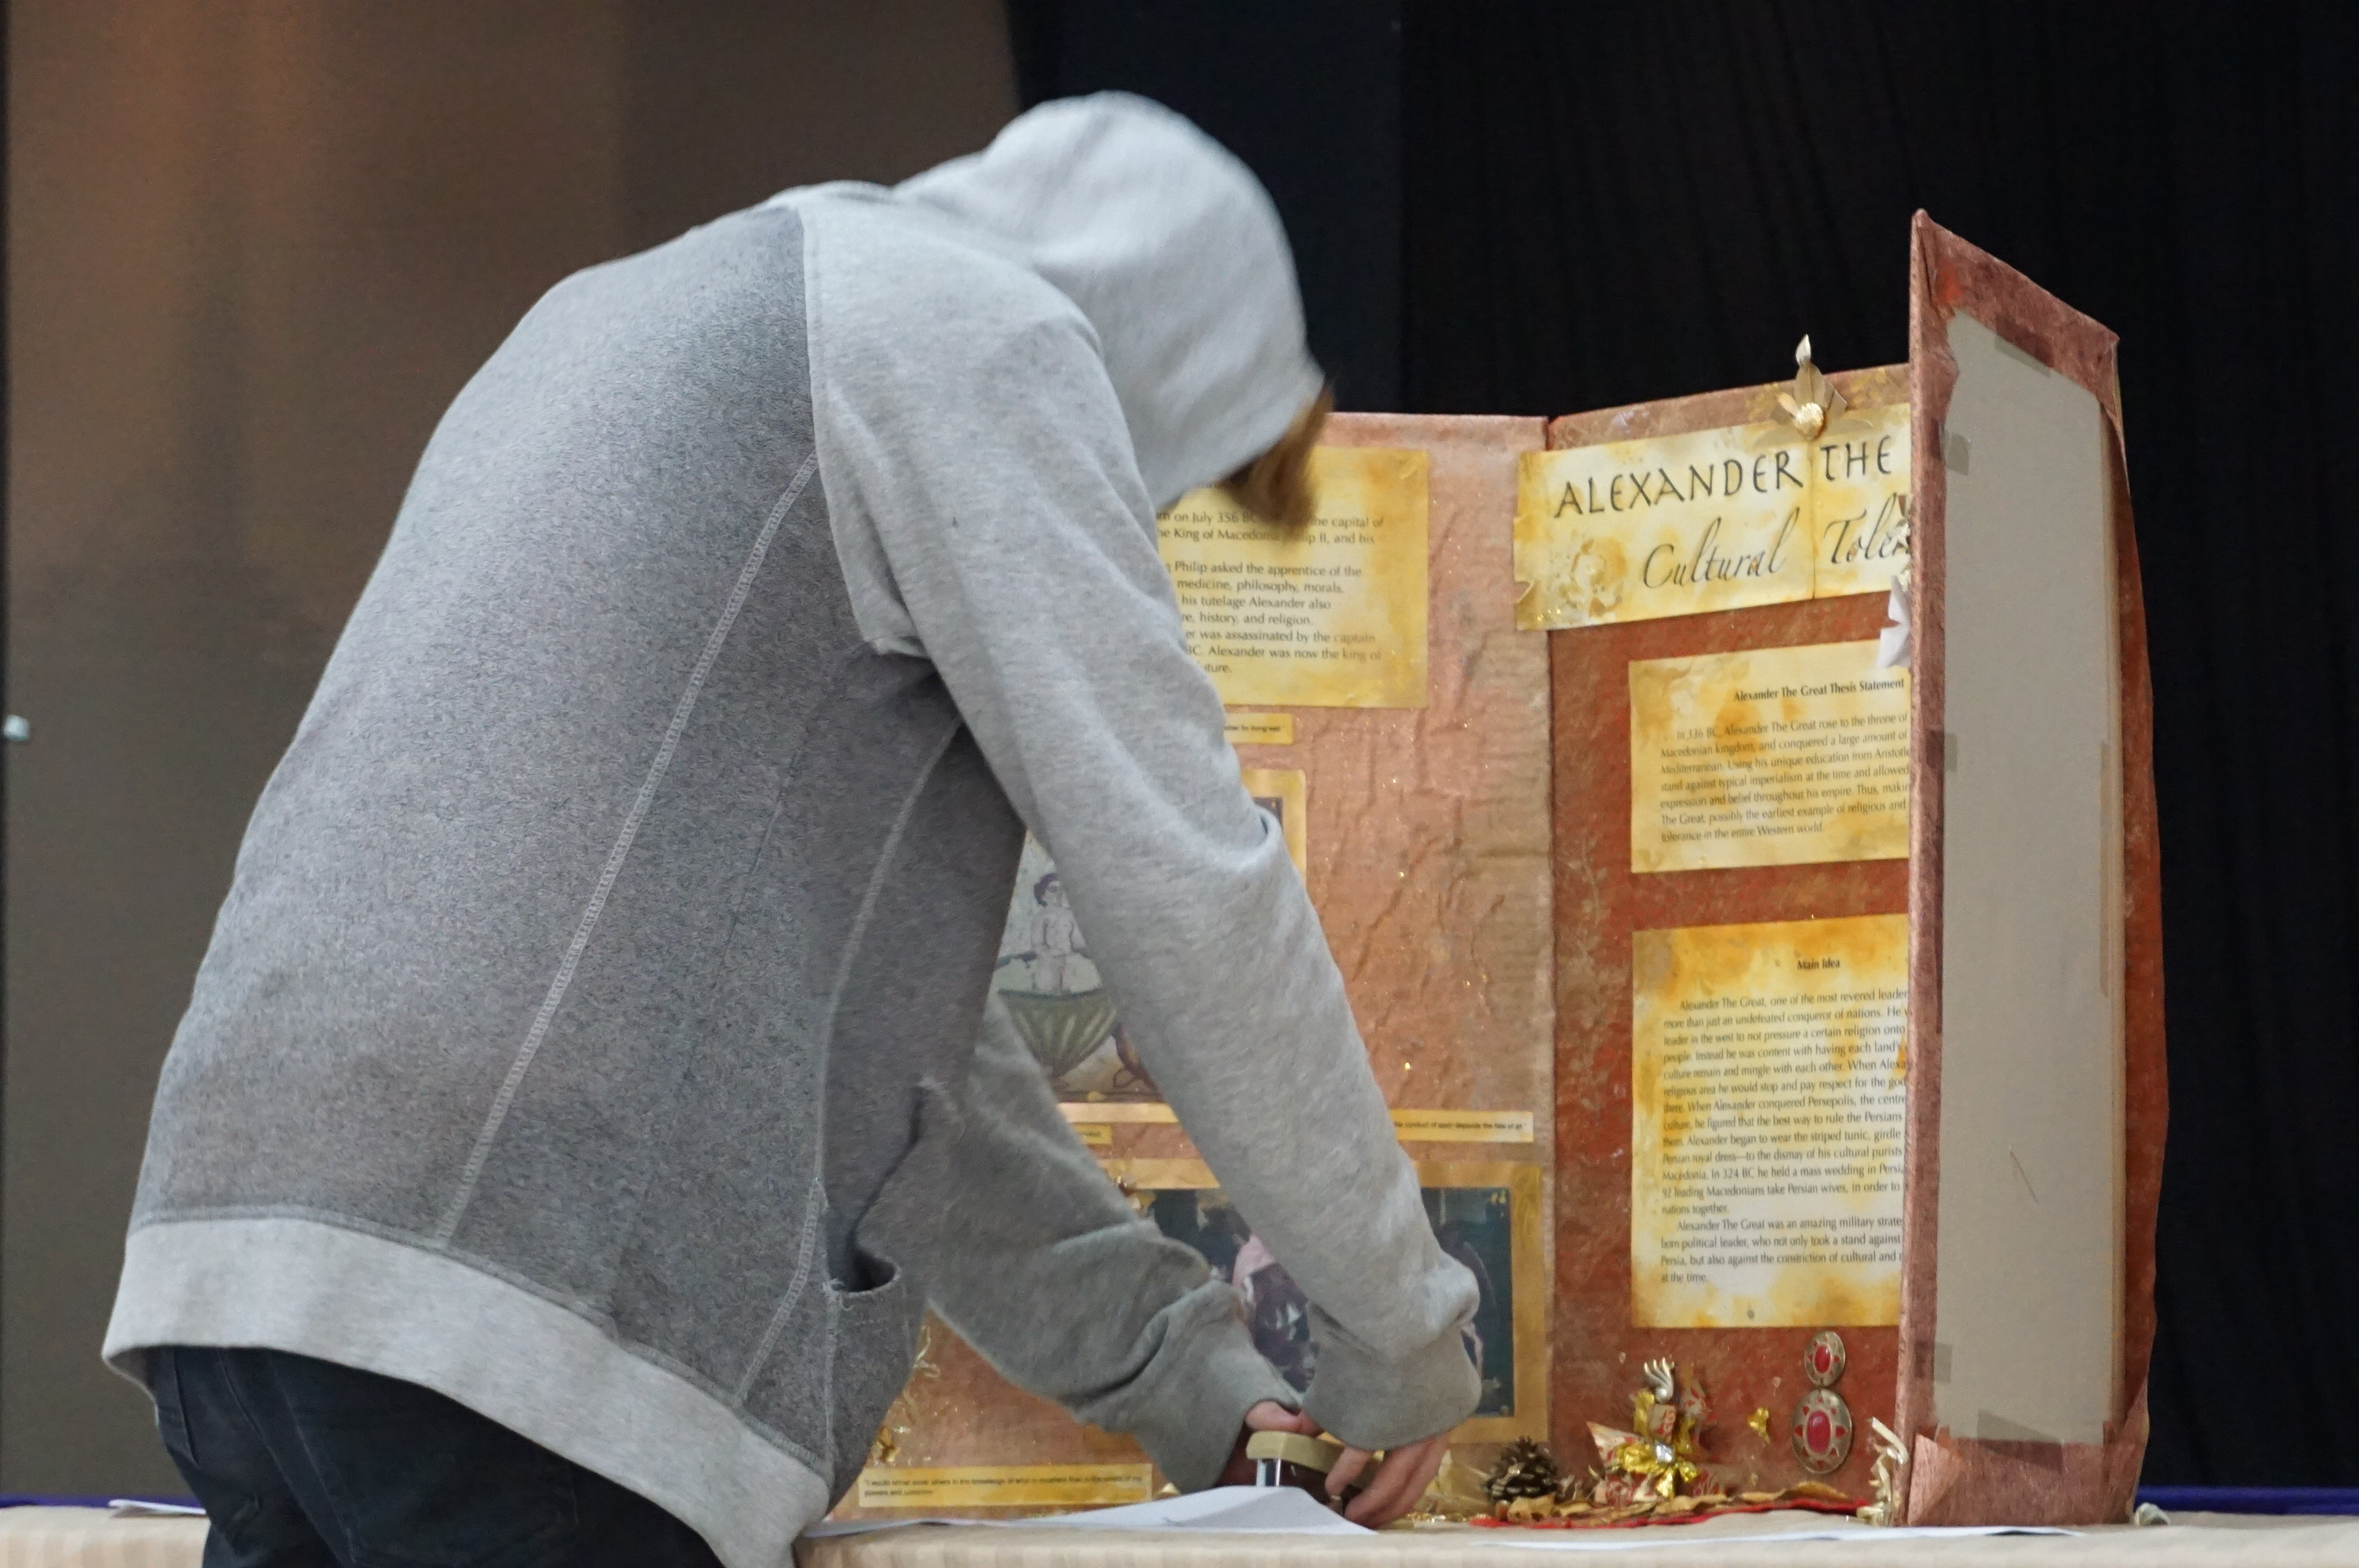
\includegraphics[width=\textwidth]{chapter4_B1_p3.jpg}}


\subsubsection{Conclusions}
\prompt{Comment on the degree to which this criterion is being addressed.}

\begin{findings}
The findings suggest that CMIS addresses the What Students Learn criterion to a high degree. Though CMIS has made a great deal of progress since the last self study visit and the mid term report, much more work needs to be done. In addition to the specific places of growth found “so what” section of each indicator, below is an further analysis of the What Students Learn criterion findings:

\minor{Maintain and Monitor}

\begin{itemize}
\item Adopted curriculum that is aligned to adopted standards. Maintain curriculum in cycle to be reviewed, vetted, and updated
\item Adoption review cycle, resource request form, resource renewal form
\item Course offering to ensure rigor, relevance, and coherence
\item CMIS adopted standards 
\item CMIS Adoption Protocol. Newly adopted curriculum vetted for rigor, alignment, and engagement. Cannot be said for older curriculum. 
\item Structures to ensure alignment of standards to actual concepts through vetted curriculum, adjustments to UbDs, instructional rounds, formal evaluations, and blueprints. 
\item Special needs students using the protocols in place 
\item Assessment alignment to standards and rigor of standards
\item Programs, curriculum, and planning that requires authentic integrations among disciplines (NHD, PARCC, UdD, disciplinary literacy, literacy blocks, new curriculum etc.)
\item Adoption review cycle 
\item Curriculum design/adoption cycle. Continue to emphasize looking at student work as data to make curricular and instructional decisions 
\end{itemize}

\minor{Continue to Improve}

\begin{itemize}
\item Student accessibility based on research-based practices
\item Process that invites all stakeholders to assess curriculum (i.e. parents and students)
\item Programs that strengthen ties with other educational institutions and continue to look for new opportunities 
\item Frequency of looking at student work protocols
\item Vetting curriculum for emphasis on global concepts, perspectives, issues
\end{itemize}

\minor{Investigate Better Practice}

\begin{itemize}
\item Workflow platform to improve resource request and renewal processes 
\end{itemize}

\minor{Proposals for Improvement}

\begin{itemize}
\item Course offering decisions based upon updated demographic of students 
\item Professional development opportunities based on deliberative practice for teachers 
\item Follow up studies in college and career preparedness
\end{itemize}

\end{findings}

%%%%%%%%%%%%%%%%%%%%%%%%%%%%%%% How students learn %%%%%%%%%%%%%%%%%%%%%%%%%%%%%%%%%

\subsection{B2 How Students Learn Criterion}
\subsubsection{Research-based Knowledge}

\indicator{The administrators and teachers use a variety of approaches to remain current in research-based professional knowledge and apply the knowledge to improve teaching and learning. All students regardless of background and ability are actively involved in the learning that is based on the schoolwide learner outcomes and academic standards.}

\prompt{ Provide a range of examples that demonstrate teachers are current in the instructional content taught and research-based instructional methodology.}

\begin{findings}
CMIS Leadership and Teaching Staff use a variety of approaches to remain current in research-based professional knowledge.

\minor{Standards, UbD, and Datawise}

Three broad themes are the cornerstone of professional development to keep CMIS Leadership and Teaching Staff current in research-based professional knowledge: \href{https://drive.google.com/drive/folders/0B71_pYxcTLo-NGJ4N0RQWXRTNE0?usp=sharing}{standards}, \href{https://docs.google.com/a/cmis.ac.th/document/d/1kL1VjwfuMMa7NaWmwUrEah1BM-jJRmLAd4VJzR3HoPs/edit?usp=sharing}{Understanding by Design}, and \href{https://docs.google.com/a/cmis.ac.th/presentation/d/1omzyjfwf5fazGCSuvw7dDQn4eqhpOIaldeLXY7-6PYQ/edit?usp=sharing}{Datawise}. As these three topics are the umbrella of professional development, underneath this umbrella contained numerous micro topics in which the staff focused on. See \href{https://docs.google.com/a/cmis.ac.th/document/d/1Xi1oHSwcvMUAaFtHW9SU3m1QJpIRRrmdphVHokoJsI8/edit?usp=sharing}{Table 3} for an outline of these topics, note that complete fluency in and fidelity to these topics is ongoing. Each major topic encompasses both content and methodology. 

Though each major topic is interrelated with each other, there were additional research-based concepts that were embedded in the professional development. These include \href{https://drive.google.com/drive/folders/0ByVFfrm0zfolQ3FRNWNSVmpCUUk?usp=sharing}{instructional rounds}, \href{https://drive.google.com/drive/folders/0ByVFfrm0zfolaFNZMDVFZnFLazA?usp=sharing}{formative}/\href{https://drive.google.com/drive/folders/0ByVFfrm0zfolczUtZFkzUldXQnM?usp=sharing}{summative} best practices, \href{https://drive.google.com/drive/folders/0ByVFfrm0zfolWW5aWGZOUjVJTm8?usp=sharing}{looking at student work}, and \href{https://drive.google.com/drive/folders/0ByVFfrm0zfolWFNfWGRuWDlxUDQ?usp=sharing}{SMART goals}. Each of these topics complemented the work of the major goals. 

{\centering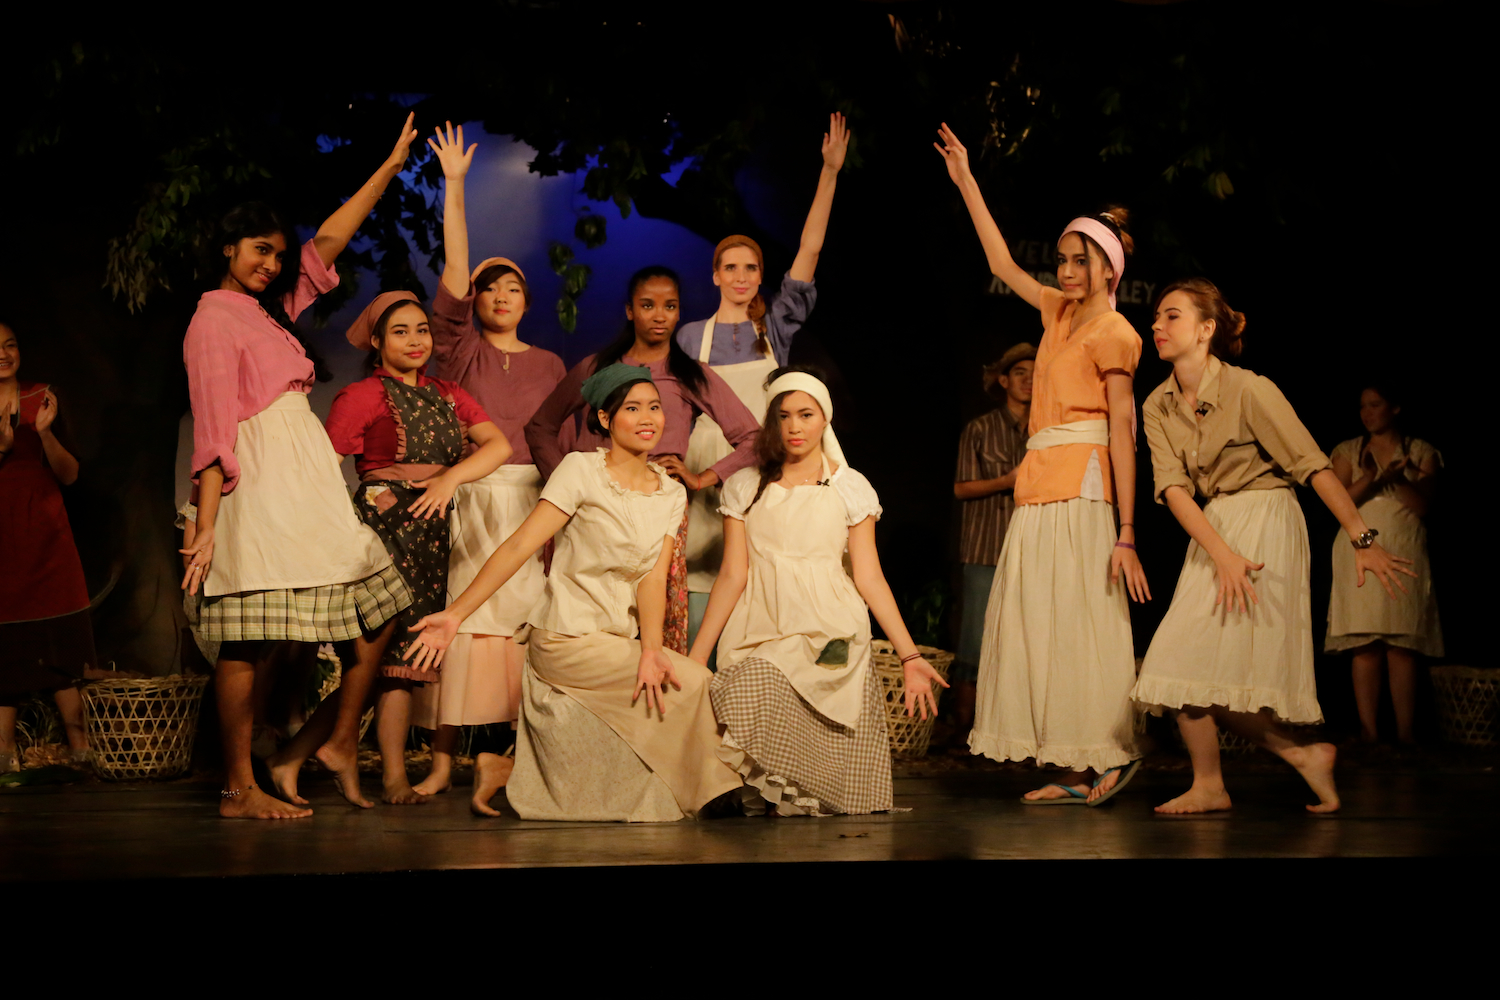
\includegraphics[width=\textwidth]{4_2_1_hl_a.jpg}}

CMIS Staff are provided with a variety of approaches to access the major/micro goals. Early release, scheduled professional development meetings are held once a month. During this time, whole/small, and department, mixed, or interdisciplinary groups are organized for collaboration. Separate department and division meetings are also scheduled once a month where a percentage of the time is devoted to current, research-based topics. Other organizational structures are used to access research. See Professional Collaboration indicator in What Students Learn section for a detailed list of collaboration models at CMIS and the CMIS Curriculum/Instruction Action Plan for a list of professional development trainings since 2014. 
 
\minor{Research-Based Resources}

Numerous vetted and juried journals and organizations are used for the CMIS Leadership and Staff to remain current on both research-based content and methodology. See \href{https://docs.google.com/a/cmis.ac.th/document/d/1xIQ3-59L8c4iTP9yB2HinT_vkMM5EzrZw17NmjZSzOE/edit?usp=sharing}{Figure 4} for a breakdown of these organizations. 

CMIS Staff that have an Advanced Placement assignment have remained current, not only of the unique elements of AP class methodology and content, but of the regular updates in specific AP courses and exams. 

\minor{Outside Professional Development}

For a number of years, CMIS has organized or has been a participating member of the yearly Chiang Mai Circle of International School Conference (CMCISC). The conference  theme changes each year and provides CMIS Staff an opportunity to work in collaborative teams, network with peers (in job share-alike discussions), and take brief workshops mostly lead by teachers on topics that align with the yearly theme. Along with 100\% staff attendance at the CMCISC conference, the past two Conferences saw five CMIS staff members present on topics such as text complexity, formative assessment, and classroom management. See 2015 CMCIS Conference Presentation \href{https://docs.google.com/document/d/1dFBXhPjlnErh-Sd2tAF0o2A8gXC37B4h2dEWAnCKhOY/edit?usp=sharing}{Catalog} and the 2016 CMCIS Conference Presentation \href{https://docs.google.com/document/d/1mT0c3_-WV7xRc-BbgpTU6cae63VlS3sN9sr-8q1Lid0/edit?usp=sharing}{Catalog} for more information. 

CMIS has had the opportunity for our Head of Department for Science, Graeme Ritchie, to secure an EARCOS Action Research grant. His research, entitled \href{https://drive.google.com/file/d/0B7TDqZfXoqRrLThkSjg0MFRvWkk/view?usp=sharing}{Inside the Engine Room of Learning}, studied the frequency, quality, and categories of student-to-student interaction in the middle school science classroom.  

\minor{So what...}

Using researched based information to inform our decisions is a strong area for CMIS. The focus on using research-based strategies and process  involves jargon and processes that the CMIS Leadership sometimes assumes the staff understand and/or have used in the past. CMIS Leadership should ensure that steps are embedded in the professional development and training to access prior knowledge and experience of the participants. This would enable them to provide the PD at a level that would be most beneficial to the teachers, and differentiate it to best meet their individual needs and abilities.
\end{findings}

{\centering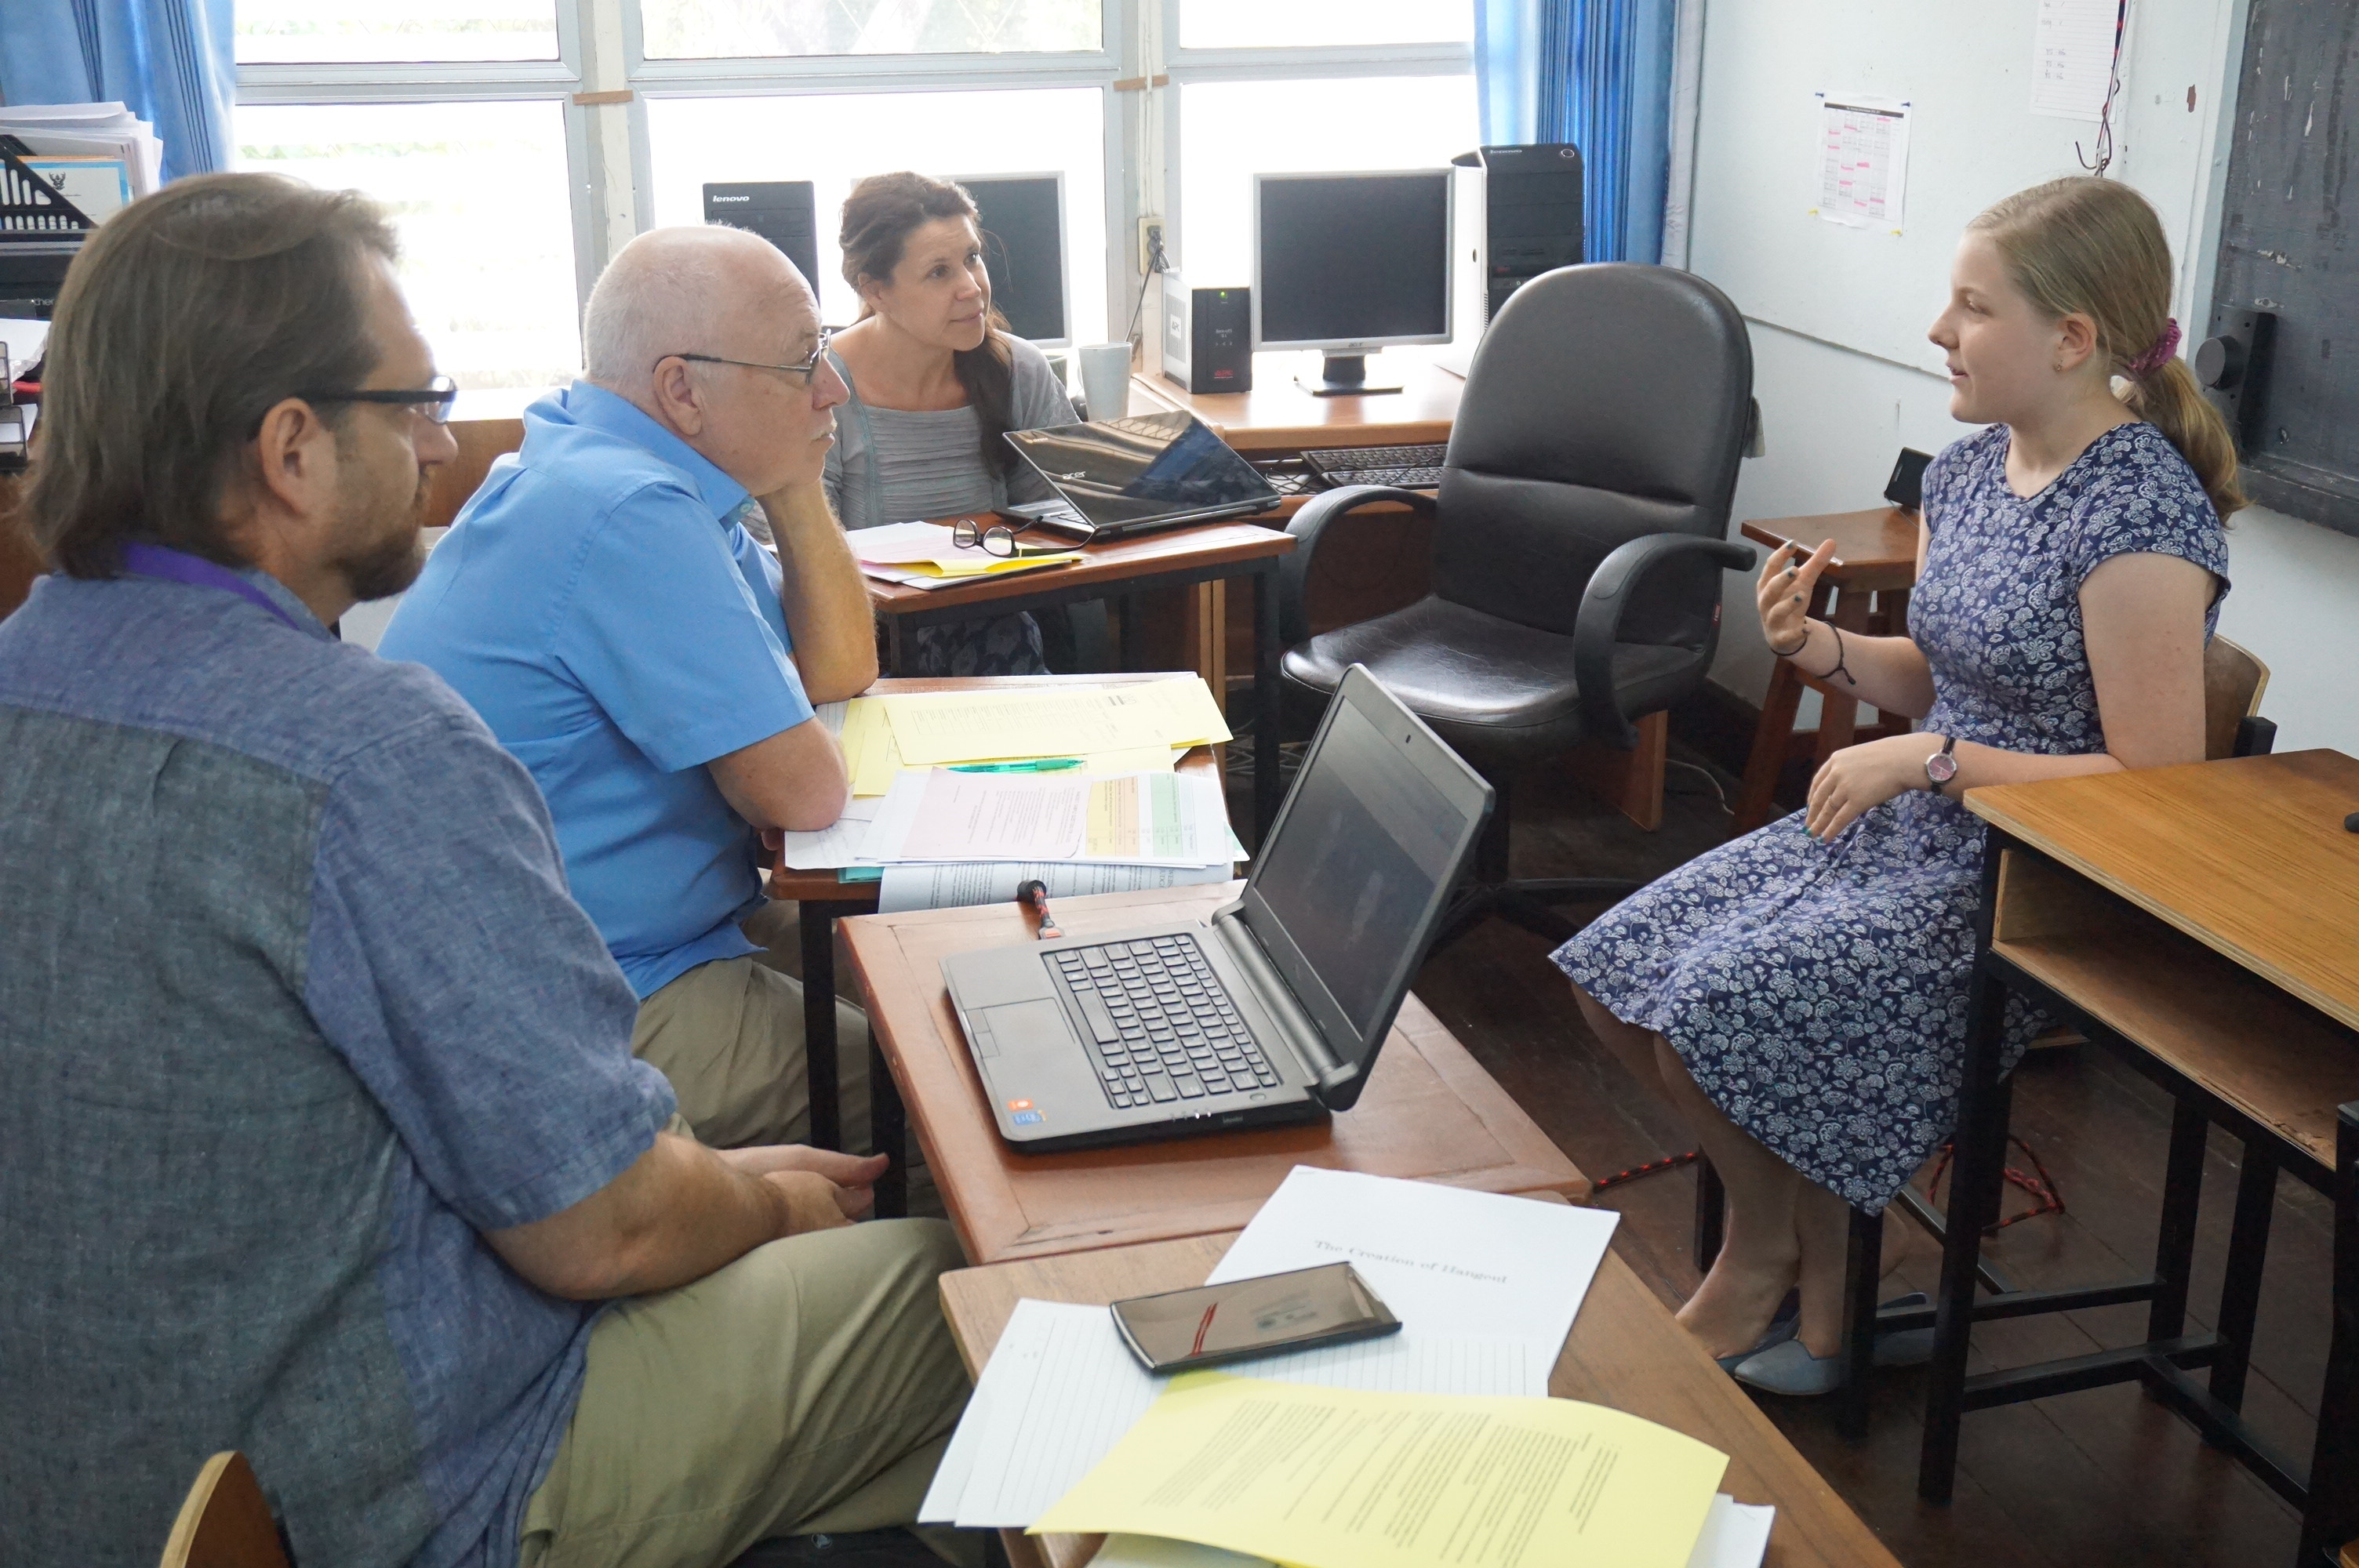
\includegraphics[width=\textwidth]{chapter4_B2_p1.JPG}}

\subsubsection{Planning Processes}

\indicator{The planning processes, including the use of formative assessment results, focus on the engagement of all student activity at a high level of learning consistent with the academic standards and schoolwide learner outcomes, i.e., global competencies.}

\prompt{Comment on the effectiveness of the planning processes, including the use of formative assessment results, to engage all students actively at a high level of learning consistent with the academic standards and schoolwide learner outcomes.}

\begin{findings}
The use of data by CMIS Leadership and Teaching Staff has played a central role in the planning processes to ensure rigor and alignment to the standards. 

\minor{Datawise a Data Analysis Process}

CMIS Teaching Staff and content departments use data to make planning decisions. CMIS Teaching Staff and departments use department meetings, divisional meetings, and early release meetings to make decisions about the effectiveness of instructional planning. In the past, decisions made in these meetings have focused on the purchase of resources, assessment creation/results, student achievement and behavior. 

As described in other indicators, CMIS Leadership and Teaching Staff have used the Harvard Graduate School of Education’s \href{https://docs.google.com/a/cmis.ac.th/presentation/d/1omzyjfwf5fazGCSuvw7dDQn4eqhpOIaldeLXY7-6PYQ/edit?usp=sharing}{Datawise} process to analyze student data to identify a learner centered problem (LDC) and a problem of practice (POP). This LDC and POP are used to help the staff select a research-based instructional strategy that is aligned to the standards and is embedded in our instructional planning  throughout the year. The goal of Datawise is to use a research-based structure to make data analysis and data decisions a consistent, continual practice at CMIS; to make a school culture of using using data, rather than a singular event to fulfill the WASC self-study requirements. 

\minor{Formative Assessment Focus}

Formative assessment has been a regular focus for the past two years. CMIS Leadership and Teaching Staff have spent time clarifying and defining what formative assessment is and is not. Though some CMIS teachers use formative assessment regularly to evaluate student understanding of a concept,  using formative results to differentiate students in small group based on skill deficiency or using the results to adjust the learning strategies is still a work-in-progress. Though a continuing focus, some CMIS teaching staff have skillfully used interactive formative tools such as Quizlet, Kahoot, and Google Forms to effectively collect student data. See \href{https://docs.google.com/a/cmis.ac.th/presentation/d/1S1x1yEj7KDD6jM7u1RdTZJEt10_0r6mcJ-LmRb6iPWs/edit?usp=sharing}{Formative Assessment and Productive Failure} workshop and the \href{https://drive.google.com/drive/folders/0ByVFfrm0zfolaFNZMDVFZnFLazA?usp=sharing}{Formative Assessment Resources} folder for more information. 

CMIS has made strides in ensuring that formative assessment is central part of any discussion about planning and instruction; for example, CMIS has made modifications to the UbD template  to include a stand alone, formative assessment section and HS has created a non-graded category on the Powerschool online student grade platform to track formative assessments. When asked to describe how they formatively assess their students, CMIS teachers will describe how they:

``Practiced skills in a review game to give the students an opportunity to discuss areas that they did  not fully understand and to focus on reviewing those skills.''

``Use exit tickets based on the goals of the week [which] help to highlight who understood the key ideas we explored and who is still processing the content.''

``Asked the students to write down sentences using their spelling vocabulary and could see which words they understood and which words they need to understand more.''

``Did the mid-year datawise assessment that showed that while progress has been made, not all of the students in the class were able to effectively design an experiment, or did not yet understand some of the critical components of experimental design and need additional review/practice.''

Based upon 2015 teacher perception data, 65\% of the CMIS Teacher respondents felt confident or very confident using formative assessment. See \href{https://docs.google.com/a/cmis.ac.th/forms/d/1-00JLey-jyLuizymm8z8JGJ6iLp4l-ccsTgHJ_Ckcj8/viewanalytics}{Professional Development Reflection} for more information. 

{\centering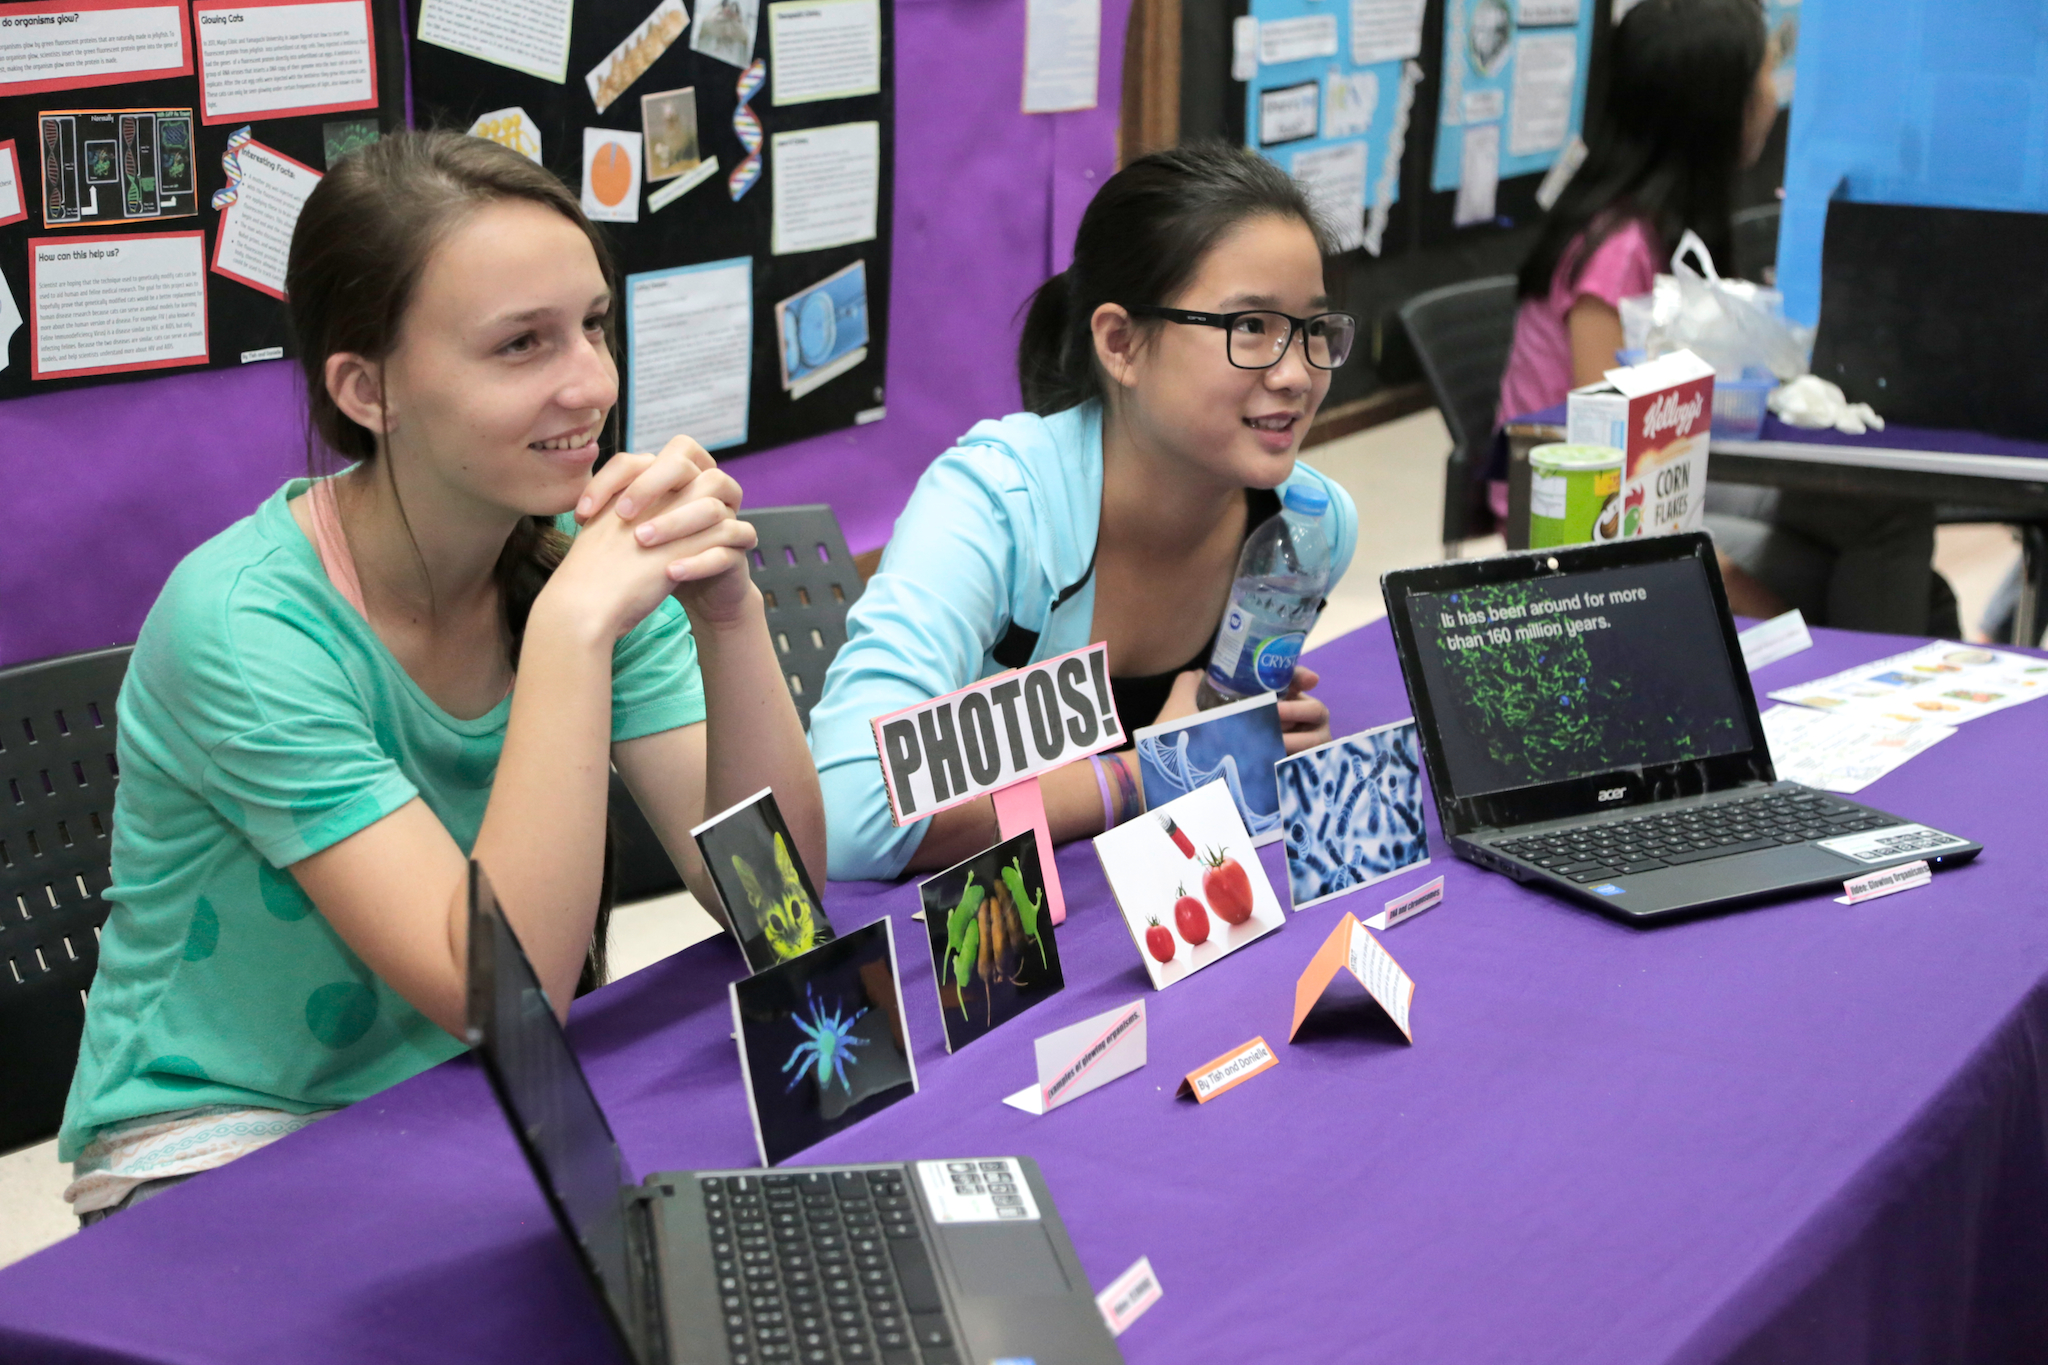
\includegraphics[width=\textwidth]{4_2_1_hl_b.jpg}}

For more insight on formative assessment at CMIS, see the section entitled: Acceptable Student Achievement, Modifications/Decisions Based on Assessment Data, and Appropriate Assessment Strategies. See \href{https://docs.google.com/a/cmis.ac.th/document/d/1yPhINDe21ApcJp3psbSCgmS9PHEBbxrCflrR2Adnwho/edit?usp=sharing}{Formative Assessment Snapshots} for anecdotes on how CMIS Teachers use formative assessment. 

\minor{Diagnostic Assessment}

All KG-5 use two diagnostic assessments to ensure quality planning: \href{https://drive.google.com/drive/folders/0ByVFfrm0zfolV29lcmM1WXVQOXc?usp=sharing}{DRA} (Developmental Reading Assessment) and the \href{https://drive.google.com/drive/folders/0ByVFfrm0zfolLU9Vb0ZBeF9uZjQ?usp=sharing}{CMIS Common Writing Pre assessment} (during the 2015-2016 school year). Both assessments are used by some of the CMIS Teaching Staff to inform divisional and grade level planning. For example, the common writing pre assessment was used by the English and social studies department to construct a common argumentative rubric using the pre assessments as anchor papers. This rubric was also used in planning of the UbD units in both departments. 

\minor{So what...}

CMIS has made significant strides in the understanding of formative assessment and a handful of teachers use the formative data skillfully and strategically. Data also indicates that formative assessment is used more frequently than in previous years. CMIS would benefit from time and resources used to train some teachers on transitioning from good formative assessment to great formative assessment. Good formative assessment is giving it and using the data to inform your (i.e. the teacher’s) future instruction. Great formative assessment is involving the students in the data results to make achievement for all students in all courses/grade levels a reality. Additionally, planning processes should be designed with an emphasis on global competencies and the schoolwide learner outcomes more explicitly. 
\end{findings}

\subsubsection{Professional Collaboration}

\indicator{ Administrators and teachers use various collaborative strategies to examine curricular design and student work to improve learning and teaching, including demonstrating critical thinking, problem solving, knowledge, and application. This would include examples of the selection of the instructional approaches based on the learning purpose(s) desired.}

\prompt{ Comment on how administrators and teachers use various collaborative strategies to examine curricular design and student work to improve learning and teaching, including demonstrating critical thinking, problem solving, knowledge, and application. Include examples of the selection of the instructional approaches based on the learning purpose(s) desired.}

\begin{findings}
CMIS Teaching Staff and Leadership use a variety of collaborative strategies to examine curricular design and student work. 

CMIS Leadership strongly believe in the use of protocols during staff collaboration to promote participation, build trust, and ensure equality (McDonald, 2007)

Prior to using any data, general meeting norms are reviewed as well as the three special data norms: assume positive intent, take an inquiry stance, and ground statements in evidence (City, 2007). When looking at student work and curriculum, the use of protocols and norms is important for a variety of reasons. Not only does it ground and focus our work to the meeting objectives, it also provides common expectations and routines which all participants follow. Most importantly, using norms and protocols maximizes participation and ensures all voices are heard. 

{\centering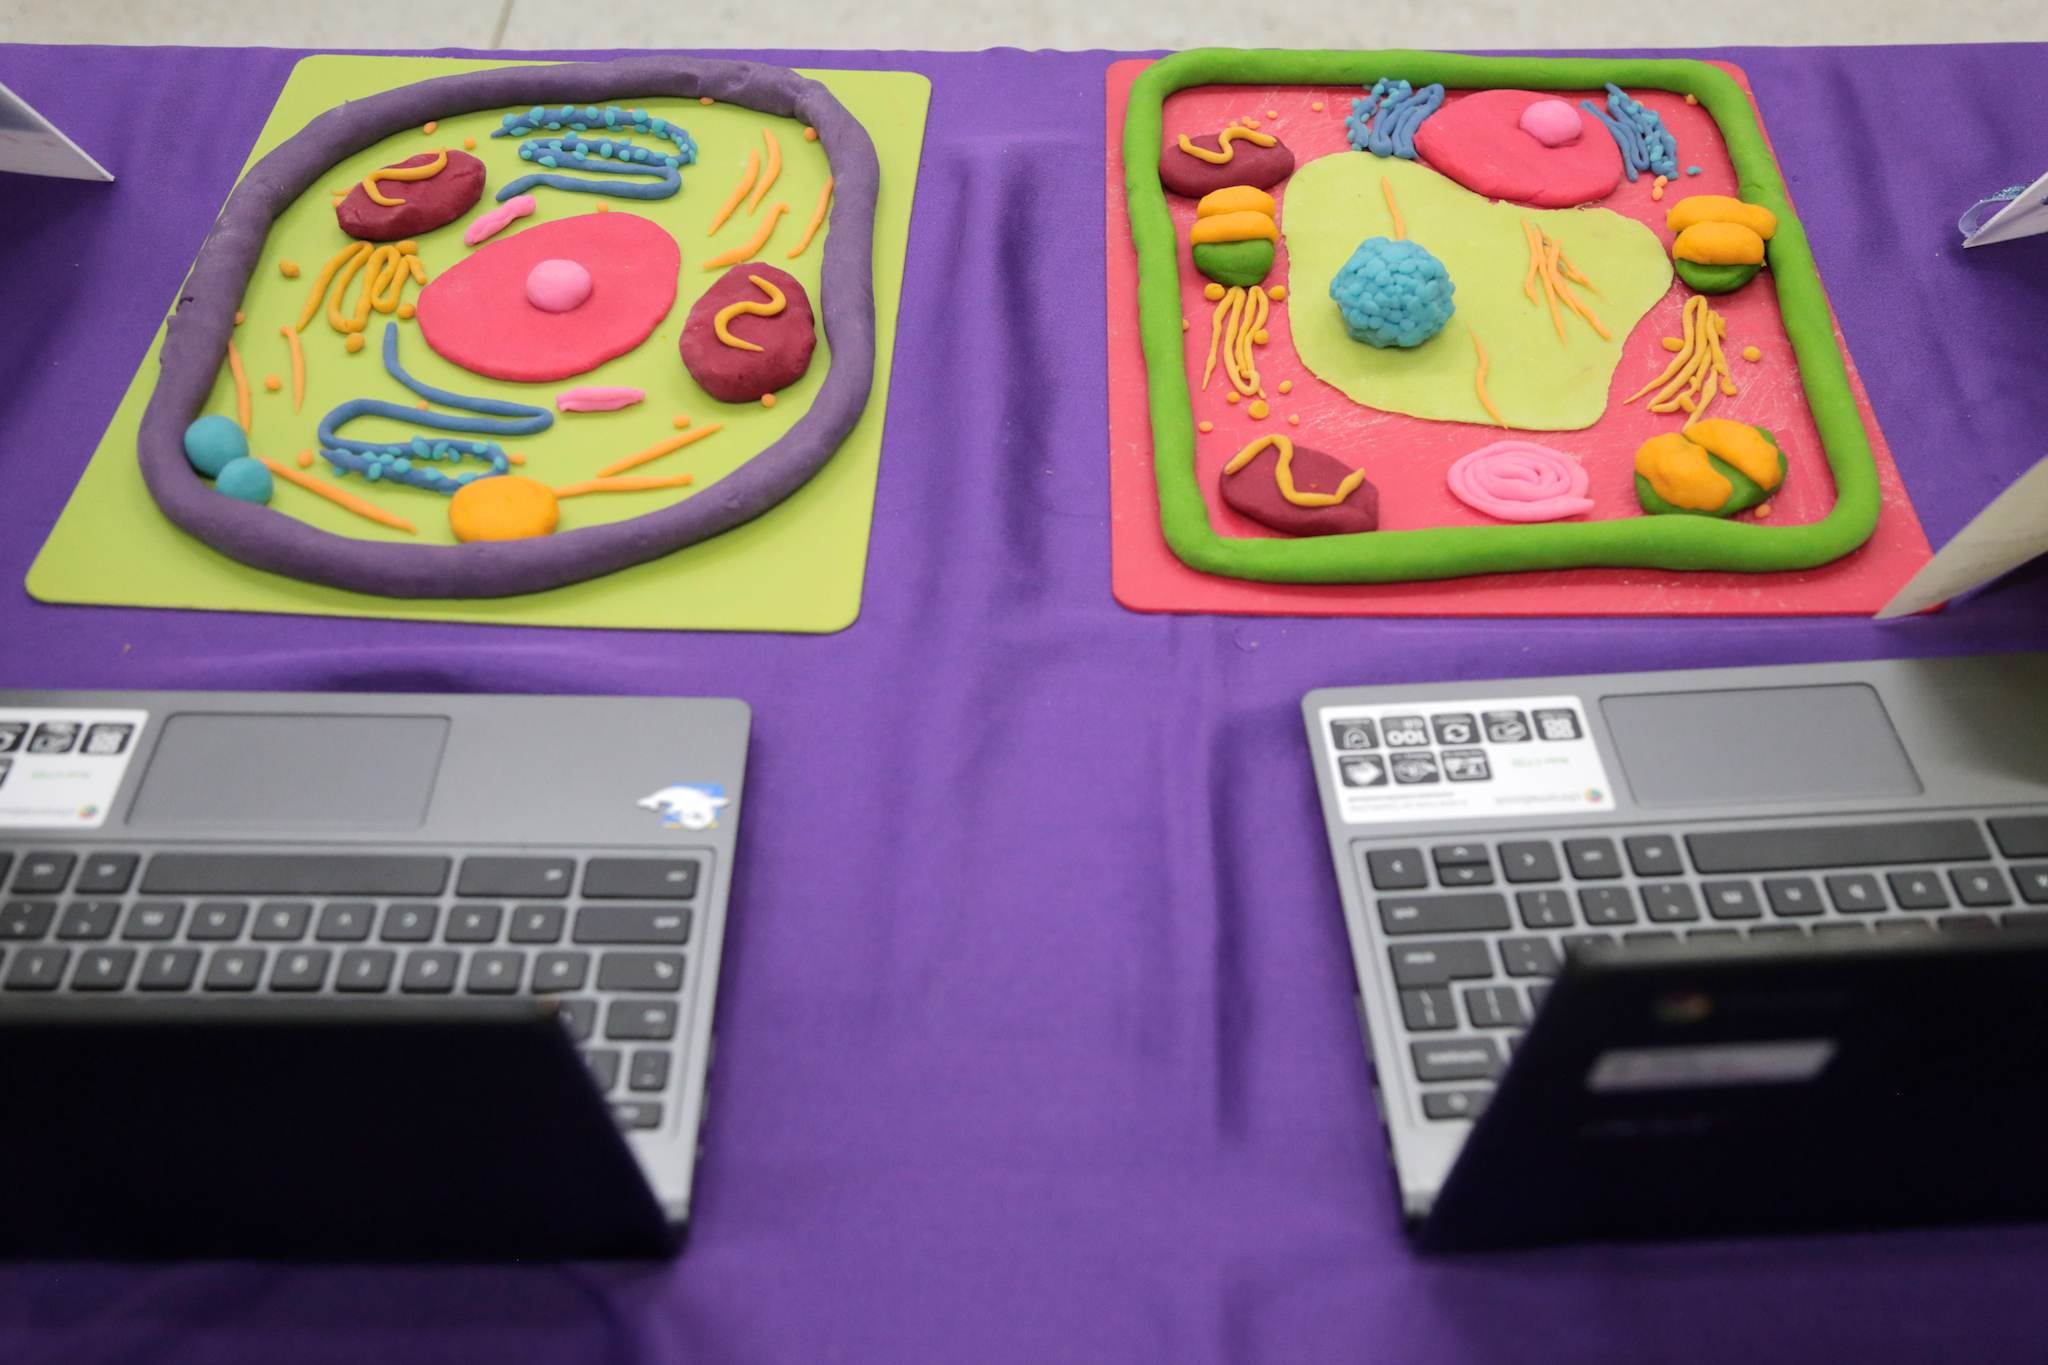
\includegraphics[width=\textwidth]{4_2_1_hl_c.jpg}}

Beginning in the Spring of 2016, CMIS began using a structured and research-based protocol for looking at student work that would provide more specific information to the teachers and more school-wide data (e.g. alignment to the standards, curriculum gaps/redundancies, problems solving, SLOs). CMIS Leadership asked the Teaching Staff to use the \href{https://docs.google.com/a/cmis.ac.th/document/d/1aobA3IksQDoGJ-JKci0YDfFDCgT2ugHM7r_T4i_CL7o/edit?usp=sharing}{Longfellow Slice}, the CMIS Leadership added a handful of focus question to align it more with our SLOs, so it became the Modified Longfellow Slice. During early release meetings, department groups were organized to look at students work with this modified protocol. Participant feedback suggests that more modifications are required to continue to increase teacher relevancy. 

Other protocols have also been utilized to ensure maximum engagement and that “all voices are heard”. These include ATLAS Data Protocol, Warm/Cool Feedback, Notices and Wonderings, and Collaborative Assessment Conference. 

Other strategies used to examine curricular design and student work to improve learning and teaching include:
\begin{itemize}
\item Inter-rater reliability-used on numerous occasions to ensure reliability in grading (e.g. common argumentative rubric meetings) and in unit construction (e.g. UbD Interrater meeting). See UbD Interrater Practice \href{https://docs.google.com/presentation/d/18f8rB_VHa8vQhp-cbmgXFCCJEZ0QB3QkEIp2BiChwyM/edit#slide=id.gd6a9d401a_3_0}{Agenda/Presentation} 
\item Peer review-used consistently for the CMIS Summative Assessment/Final Exam feedback meetings organized once a semester. Protocols become more structured as time progresses. See Summative Assessment Peer Review: \href{https://drive.google.com/a/cmis.ac.th/folderview?id=0ByVFfrm0zfolTHY0dmtURG5pcGs&usp=sharing}{Fall 2014}, \href{https://drive.google.com/a/cmis.ac.th/folderview?id=0ByVFfrm0zfolaWQzeWxCTlVyUFU&usp=sharing}{Spring 2015}, \href{https://drive.google.com/a/cmis.ac.th/folderview?id=0ByVFfrm0zfolRjQzTDhmT0dyYzg&usp=sharing}{Fall 2015}, \href{https://drive.google.com/a/cmis.ac.th/folderview?id=0ByVFfrm0zfolT29vQXpQeXp3VlU&usp=sharing}{Spring 2016} 
\item \href{https://docs.google.com/a/cmis.ac.th/presentation/d/1GDBfSgHVsW5KKXvlBzm-JipLzBO_tWI0R1TlEOwIZ88/edit?usp=sharing}{Depth of Knowledge (DOK)}- Focuses on complexity of content standards, assessment items, or instructional tasks The outcome (product) is the focus of the depth of understanding. Training began in Fall, 2016. 
\item Teach for Success (T4S)- observation protocol; WestEd' s Teach for Success is a focused, collaborative, research-based framework and process that improves K-12 student achievement by improving classroom instruction. The T4S provides a common vocabulary for discussing good teaching. See T4S \href{https://docs.google.com/a/cmis.ac.th/spreadsheets/d/1ACz3l3DPUgIqRhmZ1LWk9RwVBjo0iLsbJAupJoic5Dg/edit?usp=sharing}{Classroom Observation Protocol}.
\item Resource Vetting Instruments- allow teachers and leaders to to focus on understanding the adopted standards and align resources to the rigor found with the standards. 
\end{itemize}
See indicators entitled Collaborative Work for more information on collaborative structures and Challenging and Varied Instructional Strategies for Teacher for Success data on the frequency of use observed.   

\minor{So what...}

CMIS  uses a variety of collaborative strategies and tools to look at student work, evaluate resources, unpack standards, and analyze rigor. CMIS should continue to maintain and monitor these structures for consistency and frequency. 
\end{findings}

\subsubsection{Professional Development}

\indicator{The school uses ongoing professional development to enhance the curriculum and improve learning and teaching. This includes learning through worldwide partnerships with other teachers and schools.}

\prompt{Comment on how the school uses ongoing professional development to enhance the curriculum and improve learning and teaching.}

\begin{findings}
CMIS Leadership and Teaching Staff are continuing to find the right balance of in-house vs outside and school-wide vs  individualized professional development opportunities. CMIS professional development philosophy revolves around two questions:

\begin{enumerate}
\item Is the professional development backed by research, including does it involve enough time to have an effect on student learning?
\item Is the professional development consistent with our standards and current initiatives? 
\end{enumerate}

{\centering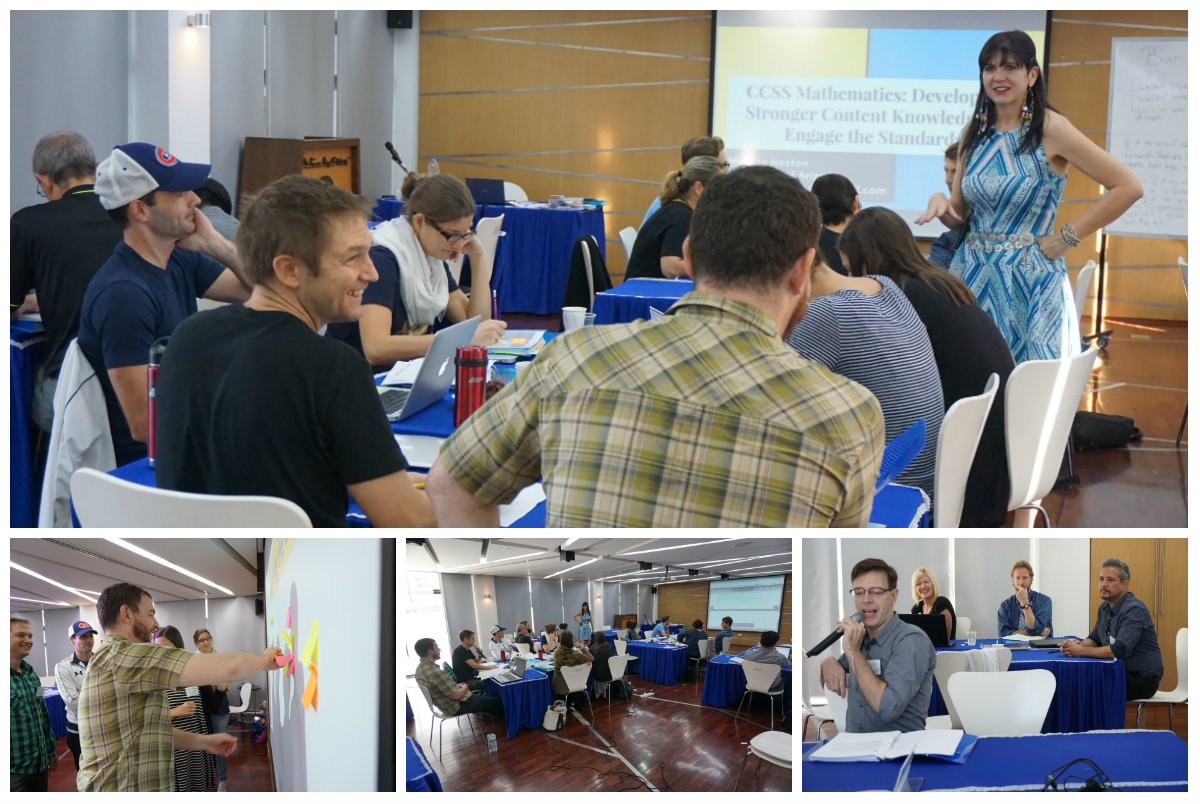
\includegraphics[width=\textwidth]{chapter4_B2_p2.jpg}}

\minor{Backed by Research}

For school wide opportunities, all professional development planning has been aligned to best practices and the existing adult learning research. CMIS Leadership adheres to current research which states that teachers who receive well-designed professional development, for an average of 40 hours (CMIS literacy/assessment focus was at approximately 50 hours in 2014-2015) spread over six to 12 months, can increase student achievement by as much as 21 percentile points (Yoon, Duncan, Lee, Scarloss, and Shapley, 2007). CMIS Leadership would like to encourage moving away from the one-shot, "drive-by," or fragmented, "spray-and-pray" workshops lasting 14 hours or less which show no statistically significant effect on student learning (Darling-Hammond, Wei, Andree, Richardson, \& Orphanos, 2009). Above all, CMIS Leadership would like to continue to move towards implementing effective professional development programs are job-embedded and provide teachers with five critical elements (Darling-Hammond et al., 2009):

\begin{description}
\item [Collaborative learning] Teachers have opportunities to learn in a supportive community that are normally organized by content department or grade level. CMIS would like begin scheduling more professional development opportunities for K-12, that are organized in small-flexible groups, across grade levels and contents. Currently, depending on the focus of the training, groups are organized homogeneously by content or grade level band, or heterogeneously, cross disciplinary or grade level (e.g. science curriculum meetings 6-8 and NGSS unpacking)
\item [Links between curriculum, assessment, and professional-learning decisions] Though developing curriculum is still a work in progress, CMIS Leadership has continued to ensure that the analysis of adopted standards and assessment has been discussed hand-in-hand and in the context of the teachers’ content. For example, the CMIS math department understands that research has emphasized the importance of developing math content knowledge, as well as pedagogical techniques for math (Blank, de las Alas, and Smith, 2008; Blank and de las Alas, 2009; Heller, Daehler, Wong, Shinohara, and Miratrix, 2012). Members of the Mathematics department, along with the elementary heads of department, attended Linking Learning and Language mathematics workshop. The objective of this workshop was to deepen their understanding of the challenges and opportunities for sense-making, reasoning, and academic language development of relevant  mathematics concepts in the Common Core mathematics standards (see section entitled Outside Presenters for a description of another, more intense math training at CMIS). Furthermore, the CMIS mathematics department was given some autonomy to work on the unique shifts of the math standards and collaborate on specific pedagogical challenges when the department planned their UbD units. Other examples of linking professional development within the content include: continued unpacking of the NGSS standards during the adoption process, deeper analysis of the literacy standards and shifts during ELA blueprinting, collaborative discussion about content/standards during small group UbD unit study sessions, and developing certain pedagogical moves during C3 social studies training. 
\item [Active learning] CMIS Leadership continues to address how teachers apply new knowledge and receive feedback with ongoing data to reflect how teaching practices influence student learning over time. With the introduction of the Data Wise and Instructional Rounds process in the 2015-2016 and the full implementation in the 2016-2017 school year, CMIS teachers will be able to apply their understanding of the school wide professional development foci, including literacy standards, formative assessment, understanding by design. During Instructional Rounds CMIS Teaching Staff can receive non-evaluative feedback from their peers. Similarly, Data Wise allows the entire CMIS staff to concentrate on collecting and acting on a  specific learner centered problem (LCP) and problem of practice (POP). Part of the process involves specific professional development involving searching for research-based instructional strategies to address the LCP and POP. 
\item [Deeper knowledge of content and how to teach it] CMIS understands that the research does not support training teachers solely in new techniques and behaviors. CMIS Leadership continues to work towards professional development that centers on techniques and behaviors is rooted in disciplinary content. A seemly small, but powerful example of how this is addressed is in the use of our meeting norms, especially the Be Adaptable norm (the others are: Respect Time, Be Present, Be True), at the beginning of every meeting, CMIS teachers are asked to reflect on how each professional development focus relates to their own specific content and/or grade level band. 
\item [Sustained learning, over multiple days and weeks] CMIS Leadership understands that professional-development efforts that engage teachers in 30 to 100 hours of learning over six months to one year have been shown to increase student achievement. CMIS Leadership would like to continue to address sustained professional development. As mentioned previously, the CMIS literacy/assessment focus of the 2014-2015 year engaged teachers in approximately 50 hours of sustained professional development in the Literacy standards. 
\end{description}

Note: the bolded continue(s) in the narrative are meant to emphasize that CMIS Leadership is progressing toward meeting these critical elements. 

\minor{Early Release Wednesday}

Since August 2014, CMIS Leadership has emphasized the early release dates as time to receive professional development. By a large degree, the early release time is CMIS’ biggest investment in professional development. Topic ranging from the close reading process to formative assessment have been presented during this time. Please see CMIS Curriculum/Instruction Action Plan for details on each training. 

{\centering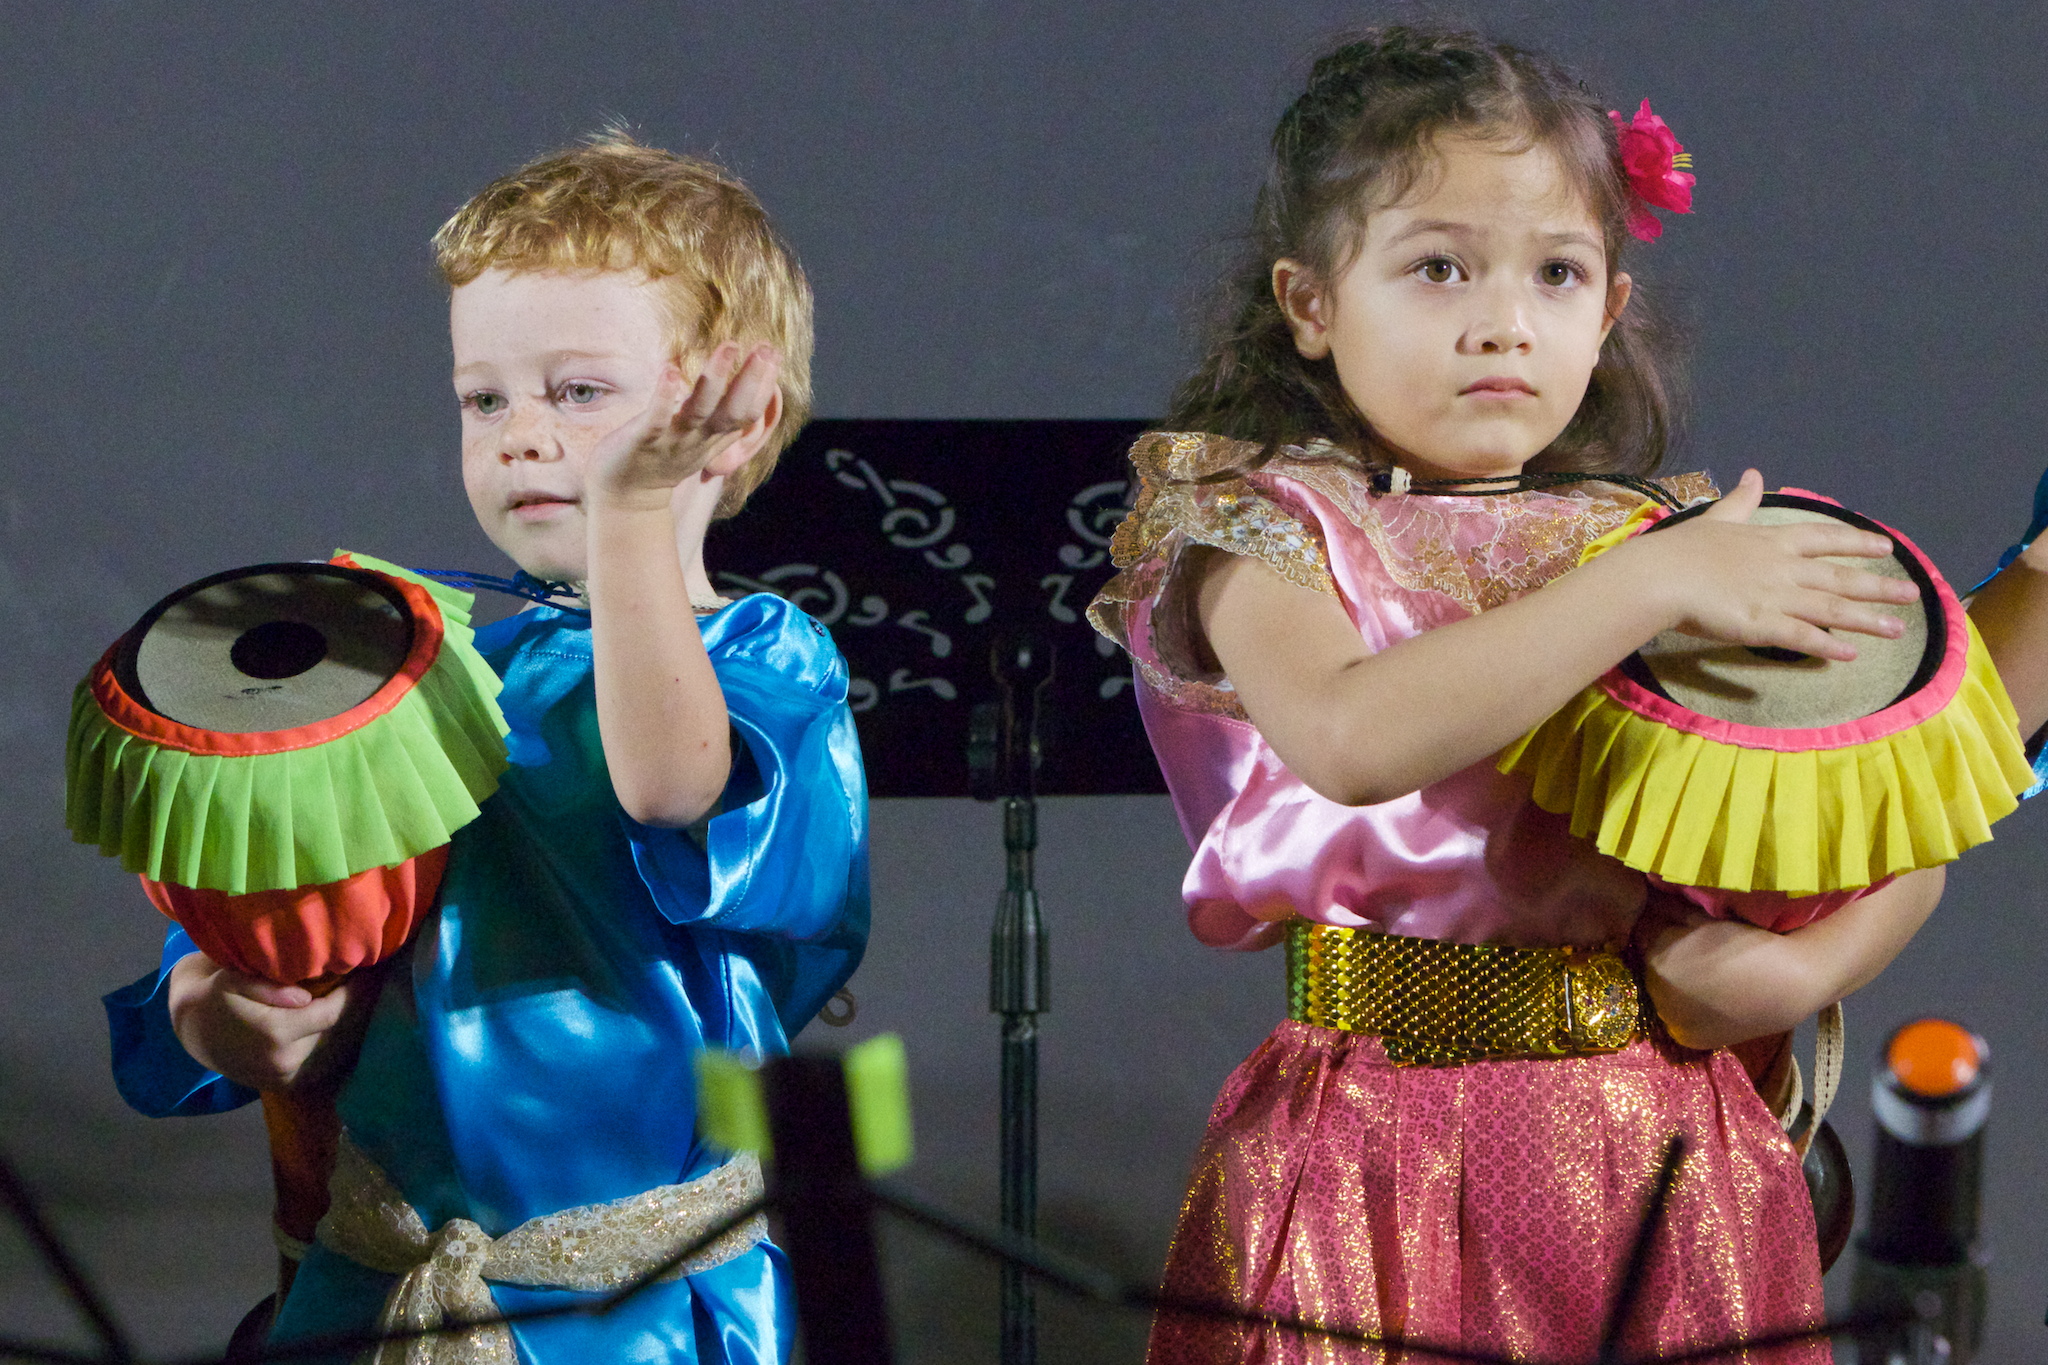
\includegraphics[width=\textwidth]{4_2_1_hl_d.jpg}}

During the 2016-2017 year CMIS Staff will have an opportunity to receive certificates for attending early release professional development training since August 2014. This is an effort to encourage a shift in thinking that professional development can happen on-site. 

\minor{Adoption of Curriculum}

Professional development opportunities are embedded into all adoption meetings. Unpacking standards, discussing essential shifts, alignment of standards to curriculum each involve training and collaboration. See adoption folders for \href{https://drive.google.com/drive/folders/0ByVFfrm0zfoleXEyU3I0cTBXMVk?usp=sharing}{Science} and \href{https://drive.google.com/drive/folders/0ByVFfrm0zfolakRsUVNBaXhWcjQ?usp=sharing}{Math} for more information. 

\minor{Consistency}

The CMIS system for PD funding and application was reviewed in the 2014-2015 school year and a new PD funding system is now in place (see PD Request Forms). The review revealed that on some occasions, professional development was being approved that did not align with our standards or did not address the school-wide instructional or assessment focus, or that it was not content-focused. The revised PD funding process and application was developed to clarify these issues. For example, professional development opportunities have been approved for teachers facilitating a new AP course (AP Computer Science, EARCOS 2015), new to the AP (AP World and US history, on-line, summer, 2016), or away from the course for a number of years, (AP Biology, summer, 2016). PD has also been approved for teachers new to a school-wide initiative (National History Day, Jakarta, 2016). Finally, teachers have gone to training opportunities that center on their content: mathematics, (Linking Language and Learning in Math,  2015), elementary physical education and music best practices (EARCOS, 2016),  In the past two years, CMIS has had five teachers take AP sponsored Summer Institutes for five different classes. The summer of 2017 a staff member will participate in a Daily 5 and Math Daily 3 including CAFE Assessment Workshop (Boushey and Moser, Pittsburgh USA) and a high school social studies teacher is participating in Brown University’s Choices (Chapel Hill, USA) training and has applied for the James Madison Foundation Fellowship (Alexandria, USA).  Each of these examples highlights the emphasis on professional development that is consistent with our current standards and initiatives. 

\minor{Outside Presenters}

CMIS has organized three outside consultant presentation opportunities since 2014. Elizabeth Rossini (from McTighe Associates, October, 2014) provided a two training on \href{https://drive.google.com/drive/folders/0ByVFfrm0zfolbDlqWjhobkhDZkk?usp=sharing}{UbD essentials} and Barbara Parker (from the Western Association of Schools and Colleges, November 2015) held a one day, essentials of the \href{https://docs.google.com/a/cmis.ac.th/document/d/1EMtUkUmaH1t4nhMe6lage73ITakAjX1REvLkAu5Yukg/edit?usp=sharing}{Focus on Learning Self Study} presentation. Additionally, During the 2016-2017 year, CMIS received an EARCOS professional development grant to assist in organizing a weekend workshop. We were fortunate enough to bring Melissa Hosten, the Director of the Retention of  Mathematics Teachers at the University of Arizona and the President of Women in Mathematics organization. The three day workshop was entitled \href{https://drive.google.com/a/cmis.ac.th/file/d/0ByVFfrm0zfolSXFEZFJVN1VOaTQ/view?usp=sharing}{Focus,  Coherence, and Rigor in Mathematics} and highlighted the essential instructional shifts in the CCSS Mathematics standards. Through our contacts with other heads in Chiang Mai, teachers from other local international schools attended, as did teachers from our sister-Thai school, Prince Royal’s College. Teachers from throughout Asia were in attendance; international schools from Bangkok, Beijing, and Seoul were able to send teachers. Participating teachers attended either one, two, or three days of instruction on topics such as implementing the mathematical practices, the modeling cycle, low floor/high ceiling tasks, and right side up instruction. 

{\centering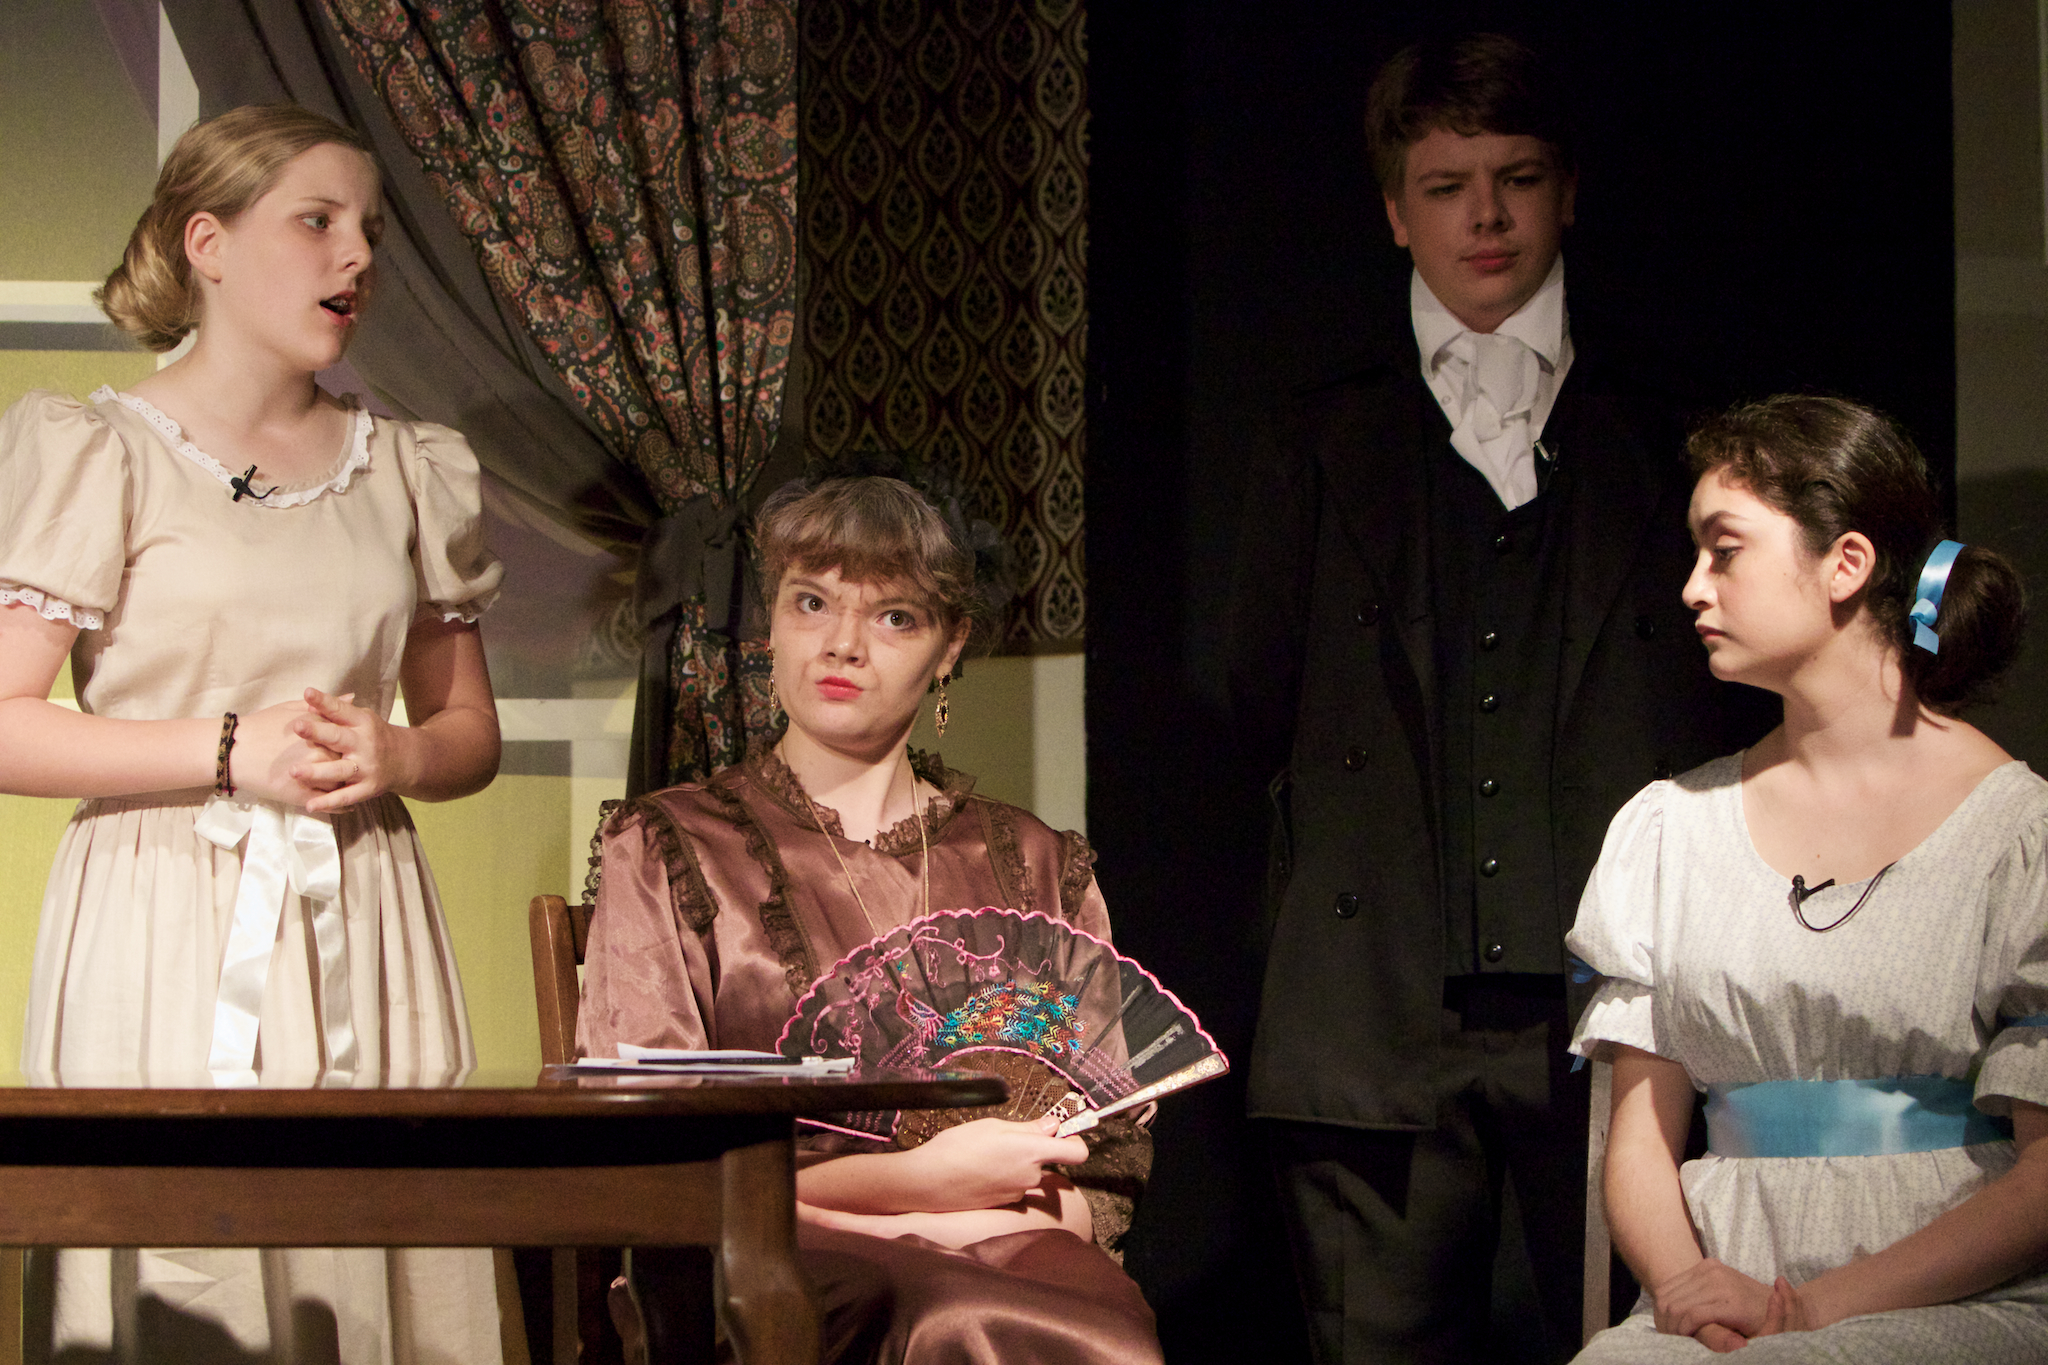
\includegraphics[width=\textwidth]{4_2_1_hl_e.jpg}}

\minor{Chiang Mai Circle of International School (CMCIS)}
 
As stated in a previous indicator, all  CMIS teachers attend the yearly Chiang Mai Circle of International School (CMCIS) conference.  As mentioned in the Research-Based Knowledge section, there is a different yearly theme. The 2014-2015 theme was The English Language Learner and saw four staff members provide presentations to local educators. The 2015-2016 conference saw the theme change to Technology in Education. One staff member presented during this conference. The number and quality of the presentations make it clear that CMIS is considered the instructional leader of international schools in northern Thailand. See \href{https://docs.google.com/a/cmis.ac.th/document/d/19oynokmtSbfGSbxQty71a1z3-sd_QGBngaBAVtS0W90/edit?usp=sharing}{CMIS CMCIS Presentations} for more information. 

\minor{Other Professional Development Opportunities}
 
Finally, CMIS Leadership would like to continue to emphasize that professional development happens in a variety of settings and environment.  Not only are early release Wednesdays or formal conferences examples of places where professional development happens. The following are examples of where professional development has been observed:
\begin{itemize}
\item Secondary offices are clustered by content and elementary workroom; 
\item Teacher Leadership Team and department meetings
\item School-wide functions, International Day \href{https://drive.google.com/drive/folders/0B0TYmzaZNi3fbnhzMzNNT3hKNm8?usp=sharing}{(2016)}, Thai day \href{https://drive.google.com/drive/folders/0B0TYmzaZNi3ffjNvUG85bU12TExQR1ZjMGtqcVZ1UFZrYWpwNHFGbDg2NFdrcDVmRmxkMmM?usp=sharing}{(2015)}, and National History Day \href{https://drive.google.com/drive/folders/0B0TYmzaZNi3fUkdpR1hLaDVaekk?usp=sharing}{(2016)};
\item Small, working groups organized for UbD planning;
\item Working groups on standards, interrater reliability, adoption. 
\item Individual meetings with the ES/MS principal
\item Instructional Rounds (2015, \href{https://drive.google.com/drive/folders/0B0TYmzaZNi3fbFVYTXpySHNDLUU?usp=sharing}{2016})
\item Cafeteria 
\end{itemize}

\minor{Professional Development Fund}

CMIS provides a Professional Development Fund for all teaching staff. Teachers receive 10000 baht per year to attend off- site professional development opportunities. Teachers are asked to submit a \href{https://docs.google.com/document/d/1zDwr8diiahPkrMQktXVF2-Us5eL-uVJDvdQLrbDNo8Q/edit}{Professional Development Application} which outlines how the professional development they plan to attend aligns with the CMIS Standards, their instructional round/deliberative practice goal, and how they plan to share the information with the staff. To date, since 2014, over 40,000 USD has been spent on teacher requested professional development. 

\minor{So what...}

Professional development at CMIS is a priority and CMIS Leadership will continue to fund the Professional Development fund. CMIS Leadership and Staff should continue to focus on reflective, genuine, deliberate teacher training, both in-house and outside. How the Leadership and Staff transition this professional development information to actual classroom practice and what accountability measures should be in place to ensure implementation of the concepts will be continue to be a goal in the near future. 
\end{findings}

\subsubsection{Challenging and Varied Instructional Strategies}

\indicator{The teachers strengthen student understanding and achievement of the learning outcomes, including targeted global competencies, through the use of a variety of instructional strategies that are selected on the basis of the learning purpose(s) and effectively engage students at a high level of learning. This includes the integration of multimedia and technology as appropriate and the linking of students’ experiences to the world.}

\prompt{Provide a range of examples from examining students working and their work that give insight to the degree to which all students are actively engaged in learning to achieve the academic standards and the schoolwide learner outcomes. This includes students demonstrating critical thinking, problem solving, knowledge, application and the development of a wide range of technological skills and global competencies.}

\begin{findings}

CMIS Staff use a variety of research-based instructional strategies, as well as practices that strengthen student understanding, consistently engage students, and provide learning tasks at a variety of complexities. 

Using instructional rounds, the CMIS Leadership Team used the Teach for Success (T4S) observation protocol to make interpretations about instructional strategies used at CMIS. See \href{https://docs.google.com/a/cmis.ac.th/spreadsheets/d/1ACz3l3DPUgIqRhmZ1LWk9RwVBjo0iLsbJAupJoic5Dg/edit?usp=sharing}{T4S Classroom Observation Protocol}, the \href{https://docs.google.com/a/cmis.ac.th/document/d/1cRvL50iIDvo8s1Gnxoczm82LhSVmEOvCrFksxzHD7ko/edit?usp=sharing}{T4S Data}, and \href{https://docs.google.com/a/cmis.ac.th/presentation/d/1LWASWS2DRPSgW6N4jZdZI4vuHiNOm3UoWzfGe91JdOs/edit?usp=sharing}{Instructional Rounds presentation} for more information. The data is separated into the following indicators:

\minor{Instructional Practices to Engage and Support All Students in Learning}
% (...effectively engage students)

This section describes how instruction at CMIS is delivered and/or supported within the classroom to engage all students in learning. Findings indicate that a majority of instruction is either teacher led (83\% of observed instruction) or student seatwork with teacher engaged (81\%).  Both practices are backed by research to be engaging for students if done in the context of the Teach for Success attributes.  See “so what…” section for areas of improvement. 

\minor{Student Engagement Throughout the Learning}
% (...effectively engage students)

This section describes how students at CMIS are engaged and the level of engagement. Data was collected two ways: charting teacher talk vs. student talk and the observing of the attributes of student engagement via the research provided by Teach for Success. Data indicate that overall, students engagement is high and that most teachers balance teacher talk vs. student talk. Of the Teach for Success engagement attributes, the CMIS teaching staff were observed Eliciting engagement, engaging all students at the same time, and maintaining engagement throughout the lesson most. See “so what…” section for areas of improvement. 

\minor{Level of Cognition}
% (...high level of learning)

This section describes the level of thinking reflected in the questions and activities from the lesson. Data indicate that CMIS provides students with an appropriate wave of complexity throughout the observational period. DOK 4 activities were observed least, followed by DOK 1. Most observed, which is to be expected, were activities representing levels of complexity at DOK 2 and 3. See “so what…” section for areas of improvement.

\minor{Instructional Practices Related to Standards, Curriculum, and Students}
% (... in learning to achieve the academic standards and the schoolwide learner outcomes)

This section describes how instruction is aligned to the CMIS standards, adopted curriculum, and the identified needs of students. Data indicate over half of the lessons observed ensured that Instruction was appropriate to grade level standard(s) (61\%) and the learning objective(s) communicated to all students (56\%).  Indicators in this section that had had high observation rates, included: Opportunities for interaction and discussion to elaborate between teacher/student and among students (89\%), regularly provides specific feedback to students on their output  (78\%) all teacher input, activities, questions and responses are related to objective(s) (78\%). See “so what…” section for areas of improvement. See “so what…” section for areas of improvement.


\minor{Instructional Practices to Enhance and Extend Learning}
% (...strengthen student understanding and achievement of the learning outcomes...)

This section describes types of support provided by the CMIS Teaching Staff to enhance and extend learning for all students. Data indicate that teachers use the Questions, cues, and/or advance organizers practice (26 times observed) most, followed by the Homework and/or practice (18). Both practices, if observed with the research-based attributes,  are effective in enhancing and extending learning. See “so what…” section for areas of improvement. Note Taking (11) and Identifying Similarities and Differences (11) were the next most used practices.  See “so what…” section for areas of improvement.
                
\minor{Creating and Maintaining Effective Learning Environments for 
Student Learning}
% (...strengthen student understanding and achievement of the learning outcomes...)

This section describes how the CMIS Teaching Staff use the classroom environment to support student learning. Findings include: observing a Climate of fairness, caring, and respect that is maintained by the teacher (100\%), Standards for behavior are maintained by teacher (100\%), and 
Reinforces effort and/or provides recognition (83\%). See “so what…” section for areas of improvement.

\minor{Student Work}

Samples were requested from departments. Each sample was analyzed to determine “...the academic standards and the schoolwide learner outcomes” as well as rigor (i.e. using DOK measurement). See Student Sample folder for \href{https://drive.google.com/drive/folders/0ByVFfrm0zfolVGJzdXpvLV9reVk?usp=sharing}{K-5} and  \href{https://drive.google.com/drive/folders/0ByVFfrm0zfolMkF5aThoSzZxa1E?usp=sharing}{6-12}. 

\minor{Using Authentic Audiences}

CMIS Leadership and Teaching Staff have also continued to address student understanding and achievement, as well as engagement and rigor by encouraging instruction and assessment by focusing on using authentic audiences. According to Levy, “The most effective way to engage  students in learning is to create an authentic audience, giving them a sense that someone else (besides teachers and parents) cares about their work. They need to have a vision of a product that matters. They need to learn content and develop skills to complete the product.” (2008)  Events organized by the CMIS Teaching Staff have included the use of authentic audiences as well as addressing global competencies.  CMIS music, drama, and dance events are held at least once a semester and are consistently some of the most attended events of the year. CMIS sporting events, especially the many interscholastic tournaments held on site, attract a sizable audience to watch students compete. 

{\centering
\includegraphics[width=\textwidth]{4_2_1_hl_g.jpg}}

National History Day (NHD), for example, asks students to choose a historical  topic that is aligned with the yearly theme. During our own on-site History Day students present their product and are interviewed by teams of teachers, parents, and community members who provide feedback and encouragement

The 8th Grade Science Fair also gives an opportunity for students to share their experimental questions and finding to groups of parents and community members. 

\href{https://drive.google.com/drive/folders/0Bwo-i12FeO0rVmRhaGd4QlE5ek0?usp=sharing}{Model United Nations (MUN)} is another example of students engaged in work that includes an authentic audience and global competencies. CMIS MUN were successful during the 2015-2016 year and will host the regional competition during the 2016-2017 school year. 

History Bowl and Bee provided students with an opportunity to test their knowledge of world history through a competitive format. 
During the 2017-2018 school year, the CMIS Teaching Staff would like to expand our focus on using authentic audiences by implementing the Google International Science Fair and Junior Achievement’s International Trade Challenge and  Company Program of the Year programs. 

\href{https://drive.google.com/drive/folders/0B0TYmzaZNi3fMGp2X0xiMk52alk?usp=sharing}{National Honor Society} and the \href{https://drive.google.com/drive/folders/0B0TYmzaZNi3fSVVEd0VWTkcwVU0?usp=sharing}{CMIS Student Council} are other non-classroom opportunities that exist for students to engage with authentic audiences and address global competencies. 

\minor{So what...}
 
The CMIS Teaching staff effectively engage students in high levels of learning. Though the data indicate that CMIS is addressing this indicator, there are areas of improvement; CMIS Leadership understands that the methods that were observed the fewest might be occurring outside of the observation window. In order to address this, CMIS should utilize the Teach for Success observation protocol more consistently and frequently. Other areas of growth by indicator include: 

\minor{Instructional Practices to Engage and Support All Students in Learning}

% (...effectively engage students). 
The CMIS Teaching Staff has expressed a great deal of interest in determining levels of engagement in their classrooms, differentiating between engagement and compliance, and utilizing effective engagement strategies during the instructional rounds period. Resources and time should be devoted to practicing two methods to engage and support learners that were observed the least: active learning and facilitating student conversation. 

\minor{Student Engagement Throughout the Learning}

% (...effectively engage students)
Eliciting engagement, ensuring that all students were prompted to be engaged, and maintaining engagement were indicators that were observed frequently, making engagement mandatory is an area that could be explored for improvement. 

\minor{Level of Cognition}

% (...high level of learning) 
CMIS Teaching Staff should continue to maintain and monitor a variety of levels of complexity as the data shows. See section entitled: Evidence of Results based upon Challenging Learning Experiences for explanation of DOK levels. 

\minor{Instructional Practices Related to Standards, Curriculum, and Students}

% (... in learning to achieve the academic standards and the schoolwide learner outcomes)
CMIS is currently addressing the indicators that deal directly with stating the objective and the standards: Instruction was appropriate to grade level standard(s) (61\%) and the learning objective(s) communicated to all students (56\%) by asking the Teaching Staff to post or state the objective during each lesson. Two indicators that were observed the least: 
Key vocabulary emphasized and Use of scaffolding techniques to assist/support student understanding could be areas that the staff focus in the future. 

\minor{Instructional Practices to Enhance and Extend Learning}

% (...strengthen student understanding and achievement of the learning outcomes...)
The research-based instructional practices that were observed the fewest times could be possible professional development topics for next year: 
Summarizing observed 3 times, Generating and/or testing hypotheses observed 3 times, Cooperative learning 4 times, and the use of  Nonlinguistic representations 6 times. 

\minor{Creating and Maintaining Effective Learning Environments for 
Student Learning}

% (...strengthen student understanding and achievement of the learning outcomes...)
The CMIS Teaching Staff truly and genuinely create and maintain classroom climates of fairness, caring, and respect. Effective standards for behavior are also maintained by teacher as the data indicate. 
\end{findings}

\subsubsection{Technological Integration}

\indicator{Teachers systematically integrate technology within the school so that all students develop a wide range of technological skills.}

\prompt{Comment on the integration of technology within the school so that all students develop a wide range of technological skills.}

\begin{findings}
CMIS Teaching Staff use technology consistently and frequently. Data collected during instructional rounds and through staff survey indicate that computer technology is an important part of the instructional process in grades K-12. 

\minor{Technology Integration}

CMIS students in grades 6-12 participate in a 1:1 Chromebook program. CMIS Leadership implemented this program in the 2013-2014 school year to facilitate the integration of the \href{https://drive.google.com/a/cmis.ac.th/file/d/0ByVFfrm0zfolakw5TUstQ1ZrVDFCRjR1d1JQSUpQbkZaVDBr/view?usp=sharing}{International Society for Technology in Education (ISTE)} in all middle and high school classes. These research-based standards help empower students to take more control of the learning and progress and encourage inquiry based instruction. 

{\centering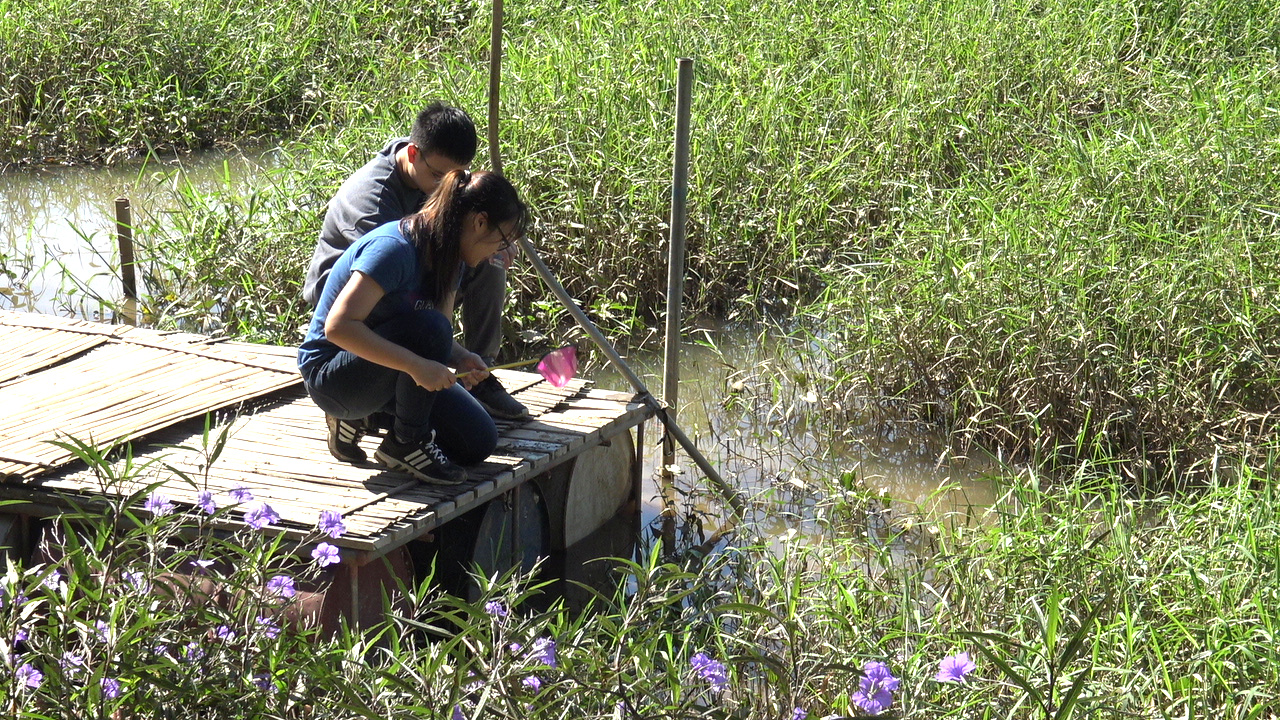
\includegraphics[width=\textwidth]{4_2_1_hl_h.jpg}}

\textit{Students recognize the rights, responsibilities and opportunities of living, learning, and working in an interconnected digital world, and they act and model in ways that are safe, legal and ethical.} For example, CMIS students have frequent digital citizenship lessons to guide them to make responsible digital decisions in the elementary computer classes in elementary and middle school. Starting in the 2016-2017 school year, students have been assigned to electronic classrooms where they will receive additional digital citizenship modules (e.g. plagiarism, piracy, and cyber bullying). These learning modules will be embedded in their Communication Group curriculum. Please see \href{https://docs.google.com/a/cmis.ac.th/document/d/1TRVPFDs7fyAcRDXcuaha4E4jx53zryfG155vC8Sd-sk/edit?usp=sharing}{Plagiarism Mini Lessons} and \href{https://docs.google.com/a/cmis.ac.th/document/d/1xBZgw3vpW2UPOx_kEWC0oCk34H1OWDri1o4hcQS5VQc/edit?usp=sharing}{Digital Citizen Websites} 

\textit{Students critically curate a variety of resources using digital tools
to construct knowledge, produced creative artifacts and make
meaningful learning experiences for themselves and others.} For example, CMIS students create online peer assessments, peer evaluations, and projects-large and small (e.g. National History Day in which CMIS has a institutional account for \href{http://www.noodletools.com/}{Noodletools}). Additionally, CMIS elementary school students participates in the yearly Hour of Code initiative. This program exposes students to basic coding concepts and demonstrates creative problem solving models. 

\textit{Students use digital tools to broaden their perspectives and
enrich their learning by collaborating with others and working
effectively in teams locally and globally.} A CMIS middle school teacher partners with a school in Kuwait as her students are studying that region of the world.  These CMIS students  created three Vlogs to foster cross-cultural understanding.  They are also using the Screencastify app to make the videos.

\textit{CMIS Students use collaborative technologies to work with others, to examine issues.} For example, high school chemistry students are reading the informational text, \textit{Stuff Matters} and have organized a Google Hangouts session with the author to discuss topics related to material science. See \href{https://docs.google.com/a/cmis.ac.th/document/d/15hsNNTonRewyDmMCelG2aVxweUJhej15h627tCAQBXg/edit?usp=sharing}{Technology Snapshots} for other anecdotes on how CMIS teachers and students use computer technology. 

\minor{Embedded Integrated Technology Standards}

Starting in the 2016-2017 school year, all teacher created Understanding by Design units have a section which asks the designer to embed the International Society for Technology in Education (ISTE) standards. Teachers will be encouraged to reflect on previous plans to embed ISTE standards during the 2017-2018 year.  

\minor{Technology Integration Professional Development}

The CMIS Teaching Staff have been provided with a number of opportunities to assist in integrating technology. Middle and high school teachers have participated in two Google Apps for Education Conferences(G-Suite) in 2013 and 2014, CMCIS Technology Conference (March, 2015), Grace International School IT PD Day (November 2015) , Lanna International School Technology Weekend (2015). Additionally, CMIS has devoted financial resources to allow interested teachers to complete the Google Certified Educator Level 1 certificate. 

\minor{Teacher Technology Chromebook Survey}

data indicate that 6-12 teachers utilize the Chromebook to facilitate student collaboration and communication and to encourage digital citizenship with the most frequency. In the collaboration and communication questions, all teachers surveyed  indicated that they had students “Interact, collaborate, and publish with peers, experts, or others employing a variety of digital environments and media” in many or most classes. In the digital citizenship question over 75\% of the teachers responded that they use the Chromebooks in many or most classes to: “Exhibit a positive attitude toward using technology that supports collaboration, learning, and productivity” and to “Advocate and practice safe, legal, and responsible use of information and technology”. See Chromebook \href{https://goo.gl/forms/QsbCBzfO0psqcbXQ2}{ISTE Survey}, Chromebook \href{https://goo.gl/forms/1mda4plq0tzQiTed2}{Student Survey}, and \href{https://docs.google.com/a/cmis.ac.th/presentation/d/1xmLAJD96klLrjiBPwCoOMoKmbclYqpIMWaifytzFMgk/edit?usp=sharing}{Chromebook Surveys - Student and Teacher Responses} for more information. Also, see the so what… section for areas of improvement.

\minor{Instructional Rounds}

Observational data from the Instructional Rounds sessions between September and November 2016 indicates that most instruction in grades 6-12 utilized the student’s Google Chromebook in various ways. Students were observed creating and revising work on a shared Google document, having synchronistic discussions,  using Slide presentation to facilitate reciprocal teaching, accessing Google Classroom, analyzing data sets, and researching were the most observed applications of the Chromebook. See \href{https://drive.google.com/drive/folders/0ByVFfrm0zfolUkxUSmg2VGJCTGc?usp=sharing}{Instructional Rounds Data} for archive.

\minor{So What...}

Many CMIS Staff members use computer technology to facilitate instruction skillfully and CMIS Leadership understand that true technology integration is still a work in progress. Based on the limited data on how teachers use the Chromebooks, two indicators scored low with respondents stating they do not use the Chromebooks “at all”  to: Collect and analyze data to identify solutions and/or make informed decisions and Use multiple processes and diverse perspectives to explore alternative solutions. Resources and time could be spent on coaching teachers on how to implement and embed those indicators in instruction.

{\centering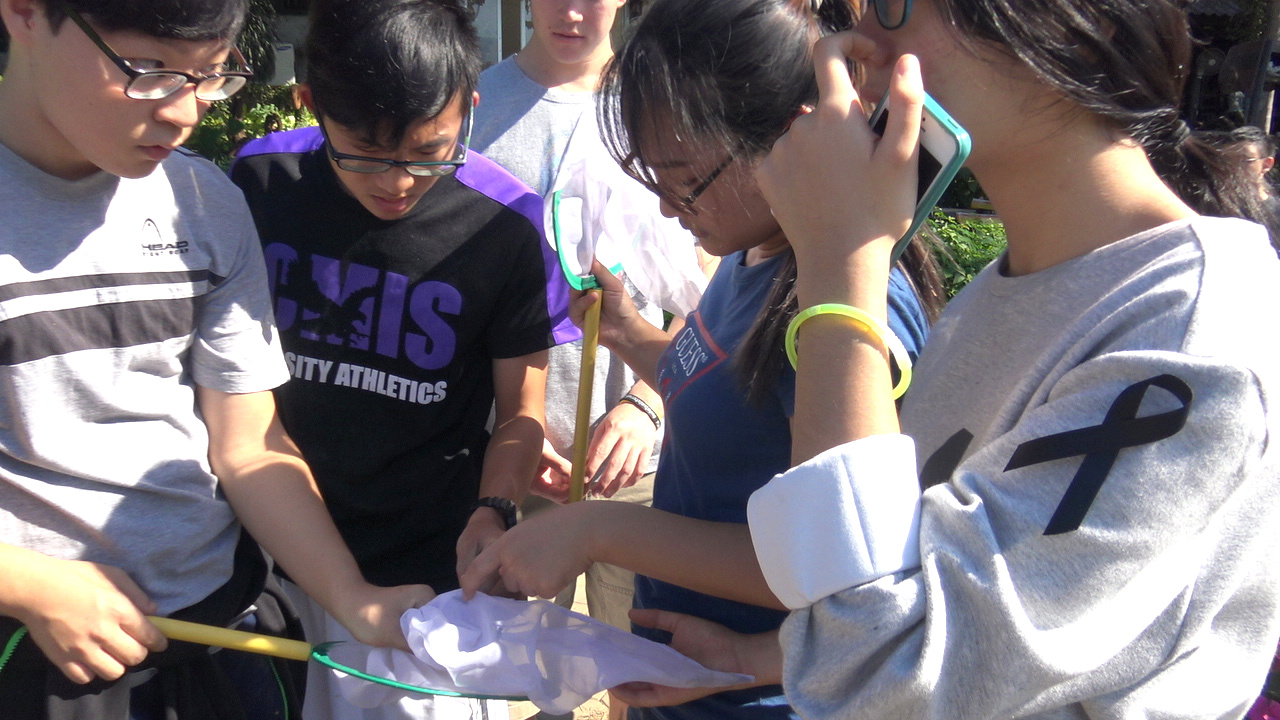
\includegraphics[width=\textwidth]{4_2_1_hl_i.jpg}}

Time and resources should be devoted to creating a CMIS Technology Vision, which should include a common understanding of how technology should be integrated systematically. 

Finally, CMIS Community Survey indicated areas of for improvement in regards to teachers having adequate IT support and resources. The CMIS IT Department will continue to address these areas for improvement. 
\end{findings}

\subsubsection{Evidence of Results based upon Challenging Learning Experiences }

\indicator{Students working and their work demonstrate critical and creative thinking, problem solving, knowledge attainment, and application skills.}

\prompt{Comment on the student work and how it demonstrates critical and creative thinking, problem solving, knowledge attainment, and application skills.}

\begin{findings}
Student work and observations of students working indicate that CMIS provides students with a balance of challenging learning experiences as well as activities and assignments that require practice with fluency and application.  

\minor{Depth of Knowledge }

In order to measure if students were working demonstrate critical and creative thinking, problem solving, knowledge attainment, and application skills, CMIS Leadership and Teaching Staff used the  \href{https://drive.google.com/a/cmis.ac.th/file/d/0ByVFfrm0zfolNVJmeEJwcHUxbjg/view?usp=sharing}{Depth of Knowledge (DOK)} tool to measure the rigor of the  instructional task. 

Webb (1997) developed a process and criteria for systematically analyzing the alignment between standards and standardized assessments. Since then the process and criteria have demonstrated application to reviewing curricular alignment as well. This body of work offers the Depth of Knowledge (DOK) model employed to analyze the cognitive expectation demanded by standards, curricular activities and assessment tasks (Webb, 1997). Please see \href{https://docs.google.com/a/cmis.ac.th/document/d/1cZlDn-POZCJs2XZ1SLF-CL_DtiO4GscppQ71QZJtFGg/edit?usp=sharing}{Table 10} reflects the version of the model CMIS used during our analysis of  students’ working along with the WASC FOL terms used in the indicator. 

The observers during instructional rounds were asked DOK when analyzing student work. Between September and November, 2016, data was recorded from 36 classrooms with a total of 53 different learning tasks observed; 41 of the 53 tasks were either Level 2, 3, or 4. This data initially indicates that the CMIS Teaching Staff provides an appropriate mix of complexity levels appropriate for their grade levels and contents. See \href{https://docs.google.com/a/cmis.ac.th/document/d/1cRvL50iIDvo8s1Gnxoczm82LhSVmEOvCrFksxzHD7ko/edit?usp=sharing}{T4S Data} for more information. 

Though CMIS will  continue to emphasize looking at student work more consistently and with more guided structures, the time we have in department meetings and divisional meetings reveal a appropriate balance of DOK levels. Some descriptions of student work that are at a DOK 3 and 4 level include: 
\begin{itemize}
\item High school science engaging their students in the development of a series of experiments to test their hypothesis.
\item Middle school physical education assigning an exercise in which the students create their own game, develop the rules, and teach it to their peers. 
\item Kindergarten students sequencing a series of life events from oldest to most recent and describe verbally how we know about these events and decide which event is most important. 
\item Eleventh grade ELA students writing an argumentative essay using a literary criticism “lens”. Students then have to respond to the essay from the opposite “lens” 
\item Third grade students devise a plan to use the distributive property of multiplication to find the number of toys in a toy shop in a large array, and then again to find the total price for all of the toys.
\item 7th grade students asked to develop a string of PEE sentence structures to provide evidence and justification of thematic and characterization elements from the short story Old Man from the South by Roald Dahl. 
\end{itemize}

See Student Sample folder for \href{https://drive.google.com/drive/folders/0ByVFfrm0zfolVGJzdXpvLV9reVk?usp=sharing}{K-5} and  \href{https://drive.google.com/drive/folders/0ByVFfrm0zfolMkF5aThoSzZxa1E?usp=sharing}{6-12} for student samples of DOK levels and individual \href{https://docs.google.com/a/cmis.ac.th/document/d/1kL1VjwfuMMa7NaWmwUrEah1BM-jJRmLAd4VJzR3HoPs/edit?usp=sharing}{UbD Unit} plans for other assignments measured for DOK 

\minor{So what...}

data indicate that CMIS students are provided multiple and consistently challenging learning experiences in all grade levels and content areas. Further time and resources to look at student work more frequently would be beneficial data to continue to maintain and monitor instructional, curriculum, and assessment decisions.  
\end{findings}

\subsubsection{Student Understanding of Performance Levels}

\indicator{The students know beforehand the standards/expected performance levels for each area of study.}

\prompt{Examine and evaluate the extent to which students know the standards/expected performance levels before beginning a new area of study.}

\begin{findings}
CMIS Teaching Staff communicates the expected performance levels based on adopted standards for each area of study and grade level in a variety of ways:

\minor{Communication of General/School Wide Performance Levels}

Teachers in grades 3 through 12 are required to review all relevant sections of the \href{https://drive.google.com/file/d/0B8vOjwyFoCioQ2tNak04WGd3Mm8/view?usp=sharing}{CMIS Planner} that explain expected performance levels with their students at the beginning of the year. The relevant section entitled, Reporting Academic Progress (p. 16-17), details the elementary academic reporting policy and report card information. Middle and high school information begins on page 17 and contains information relating to Powerschool use and the grading scale. Time is provided for 9-12 teachers to review the CMIS Planner during the first Communication Period. 

\minor{Syllabus/class information}

Many teachers in grades 6 through 12 provide their students with a syllabus. At a minimum, each syllabus is required to contain the following elements: course objectives/learning outcomes which are aligned to the CMIS adopted standards, attendance policy, late work policy, grading scale, assignments with points possible or percentage grade weight. See \href{https://drive.google.com/drive/folders/0ByVFfrm0zfolNmdnMzU2S2xRSWs?usp=sharing}{CMIS Syllabus} folder for examples. 

Other means of communicating school-wide performance levels include parent/teacher conferences and back-to-school night.  

\minor{Communication of Specific Standard Aligned Performance Levels}

All CMIS Teaching Staff use a combination of grading criteria, answer keys, and rubrics in varying frequency to communicate mastery or non-mastery of performance levels based on adopted standards. See Student Sample folder for \href{https://drive.google.com/drive/folders/0ByVFfrm0zfolVGJzdXpvLV9reVk?usp=sharing}{K-5} and  \href{https://drive.google.com/drive/folders/0ByVFfrm0zfolMkF5aThoSzZxa1E?usp=sharing}{6-12} for teacher samples of assessments aligned to the standards. 

There are also a number of other methods the CMIS Teaching Staff use to communicate specific standards aligned performance levels to students. CMIS Teaching Staff use Google Apps,  especially Google Classroom and Google Sites, blogs, and Powerschool to communicate performance levels to students and parents.

\minor{Communicating Performance}

Beginning in the 2016-2017 academic year, CMIS Leadership will request that all teachers communicate the learning goal or standard. Teachers will have flexibility on how to communicate as well as how to implement this practice. First, the CMIS Teaching Staff can decide if they communicate the academic standards, using student friendly language, to the students or if they would like to develop or have the students develop academic goals  based on the standards or essential  question. Secondly, Teachers can post or display the goal or standard, explicitly and verbally state them, or ask the students to refer to them before, during, or after instruction. Initial communication of the standard or goal and consistent  and regular reference to them will also be emphasized. 

During instructional round sessions between September and November, 2016 data was collected regarding students ability to explain the objective of their work. Data indicated that positive student responses to the questions: “Can you explain what you are doing?” or “What are you doing” was high. 12 of 14 students asked this question could answer completely and accurately. 

It is clear to CMIS is the research suggesting that communicating the learning goal or standard has a positive effect to enhance learning (Marzano, 2007). Effective standards based instructional practice requires the teacher to provide students with the instructional goal as part of the lesson; as a point of departure (Saphier, 1997).  Finally, as Hunter found, students usually will extend more effort and consequently increase their learning if they know what it is they will learn and why it is important to them (1982). 

Instructional rounds, informal walk throughs, and formal observations will continue to be used to determine if the practice is being implemented successfully.  Practitioner reflection of the practice in May 2017 will be scheduled to determine if the implementation had a positive effect on learning and achievement. See \href{https://docs.google.com/a/cmis.ac.th/document/d/1cRvL50iIDvo8s1Gnxoczm82LhSVmEOvCrFksxzHD7ko/edit?usp=sharing}{Teach for Success Data CMIS September - November 2016} for more information. 

\minor{Student Understanding of the Performance Levels and Standards}

When asked if they knew of how they were graded in their classes a vast majority of the high school students responded with an answer that outlined tests, homework, participation, quizzes, and GPA. This data suggest that they have an understanding of grades, not necessarily of performance levels or standards. 

\minor{So what...}

Though, CMIS Students know what is expected of them and the CMIS Teaching Staff communicates expectations in a number of ways, the data also indicates that students equate performance levels with letter grades. When interviewed about if they know the how their grades are determined, a vast majority of students state that the grade is based on homework, activities, tests, labs, and projects--though this is accurate, it is also superficial as they have less awareness of performance levels based upon rubrics and formative assessment. CMIS should continue to implement the posting or verbally stating of the objective and/or standards to increase student understanding of their class or course performance levels and standards beyond letter grades and/or percentages. 
\end{findings}

\subsubsection{Student Perceptions }

\indicator{ Interviews and dialogue with representative students inform the degree to which learning experiences are relevant in preparing students for college, career, and life.}

\prompt{Using interviews and dialogue with students, evaluate the extent to which students understand the expected level of performance based on the standards and the schoolwide learner outcomes. Evaluate the effectiveness of the student-teacher interaction based on student feedback.}

\begin{findings}

Student survey data and interview responses indicate that a majority of the students feel that their learning experiences are relevant in preparing students for  college, career, and life. 

End-of-year student survey data indicate that of the questions that relate to learning being relevant to college, career, and life such as, “CMIS helps students become responsible”, “My teachers are helping me to become a better student”, and “My teachers set high standards for learning in their classes” a majority (over 51\%) of students respond favorably by agreeing or strongly agreeing with the statement.  See \href{https://docs.google.com/document/d/1DO6UYDibCyF0wjGx1Pi7tgKJYMqpfjzTcICvsf8UUWM/edit}{Figure 12} and Student surveys for  \href{https://docs.google.com/a/cmis.ac.th/forms/d/1EbMhxXKv9boAXmuwqmldZCbHKNY-aREq56IW2N-eviI/viewanalytics}{2013-2014}, \href{https://docs.google.com/a/cmis.ac.th/forms/d/1qbAnJ69O0ZRUPmBFvQaglObvnyoUkVd4hQiyaAFO7_I/viewanalytics}{2014-2015} and \href{https://docs.google.com/a/cmis.ac.th/forms/d/1n7vFCQbPQmF6pEPJKPBsu4rzdiW4KQ_DrBcjTMUbLH4/edit?ts=587d7b50#responses}{2015-2016} for more information. 

Other data indicate the same. When asked explicitly, “How is your learning at CMIS relevant to your future goals?” a majority of the high school students stated that learning was relevant.  A snapshot of student comment include: 

``CMIS is giving me the basic skills I need to be able to pursue a successful career and thrive in life'' -10th grade student
 
``I find learning at CMIS more like a tool to guide me where I want to go rather than taking me there.'' - 9th grade student 

``Learning at CMIS give me opportunities to challenge myself in different field to figure out what I am really interest in or passionate about'' - 11th grade student

``CMIS prepared me for university by  providing me with opportunities  to take advanced classes'' -12 grade student 

\minor{So what...}

CMIS is data rich with current student perceptions. Though the collection and capturing of current student perception data is thorough, more time could be devoted to analyzing the gradual down tick in some data and post graduation readiness data- this data is where CMIS feels it can accurately respond to this indicator. Also, greater time should be spent on modifying the student perception questions to align with more current goals.  
\end{findings}

\subsubsection{Student Needs}

\indicator{ Teachers address student needs through the instructional approaches used.}

\prompt{ How do teachers address the variety of ways in which students learn and their individual needs through instructional approaches appropriate for the subject?}

\begin{findings}
As detailed in the Accessibility of All Students to Curriculum section, the CMIS Teaching Staff provide a variety of access points for students to engage with the curriculum. Through the use of differentiation practices in content, process, product, and learning environment provided by some teachers, the CMIS Teaching Staff addresses the majority of CMIS student needs. 

\minor{Schoolwide Student Needs }

However, there are specialized, individual, and school-wide students needs that the CMIS Teaching Staff addresses with a high degree of efficacy. 

\minor{English Language Learners }

For those students who have student needs that involve English language learner (ELL) or special support services (both for learning and/or behavior), CMIS Leadership has made changes in the procedures to ensure that services are provided based upon quantitative and qualitative data. This data is collected from an age appropriate, research-based measurements or  tests.  For ELL, this is the WIDA created W-APT Assessment administered by our Student Support department. For those who might benefit from special education services, CMIS Leadership uses a combination of child study, classroom teachers notes, outside advocates, and previous school reports to make placement decisions. Other research-based measures used to make instructional decisions based on student needs are the DRA and  Early Screening Inventory (ESI). Elementary teachers use the DRA data to make instructional decisions and identify skills which require further focus in areas such as oral fluency and comprehension. Data also indicates that progress monitoring is routine. For student support, CMIS Leadership and Student Support team have emphasized well written IEP reports and well organized IEP meetings to ensure accurate placement and appropriate interventions. 

\minor{Interventions}

For all students, including ELL and student support students, a majority of the CMIS Staff utilize standard Tier 1 processes to meet student needs such as differentiation of content, process, product, affect, learning environment, classroom discussion and opportunities to speak and listen, use of feedback and formative assessment, student choice, strategic accommodations (e.g. preferential seating), and the use of  Gardner’s Multiple Intelligences for planning and instructional adjustments. 

{\centering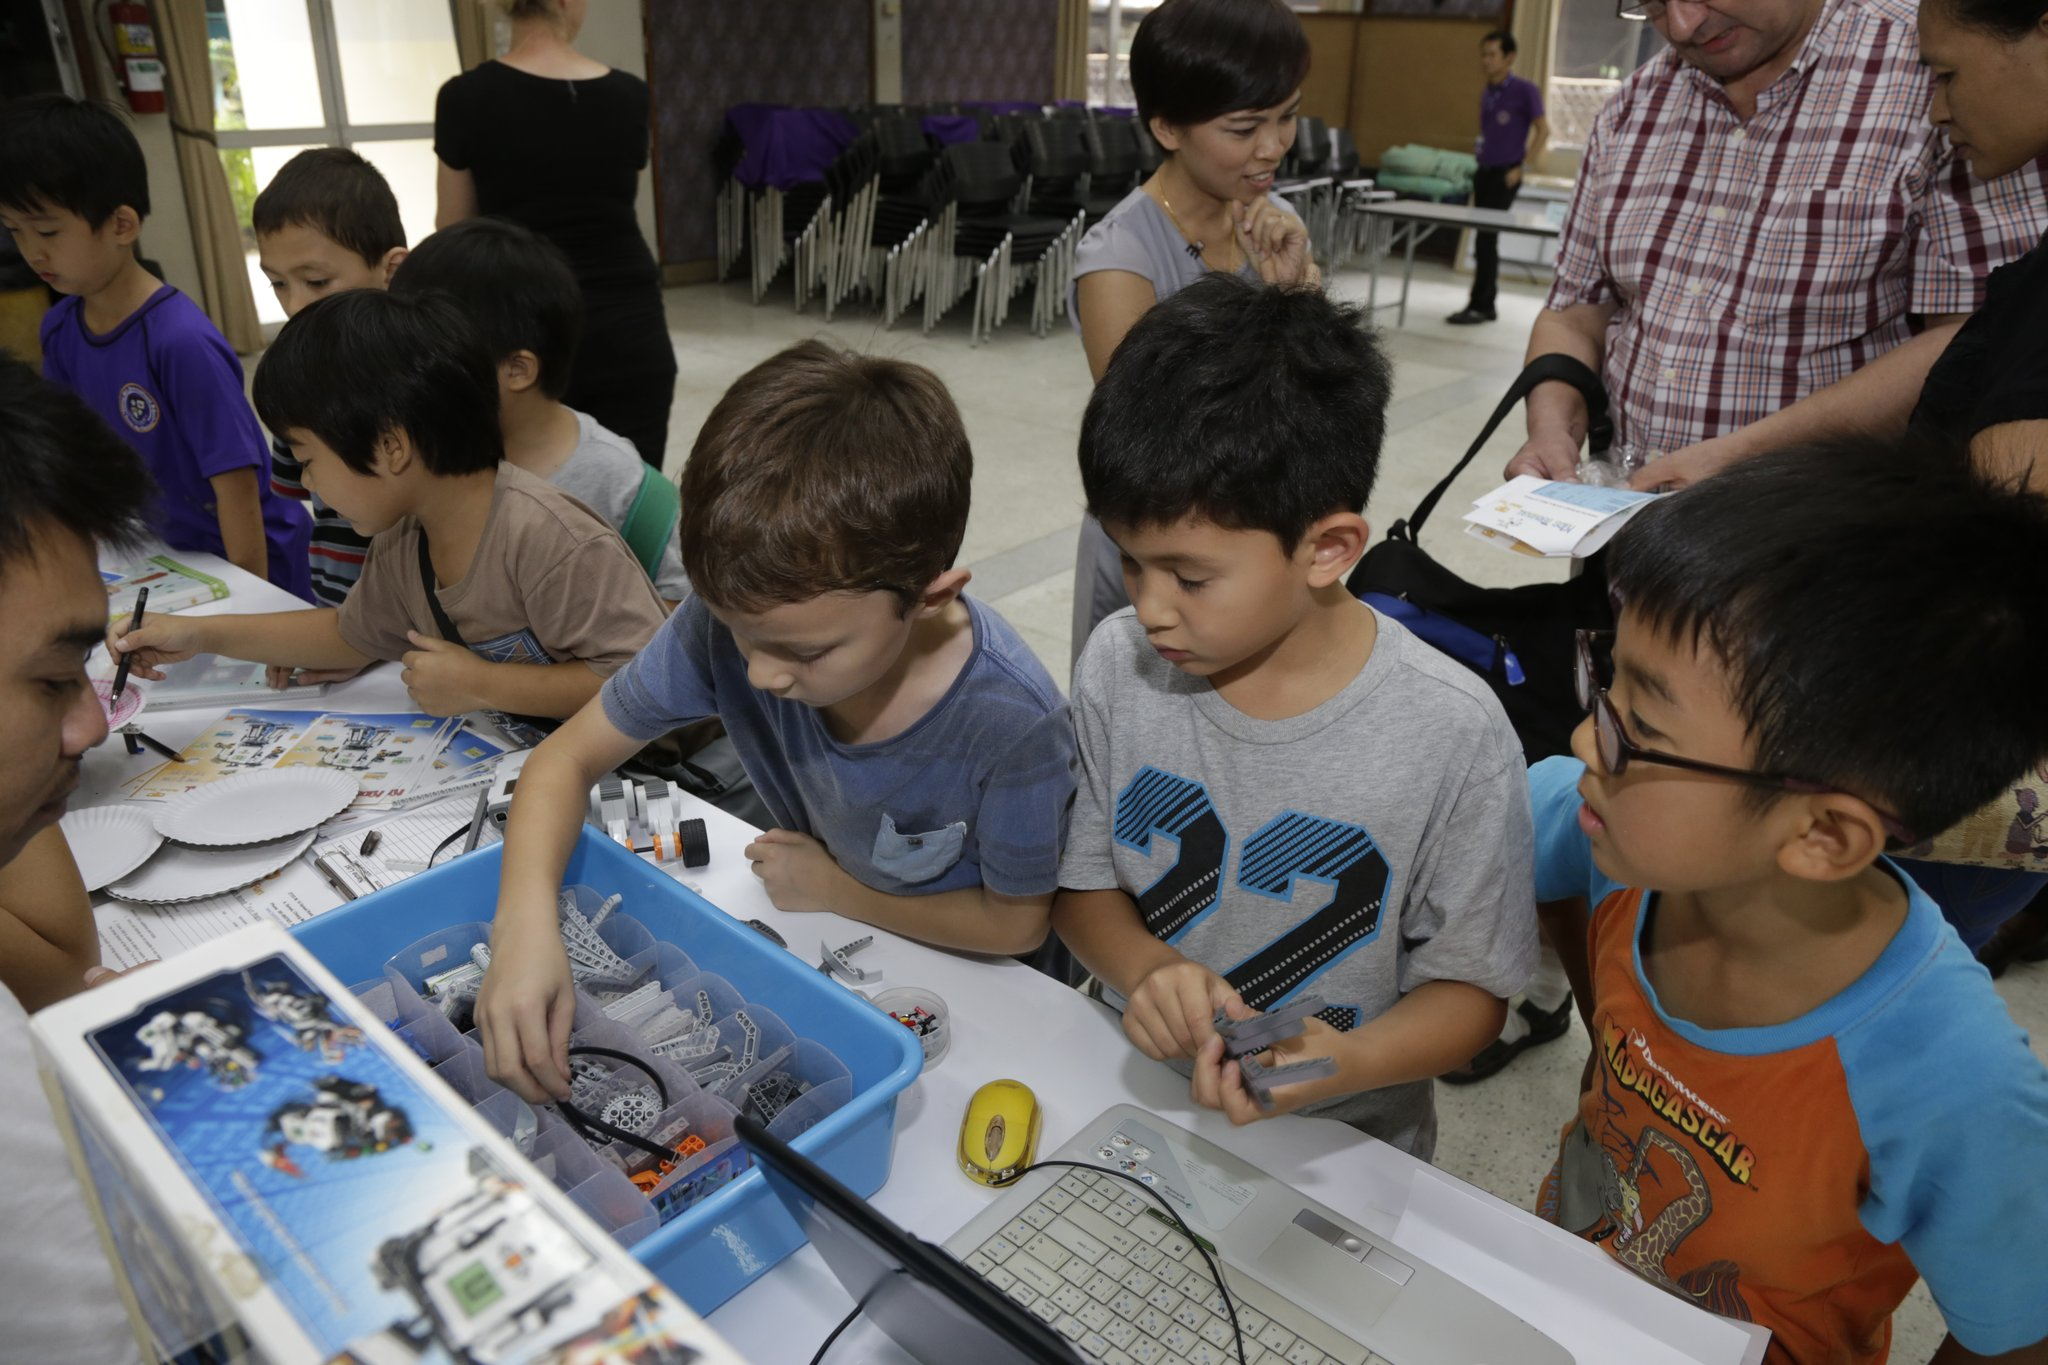
\includegraphics[width=\textwidth]{4_2_1_hl_j.jpg}}

In the elementary division, some teachers effectively meet student needs by organizing homogeneous small groups based on skill deficit. CMIS  recognizes that the level of evidence for this intervention is considered strong (i.e. consistent evidence supporting this practice as an intervention) and is directly related to improved student achievement. 

\minor{Student Perception Survey Data}

Student survey evidence indicates that 50\% of CMIS students agree or strongly agree that they are “in charge”  of what they learn on the last student survey, which is an increase of 7\% from the previous two years. Alternately, the percentage of students who feel that they are not “learning how [they] learn best” has increased the past year. These two indicators were chosen as they most align with addressing individual student needs. See Table 12 for more information. 

\minor{Teach for Success Observational Data }

The instructional rounds scheduled between September and November, 2016 provide a great deal of observational data on varied instructional approaches. Table 6 briefly describes the instructional approaches used in one week of instructional rounds, September 5 to September 9, 2016. Though a snapshot of only one week, analysis of the data suggests CMIS teachers use a variety of instructional approaches to address student needs. 

Other instructional approaches used can be found on the Instructional Strategies Snapshot. 

\minor{So what...}

The observational and perceptual data indicate that CMIS is meeting student needs by using a variety of methodologies. Greater time and resources could be devoted to developing and planning more strategic interventions and enrichments based on data and embedded into the unit planning (e.g. disengaged, high achieving, struggling students). Of the indicators from the student survey that could be targeted for improvement, student perceptions of how teachers are able to meet their needs is one that could use additional time and resources to address. 
\end{findings}

\subsubsection{Student Use of Resources}

\indicator{Students use resources for learning beyond the limits of the textbook such as effective use of collaborative activities, technology, library/media resources and community resources and information from various cultures and languages.}

\prompt{To what extent do students use resources for learning beyond the limits of the textbook such as effective use of technology, collaborative activities, and community resources?}

\begin{findings}
CMIS Teaching Staff use a variety of resources to ensure collaboration, technology, and community resources. 

Generally, the elementary classrooms contain a variety of resources, including a book library, math manipulatives, projector, screen, a computer, document cameras, educational games; some classrooms have a tablet and dongle to project the tablet. 

Tables and desks can be rearranged to facilitate student discussion, varying learning styles, and effective management

Collaborative tools include Google Classroom, Google Apps (Docs, Slides, Forms). CMIS utilizes many community resources, such as and Rotary Club volunteers for student judging, guest speakers, parent helpers, and consular employees. 

Students regularly check out books from the library both for research purposes and  because they are interested in a topic or for free reading.  For example, grade 5 has students using the library for research assignments every quarter. 

Instructional/Content resources are varied and rich. The examples below are in no way represent an exhaustive list of resources the CMIS Staff uses to go beyond the textbook. 
 
\minor{Science}

\href{https://pogil.org/}{Process Oriented Guided Inquiry Learning}, non traditional/informational text- Stuff Matters, \href{http://sciencecases.lib.buffalo.edu/cs/}{National Center for Case Study Teaching in Science}, \href{https://docs.google.com/a/cmis.ac.th/document/d/16TR92UNODi6qAM_vZkqFmqV_NGde5JCabfIoimXw8EM/edit?usp=sharing}{FOSS Science Modules}, Kahoot, \href{http://www.ck12.org/}{CK12}

\minor{Social Studies}

\href{http://www.gilderlehrman.org/programs-exhibitions/for-students}{Gilder Lehrman Institute of American History}, \href{http://www.digitalhistory.uh.edu/}{Digital US History},  \href{https://www.docsteach.org/}{DOCSTeach}, \href{http://nhd.org/}{National History Day}, \href{http://www.mindsparks.com/c/mindsparks.web?nocache@1+s@wS_b7B8iF3AX2}{MindSparks}, Opposing Viewpoints series, \href{http://www.welkerswikinomics.com/home.html}{Welker's Wikinomics}, Scoop It, Facing History, Facing Ourselves, Quizlet 

\minor{English/Language Arts}

\href{https://newsela.com/}{NewsELA}, \href{https://www.gutenberg.org/}{Project Gutenberg}, Ted Ed, No Red Ink, Flocabulary, EdPuzzle, \href{https://www.learninga-z.com/}{Learning A-Z}, \href{https://www.raz-kids.com/}{Raz Kids}, \href{http://www.abcteach.com/}{abcteach}, CK12, National Geographic Online 

\minor{Mathematics}

\href{https://www.illustrativemathematics.org/}{Illustrative Math}, \href{https://www.engageny.org/}{EngageNY}, NCTM, 

\minor{Student Support}

\href{http://www.wilsonlanguage.com/programs/wilson-reading-system/}{Wilson Reading System} 

\minor{World Language}

Confucius Institute at CMU, Chinese Consulate in Chiang Mai , Duolingo
\href{http://www.bbc.co.uk/languages/}{BBC Languages}, Youtube, \href{http://coerll.utexas.edu/coerll/materials}{University of Texas, Austin - Language Department} 

For a list of other curriculum resources the CMIS Teaching Staff uses, see \href{https://docs.google.com/a/cmis.ac.th/document/d/1lgeGB0P5Y9FtDV_dacRy5qcta6My6I2HbSK-ukVlxUs/edit?usp=sharing}{Curriculum Snapshots}.

\minor{So what...}

The CMIS Teaching Staff go beyond the use of the textbook consistently and frequently. Though being untethered to the a textbook program is natural and frequent for veteran teachers and/or content specialist (i.e. usually found in grades 9-12), to a teacher new to the profession or an experienced teacher new to a grade level or content, this freedom to choose what you like can be overwhelming. This focus on teacher created planning and resource development can lead to unintended content or skill gaps. CMIS would benefit from developing and maintaining a balance between published planning resources and teacher developed resources. Finally, because the CMIS Staff use a myriad of quality instructional resources, time should be committed to organizing and cataloging the resource information. 
\end{findings}

\subsubsection{Conclusions}
\prompt{Comment on the degree to which this criterion is being addressed.}

\begin{findings}

The findings suggest that CMIS addresses the How Students Learn criterion to a high degree. Though CMIS has made a great deal of progress since the last self study visit and the mid term report, much more work needs to be done. In addition to the specific places of growth found “so what” section of each indicator, below is an further analysis of the How Students Learn criterion findings:

\minor{Maintain and Monitor}
\begin{itemize}
\item Multiple research-based school instruments/processes
\item Datawise, instructional rounds, CCSS, NGSS, T4S, Marzano, UbD etc. 
\item Consistent use of norms, meetingwise template, department meeting guidelines, meeting protocols, DOK analysis to determine critical thinking, problem solving.
\item Consistent posting and/or stating of the objective AT ALL grade levels
\item Instructional Rounds to observe students working w/ T4S tool
\item Research-based, internationally benchmarked, college and career calibrated standards, 
\item Vetted and aligned curriculum
\item ELL and student support services, small group intervention. 
\end{itemize}

\minor{Continue to Improve}

\begin{itemize}
\item Alignment of 6-8 social studies instruction to C3 standards
\item Continued and sustained use of formative assessment data by teachers and students to make instructional decisions
\item Continued and consistent emphasis on looking at student work. 
\item Individualizing and differentiated professional development opportunities based on data such as instructional rounds (e.g. focus questions), deliberate practice, or datawise. 
\item Continued and consistent emphasis on looking at student work. 
\item Use of Longfellow Slice, Critical Friends or other looking at student work protocols 
\item Engage in inter rater reliability study for common rubrics
\item Peer review of UbD units and assessments  to ensure appropriate alignment of the assessment to the rigor of the standards. 
\end{itemize}
\end{findings}

\subsection{B3 How Assessment is Used}
Teacher and student uses of assessment are frequent and integrated into the teaching/learning process. The assessment results are the basis for (a) measurement of each student’s progress toward the schoolwide learner outcomes and academic standards, (b) regular evaluation, modification, and improvement of curriculum and instructional approaches, and (c) allocation of resources.

\subsubsection{Appropriate Assessment Strategies}

\indicator{The teachers regularly use appropriate assessment strategies to measure student progress toward acquiring understanding of a specific body of knowledge or skills, such as critical thinking and communication skills; examples of assessment strategies include essays, portfolios, individual or group projects, tests, etc. (This includes the global competency areas of students being able to investigate the world, recognize multiple perspectives, communicate ideas effectively to diverse groups, and take action to improve the situation.)}

\prompt{To what extent do teachers use appropriate assessment strategies to measure student progress toward acquiring a specific body of knowledge or skills, including global competencies?}

\begin{findings}
Assessment and the evaluation of student assessment data is a central and essential focus at CMIS. The CMIS Teaching Staff use a variety of appropriate assessment strategies to measure student achievement throughout the school year. The CMIS Leadership Team acknowledges that the words regularly and appropriate are the key terms in this indicator. 

Though data indicate that CMIS uses a variety of assessment formats, teachers focusing on just the variety of assessments are only addressing one element of effective assessment practice. Questions such as, ``Am I using assessment data consistently and regularly” and “Does this assessment align with the conceptual elements and complexity level of my standards (appropriateness)?'' and, simply, “Is this a formative or summative assessment?” are encouraged and can be regularly heard at CMIS. Though the appropriate assessment methods, tools, strategies, and formats may vary from one grade level, division, or content area, there are foundational elements of assessment that are practiced at CMIS regardless of grade level or department; elements such as informing instruction, immediacy of feedback, and regular use. 

{\centering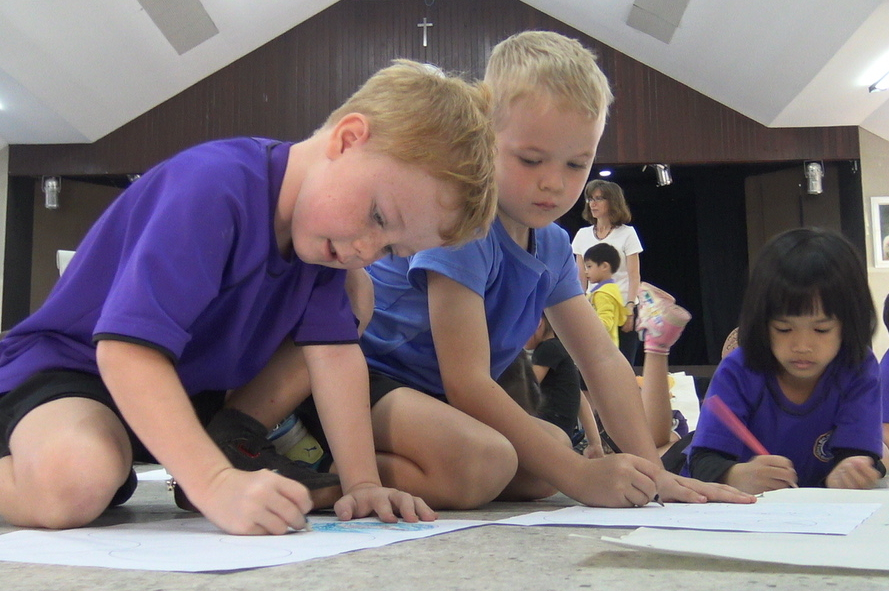
\includegraphics[width=\textwidth]{chapter4_B3_p1.JPG}}

\minor{Formative Assessment Data}

Since 2014, formative assessment continues to play a central role in measuring student progress. Through formal and informal professional development (November 2014, January 2015, August 2016), CMIS Teaching Staff has developed a deeper, more conceptual understanding of formative assessment’s purpose, frequency, and relationship to grading and instruction. See \href{https://docs.google.com/document/d/1a7yAmVFIAjZcKHqivOLhF-RYoxJitoF7buq27Ck9sZM/edit?usp=sharing}{CMIS Formative Assessment Research Base} for a detailed definition of formative assessment use at CMIS. See CMIS Professional Development Action Plan for professional development on formative assessment. 

The \href{https://docs.google.com/a/cmis.ac.th/spreadsheets/d/1ACz3l3DPUgIqRhmZ1LWk9RwVBjo0iLsbJAupJoic5Dg/edit?usp=sharing}{Teach for Success Observational Protocol}, and instructional rounds, a two-month snapshot of assessment practices indicates that formative assessment is used regularly and monitoring and adjusting instruction are used consistently. 

\href{https://docs.google.com/a/cmis.ac.th/document/d/1cRvL50iIDvo8s1Gnxoczm82LhSVmEOvCrFksxzHD7ko/edit?usp=sharing}{Teach for Success data} indicated that formative assessment was used 8 times out of 36 observations. Though this seems like a low percentage (22\%), teachers who were observed utilizing formative assessment accomplished the entire formative cycle: by providing immediate feedback, involving the learner, and using the results to inform their instruction. This is usually difficult to observe during one learning segment observation. 

{\centering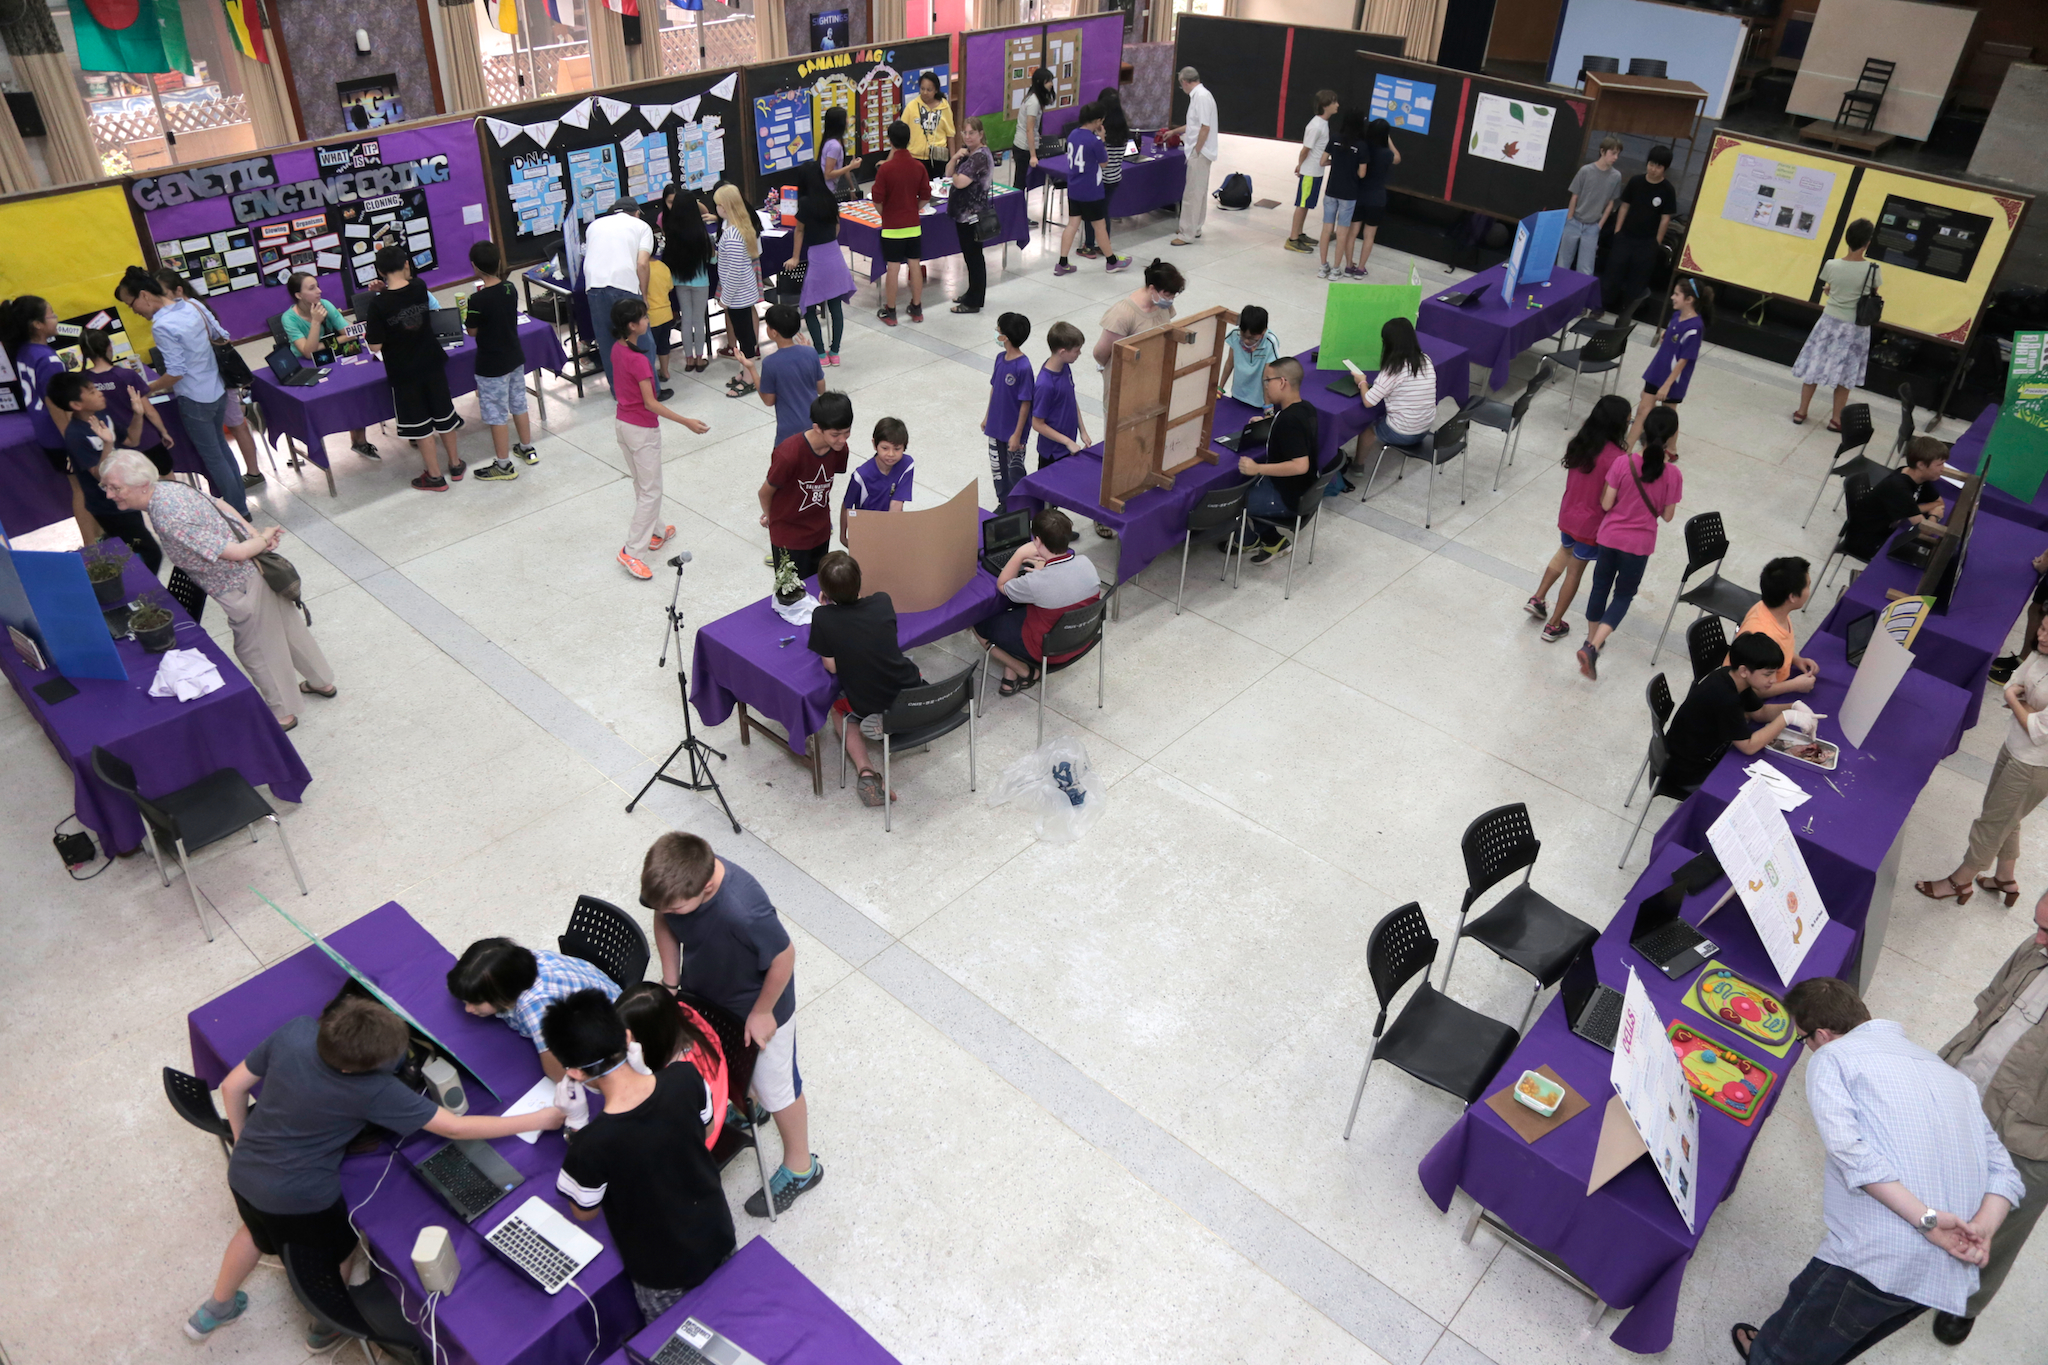
\includegraphics[width=\textwidth]{4_2_1_ha_b.jpg}} 

Teacher-to-teacher interviews, corroborated by administrative walk throughs, formal evaluations, and instructional rounds, provided a wealth of information about the formative assessment practices in the CMIS classroom. A representative sample of responses found strong alignment between the CMIS Teaching Staff use of formative assessment and the attributes of quality, formative assessment found in the Formative Assessment Research Base. Teachers stated that they use formative assessment to:

``...reassess a unit plan and make adjustments for future lessons''
``...provide instant feedback with Google Forms''
``...in music and PE, instant verbal feedback is used'' 
``...to focus on a learner centered problem [in Datawise] and step back a bit with a mini lesson to address the problem.'' 
``...provide detailed information on individual achievement and the grouping of students''
``...[assess effectiveness of the test by] changing a question or taking out a question''
``...reteach concepts''
``...rewrite unit plans, this happens all of the time. You think they’ve got something, but they don’t.'' 
``...[for] sight words, student struggles and I adjust instruction.''
``...quiz scores indicated low comprehension assigned materials; adjusted by providing a teacher made reading guide.''
``...[use as] a preassessment and I base units on results''

Though the CMIS Teaching Staff understand that it’s not the design of a test, technique, strategy, activity, or self-evaluation, per se, that makes it a formative, but the way it is used. There are a handful of strategies that most CMIS teachers use, including: exit slips, graphic organizers, quizzes, discussion protocols, and anecdotal notes. 

Additionally, since 2015, a formative assessment section was added to all teacher created Understanding by Design plans to continue to build capacity and understanding of formative assessment. Discussions that have arisen from this section of the UbD plan, in divisional and department gatherings, have provided valuable professional conversations. Please see the CMIS \href{https://docs.google.com/a/cmis.ac.th/document/d/1PsJDkNbtYw-tEd96wM6tFjMWQ2xNZaiwhJAbfQvlNxI/edit?usp=sharing}{UbD Template 3.0} and the \href{https://docs.google.com/a/cmis.ac.th/document/d/1kL1VjwfuMMa7NaWmwUrEah1BM-jJRmLAd4VJzR3HoPs/edit?usp=sharing}{UbD Menu} for more information. 

\minor{Monitoring and Adjusting Instruction}

At CMIS, monitoring and adjusting instruction is viewed as different from formative assessment. At CMIS, monitoring and adjusting is defined as:

When monitoring and/or adjusting individually or collectively, the teacher observes student progress during instructional time or during an activity, and makes appropriate adjustments in teaching, provides recognition or offers additional support, prompts, cues or assistance as needed. The teacher walks about, looks about, and talks to students regarding their progress. Monitoring learning and adjusting teaching or providing immediate assistance promotes correct learning (Hunter, 1982, Cotton, 2002, and Marzano, 2003). Teacher attributes of monitoring and adjusting include: 

\begin{itemize}
\item Observe student progress
\item Respond to student progress appropriately
\item Provide recognition or offers support, prompts, cues or assistance
\item Adjust teaching as needed
\end{itemize}

Using these attributes as indicators, over 90\% of the CMIS Teaching Staff used monitoring and adjusting during their instructional time between September and November, 2016. See \href{https://docs.google.com/a/cmis.ac.th/document/d/1cRvL50iIDvo8s1Gnxoczm82LhSVmEOvCrFksxzHD7ko/edit?usp=sharing}{Teach for Success Instructional Data}. 

\minor{Summative Assessment}

By becoming more familiar with formative assessment, the CMIS Teaching Staff also developed a deeper, more conceptual understanding of summative assessment’s purpose, frequency, and its relationship to grading and instruction.

{\centering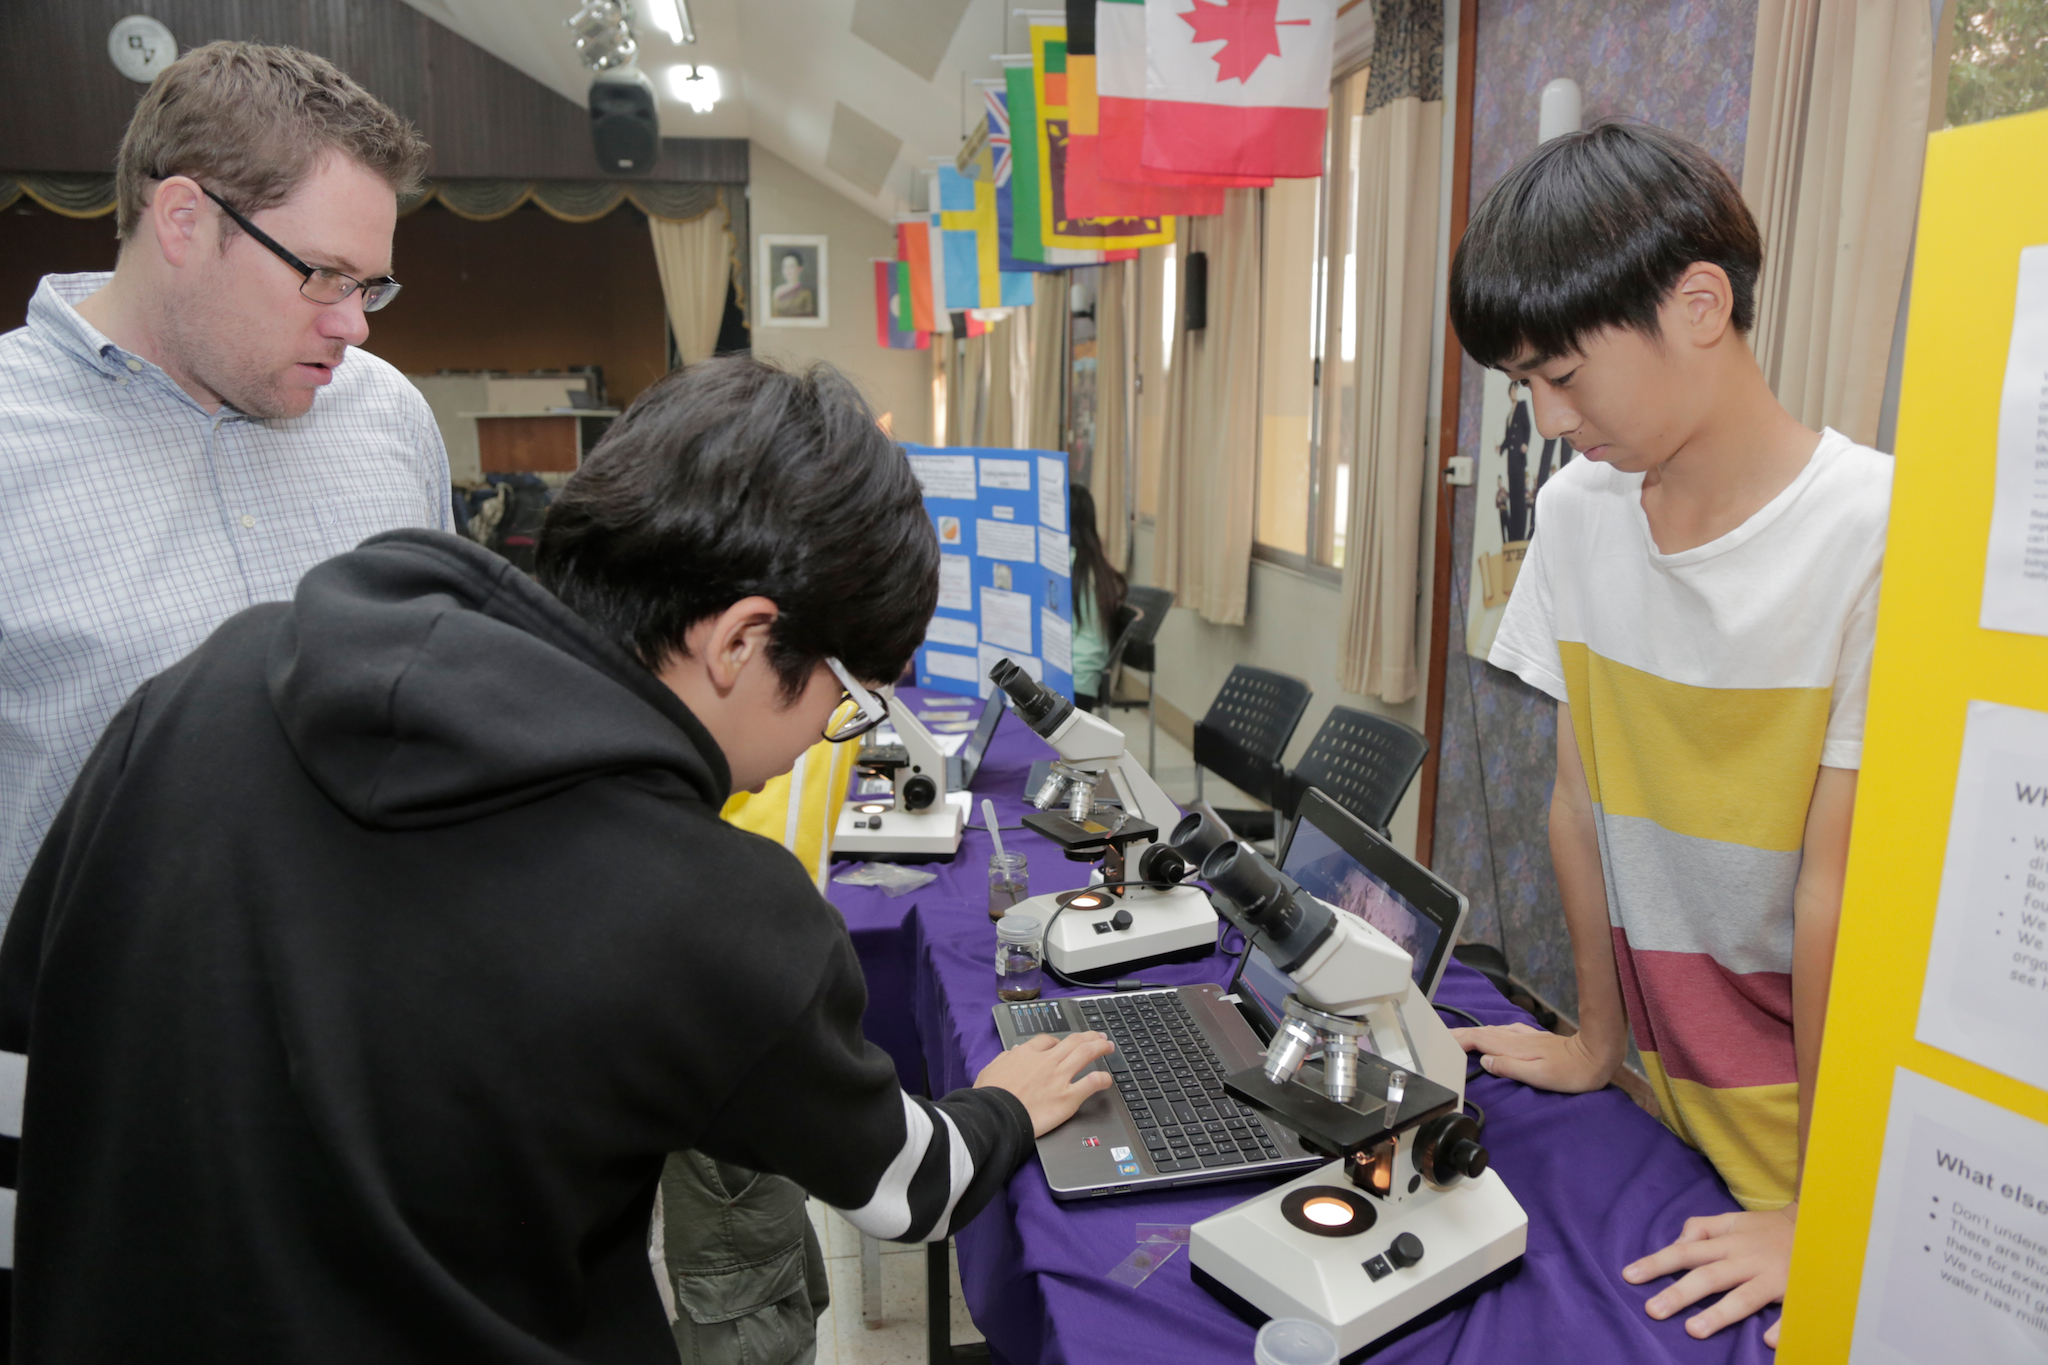
\includegraphics[width=\textwidth]{4_2_1_ha_a.jpg}}

At CMIS, summative assessments are used to evaluate student learning, skill acquisition, and academic achievement at the conclusion of a defined instructional period—typically at the end of a project, unit, course, semester, program, or school year. 

Generally speaking, summative assessments at CMIS are defined by three major criteria:

\begin{itemize}
\item The tests, assignments, or projects are used to determine whether students have learned what they were expected to learn. In other words, like formative assessment, what makes an assessment “summative” is not the design of the test, assignment, or self-evaluation, per se, but the way it is used—i.e., to determine whether and to what degree students have learned the material they have been taught.
\item Summative assessments are given at the conclusion of a specific instructional period, and therefore they are generally evaluative, rather than formative—i.e., they are more appropriately used to determine learning progress and achievement, evaluate the effectiveness of educational programs, measure progress toward improvement goals, or make course-placement decisions, among other possible applications.
\item Summative-assessment results are often recorded as scores or grades that are then factored into a student’s permanent academic record as letter grades on a report card or test scores used in the college-admissions process. 
\end{itemize}

The CMIS 9-12 Teaching Staff have paid special attention to summative assessments through the Summative Assessment (Final Exam) Peer-to-Peer Meetings. Though different protocols have been used to promote discussion in department level peer groups, all of these protocols have provided participants with a structure to ensure that everyone has opportunity to participate, limit unfocused participation, and, depending on the structure, build on previous professional development. 

{\centering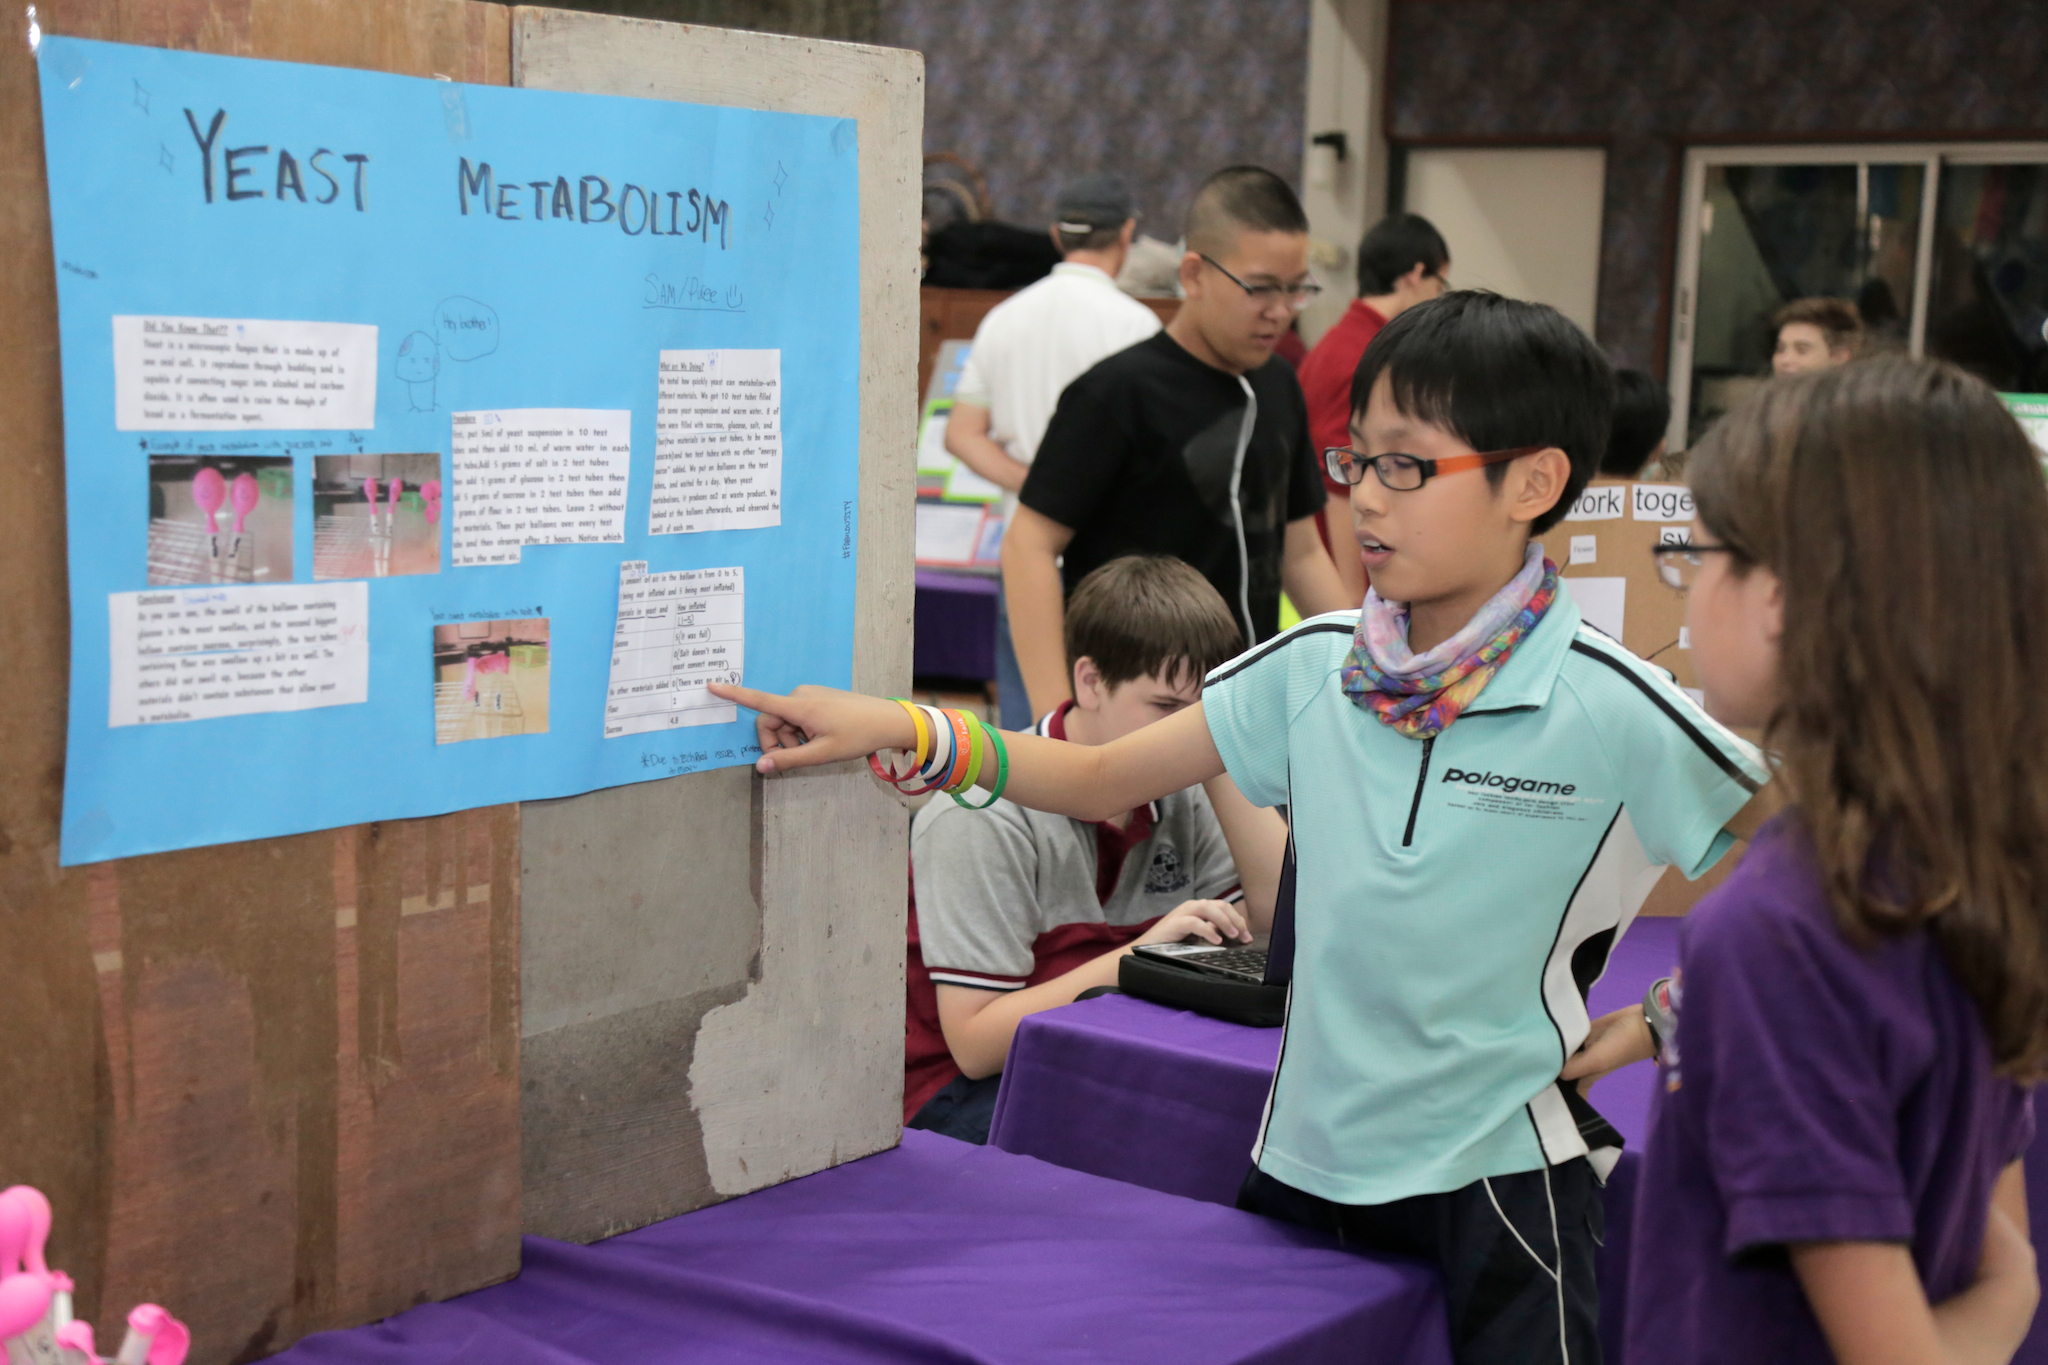
\includegraphics[width=\textwidth]{4_2_1_ha_c.jpg}}

Since 2014, the Peer-to-Peer Summative Assessment Meetings have used the following protocols:  warm/cool feedback, notices and wondering, Collaborative Assessment Conference. During these meetings, participants must bring a copy of their summative assessment along with the grading criteria and rubric along with their assessment blueprint. A requirement since 2014, the assessment blueprint outlines the aligned of each question to a standard and the Depth of Knowledge level. The blueprint is a tool help facilitate discussions on assessment alignment to the standards and if the question is at the level of complexity required by the standard.  Follow up with representative participants have indicated that many use the descriptive feedback provided during the meetings to improve their summative assessments. See Summative Assessment Peer Review: \href{https://drive.google.com/a/cmis.ac.th/folderview?id=0ByVFfrm0zfolTHY0dmtURG5pcGs&usp=sharing}{Fall 2014}, \href{https://drive.google.com/a/cmis.ac.th/folderview?id=0ByVFfrm0zfolaWQzeWxCTlVyUFU&usp=sharing}{Spring 2015}, \href{https://drive.google.com/a/cmis.ac.th/folderview?id=0ByVFfrm0zfolRjQzTDhmT0dyYzg&usp=sharing}{Fall 2015}, and \href{https://drive.google.com/a/cmis.ac.th/folderview?id=0ByVFfrm0zfolT29vQXpQeXp3VlU&usp=sharing}{Spring 2016} for more information. 

Though types and frequency of summative assessments vary depending on the grade level and content, the CMIS Teaching Staff use a number of assessments for summative outcomes; these include end unit tests, final and midterm tests, culminating products, and performance tasks. 

\minor{Standardized Testing}
 
CMIS Teaching Staff also use norm referenced, standardized summative assessments to measure curriculum effectiveness and student achievement. Traditionally, CMIS has used the International School Assessment (ISA) in grade 3, 5, and 7. ISA provided CMIS Leadership and Teaching Staff with important data such as comparison of like schools (program efficacy) and mathematical literacy, writing, and reading (student achievement). After a review during the 2016-2017 year, CMIS Leadership wanted to provide students, teachers, and the CMIS community with a standardized test that was more strongly aligned to our adopted standards. The Measures of Academic Progress (MAP) test produced by the Northwest Evaluation Association (NWEA) was vetted and implemented. Using the MAP test will provide CMIS with data that not only includes a comparison of like schools, but will also be aligned to our ELA and mathematics standards to help measure student achievement. The CMIS Leadership and Teaching Staff look forward to using the assessment data to continue our work with Datawise and evaluate program efficiency. 

Other criterion-referenced, standardized test used by CMIS are the Advanced Placement (AP) exam and the Preliminary Scholastic Aptitude Test (PSAT 8/9, PSAT NMSQT) and the Scholastic Aptitude Test (SAT).
  
\minor{Global Competency and Assessment}

CMIS does not provide stand alone assessments that include explicit questions about  the world, multiple perspectives, communicating ideas etc. If those competencies are found within these content standards,  disciplinary frameworks, or habits of mind, then those competencies will be assessed. Social studies, science, English, and math assessments have student questions that ask the students to consider global competencies. Additionally, many examples of authentic and performance assessments in all grade levels and all contents ask students to communicate ideas effectively, consider multiple perspectives, take action etc. 

\minor{So What...}

CMIS uses a variety of assessments to measure  student progress and achievement. As mentioned in the Planning Process indicator in the How Students Learn: CMIS has made significant strides in the understanding of formative assessment and a handful of teachers use the formative data skillfully and strategically. Data also indicates that formative assessment is used more frequently than in previous years. CMIS would benefit from time and resources used to train some teachers on transitioning from good formative assessment to great formative assessment. Good formative assessment is giving it and using the data to inform your (i.e. the teacher’s) future instruction. Great formative assessment is involving the students in the data results to make achievement for all students in all courses/grade levels a reality.
\end{findings}

\subsubsection{Basis for Determination of Performance Levels}

\indicator{The school staff has determined the basis upon which students’ grades and their growth and performance levels are determined and uses that information to strengthen high achievement of all students.}

\prompt{Evaluate the impact and effectiveness of the basis for which students’ grades, their growth, and performance levels are determined.}

\begin{findings}
The CMIS Teaching Staff use many different measures to determine both student grades and achievement. The Staff also uses assessment data to address student achievement. 

The bases for how traditional student grades (i.e. number codes in K-5, letter grades based on percentages in 6-12) are determined differ in the K-5 and 6-12 division. 

\minor{Context for Grades in Elementary School Division}
 
The elementary school division operates on a two-semester system. 

There are two reporting periods at the elementary school where report cards are sent home to families. In addition to report cards, there are mid-semester updates and Family-Teacher Conferences. A mid-semester update is shared in October, during our Family-Teacher Conferences for all students. First Semester Final Grades – are issued in December as part of each student’s annual Report Card. A mid-semester update is shared in March, during our Family-Teacher Conferences for all students. Second Semester Final Grades - are issued in June as part of each student’s annual Report Card.

CMIS Leadership strongly encourages teachers to contact parents if they feel that a student is struggling. CMIS Leadership and the Parent Teacher Group encourage parents to contact the teachers, counselors, or the administration any time they have concerns about their child, their progress, or anything to do with the class or school. It is not necessary for parents to wait for a grading period or Family Conference to contact a teacher. CMIS staff are available and are here to work in conjunction with parents to help our students succeed. Academic progress is assessed through a variety of ongoing assessments, and is reported informally through work sent home and notes in the student planner, and formally through report cards and family conferences.

{\centering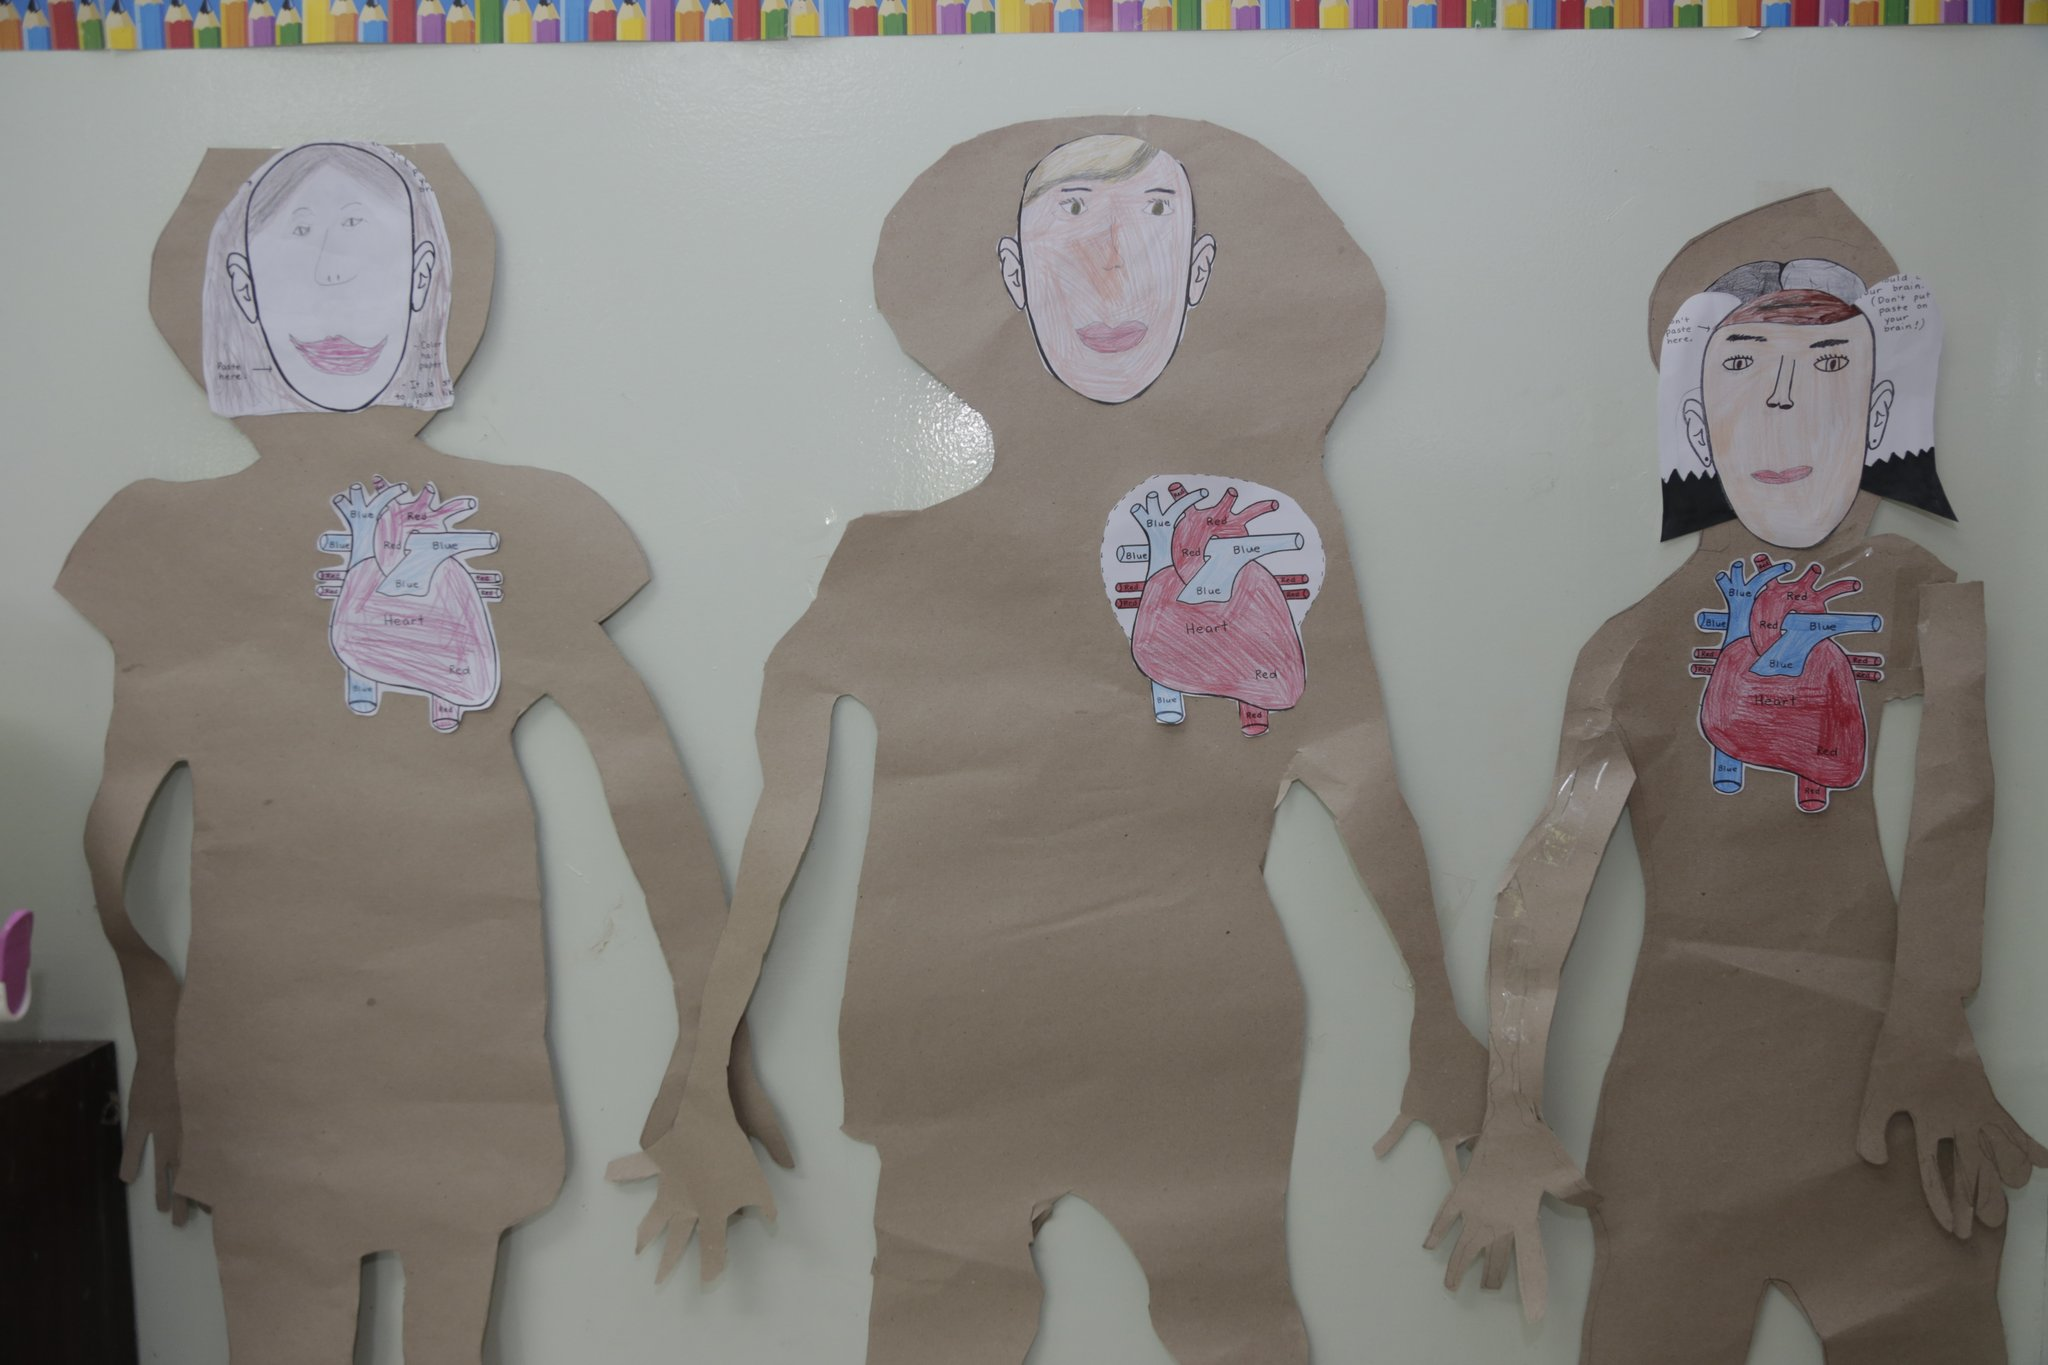
\includegraphics[width=\textwidth]{4_2_1_ha_d.jpg}}

All students from K-5 are assessed regularly by their teachers, formatively and summatively. These assessments provide evidence of achievement and also help teachers in their planning of future lessons. The CMIS report cards have two major sections for reporting this information achievement and effort. See the Grading section of \href{https://docs.google.com/document/d/1bIbV9pgGz2vpXYJdnRzL_Od5PS35egy7lgBOBuszgD4/edit#heading=h.2vxh95cg5cjg}{student handbook} for more information. 

\minor{Context for Grades in Middle/High School Division} 

Like the Elementary School division, the Middle and High School operate on a two-semester system. There are two main reporting periods on a student’s official school transcript; First Semester Final Grades (December) and the Second Semester Final Grades (June).

Like many schools, final grades are issued at the end of each semester, and become part of each student’s official transcript. Grade-to-date academic progress in all subject areas is available for viewing through the Powerschool online platform throughout the grading period. CMIS Leadership strongly encourages students and parents to access Powerschool on a regular basis to track student progress. CMIS Leadership provides two scheduled times for  Family-Teacher Conferences in October and March, but teachers are expected to contact parents if they feel that a student is struggling at any time of the year. Likewise, parents are encouraged to contact the teachers, counselors, or the administration any time they have concerns about their child, his/her progress, or anything to do with the class or school. CMIS Leadership emphasize that it is not necessary for parents to wait for a grading period or conference to contact a teacher. 

The CMIS Academic Standards are the baselines for grades and measurement of growth/performance levels. Each content has specific standards that are outcome focused, progressive, and rigorous. Achievement and letter percentage grades are determined using summative assessments (which include the use of performance tasks, checklists, and rubrics), as well as evaluated learning tasks and activities that are aligned to the academic standards.

CMIS uses multiple measures to determine student growth and performance levels. As mentioned previously, the CMIS Teaching Staff use rubrics, checklists, anecdotal notes, as well as traditional pencil/paper tests that incorporate selected response, short answer, multiple corrects, and essay questions. 

Efforts have been made to strengthen the alignment of the assessments to the adopted standards and to address the appropriate rigor of the assessment questions, especially in grades 9-12. As addressed in the Professional Collaboration sections, other strategies are used to examine assessment to improve learning and address student achievement. These structures include:

\begin{itemize}
\item Inter-rater reliability-used on numerous occasions to ensure reliability in grading (e.g., common argumentative rubric meetings) and in unit construction (e.g., UbD Interrater meeting) 
\item Peer review-used consistently for the CMIS Summative Assessment/Final Exam feedback meetings organized once a semester. Protocols became more structured as time progressed. 
\item Depth of Knowledge (DOK)- Focuses on complexity of content standards, assessment items, or instructional tasks The outcome (product) is the focus of the depth of understanding. Training began in Fall, 2016 and continues throughout the year.
\end{itemize} 

Finally, a number of diagnostic assessments are used to ensure appropriate intervention and/or placement of students. The Developmental Reading Assessment (DRA), WIDA Access Placement Test, and the admission placement assessment are all examples of diagnostic assessments used by the CMIS Teaching staff. 

\minor{So What...}

As in the Student Understanding of Performance Levels section: Data indicate that students equate performance levels with letter grades. When interviewed about how their grades are determined, a vast majority of students state that the grade is based on homework, activities, tests, labs, and projects--though this is accurate, they have less awareness of performance levels based upon rubrics and formative assessment. CMIS should continue to implement the posting or verbally stating of the objective and or standards to increase student understanding of their class or course performance levels and standards. The CMIS Teaching Staff could encourage this by providing opportunities for students to demonstrate understanding beyond letter grades and/or percentages.
\end{findings}

\subsubsection{Demonstration of Student Achievement}

\indicator{A range of examples of student work and other assessments demonstrate student achievement of the academic standards and the schoolwide learner outcomes, including those with special needs.}

\prompt{Examine and evaluate how student work and other assessments demonstrate student achievement of the academic standards and the schoolwide learner outcomes.}

\begin{findings}
As mentioned in the Student Work- Engagement in Learning section, the CMIS Teaching Staff have used a number of protocols to help structure a discussion that focuses on student achievement and alignment to academic standards. CMIS Teachers look at student work to make informed instructional decisions and use as a basis for discussions about alignment to standards and schoolwide learner outcomes. Discussion about academic coherence, focus, and rigor also are generated from these opportunities. 

CMIS Leadership has implemented research-based instruments to examine student work to ensure  alignment to student learner outcomes and CMIS standards; also to ensure effective collaboration. 

\minor{Summative Assessment Peer Review}

Peer review is used consistently for the CMIS Summative Assessment/Final Exam feedback meetings, which are organized once a semester. Protocols became more structured as time progressed.

\minor{Looking at Student Work}

CMIS Teaching Staff have used the adapted \href{https://docs.google.com/a/cmis.ac.th/document/d/1aobA3IksQDoGJ-JKci0YDfFDCgT2ugHM7r_T4i_CL7o/edit?usp=sharing}{Longfellow Slice} as well as CMIS teacher created protocol-called the CMIS Slice (in development). CMIS Leadership uses norms from National School Reform Faculty and \href{https://drive.google.com/a/cmis.ac.th/file/d/0ByVFfrm0zfoleTBsYnhNUFZHbVE/view?usp=sharing}{Annenberg Learner’s Critical Friends Group}. Student Learner Outcomes were also examined in context of examining student work. See the \href{https://docs.google.com/a/cmis.ac.th/document/d/1En9qeldzNSJDHs7m_jRRqNUx6v1EMKD_5MRH0GJsFQM/edit?usp=sharing}{Purpose of the Longfellow Slice} for more information. 

\minor{So what...}

Though CMIS has initiated resources and times for looking at student work, the CMIS Teaching Staff would like to continue to focus on it with more regularity and with a different focus each session  (i.e. progression, coherence, rigor etc.). Consistent analysis of student work and assessments will provide data on  student achievement of the academic standards and the schoolwide learner outcomes.
\end{findings}

\subsubsection{Correlation}

\indicator{The teachers correlate assessment to schoolwide learner outcomes, academic standards, course competencies, and instructional approaches used.}

\prompt{Comment on the correlation of assessment of schoolwide learner outcomes, academic standards, course competencies, and instructional approaches used.}

\begin{findings}
See Demonstration of Student Achievement 
\end{findings}

\subsubsection{Modifications/Decisions based on Assessment Data}

\indicator{Assessment data is collected and analyzed and used to make changes and decisions about curriculum, instruction, professional development activities, and resource allocation. Teachers modify and revise the curriculum and instruction as a result of student assessment, both collectively and individually.}

\prompt{Evaluate the effectiveness of how assessment data is collected, analyzed, and used to make changes and decisions about curriculum, instruction, professional development activities, and resource allocation.}

\begin{findings}
Assessment data is used consistently by the CMIS Teaching Staff and Leadership to make curriculum/resource, instructional, and professional development. 

\minor{Data for Curriculum/Resources}

All curriculum and adoption decisions are based on the \href{https://docs.google.com/a/cmis.ac.th/document/d/1hh1nLUlJgg1hd7s6aG3u3We0L6o7Wg_ECdjc2f6DcT8/edit?usp=sharing}{Curriculum Resource Adoption Cycle}. The adoption of curriculum/resources is a multiple-month process that entails teams of teachers who are provided time, usually during the school day, for professional development on:

\begin{itemize}
\item The standards and the necessary instructional shifts they require. 
\item The research-based vetting instruments. 
\end{itemize}

As it is widely understood that: 

Evaluating instructional materials requires both subject-matter and pedagogical expertise. Evaluators should be well versed in the Standards for all grades in which materials are being evaluated. This includes understanding not only the individual standards statements, but also the overall structure of the standards itself, as well as the expectations of the Standards with respect to conceptual understanding, procedural skill and fluency, and application.

One half of the CMIS Adoption Process involves unpacking and working with the standards.
                                  
The CMIS Adoption Process begins with a \href{https://goo.gl/forms/wV2k8Nef218a8Tcq2}{needs assessment} which asks teachers to reflect on the current curriculum and resources CMIS currently utilizes in that particular content and the gaps in curriculum. Using this data as a starting point, teams of teachers use the vetting instruments to ensure that all resources and curriculum purchases are:

\begin{itemize}
\item Aligned to the CMIS Standards (including essential shifts required by some standards)
\item Engaging- provides teachers with structures that allow students to use inquiry, speaking and listening, and/or differentiation. 
\item Rigorous- though the rigor resides in the standards, the vetting instruments ensure that a range of complexity levels (DOK) are embedded in the program and that it does not encourage instructional practices that are not research-based. 
\end{itemize}

Final decisions for purchasing are based upon the data from the vetting instruments, which are made up of research-based rubrics with a scoring criteria. The 2015-2016 school year focused on science adoption. Discussions with teacher teams and the needs assessment data revealed that science teachers in grades 6-12 used multiple online resources that were mostly vetted for NGSS alignment, engagement, and rigor, so it was decided that they will not purchase publisher-created curriculum and resources. Data from teachers in grades K-5 revealed a different set of needs. Through analysis of the needs assessment and discussion with teacher teams, teachers in grades K-5 needed a much more structured science program.  Though appropriately certified and qualified, none of our K-5 teachers had a background in science, so vetting and purchasing a publisher-based science program was not only appropriate, but necessary as it would provide teachers with accurate content knowledge and practices that would align to the critical shifts in their new science standards. 

{\centering\includegraphics[width=\textwidth]{4_2_1_ha_e.jpg}}

Mathematics for grades K-12 went through the same process during the 2016-2017. Social studies/ELA are planned for the adoption process during the 2017-2018 year. 

The CMIS Adoption Cycle and Process was created to ensure that CMIS purchases quality resources for major adoptions. As with other schools, CMIS does have to purchase smaller orders of curriculum and resources. These are usually on increased class sizes, replacement of damaged resources, addition of courses to the catalog. In order to ensure the same high quality purchases, a Resource Request and Resource Renewal process was created. For convenience, each request is an online Google Form; teachers respond to brief questions about the extent the resource aligns to standards and addresses student achievement.

\minor{Data for Instructional Decisions}

Observational and survey data indicate that the CMIS Teaching Staff use assessment data to make adjustments and modifications to instruction consistently. 

Instructional rounds, conducted between September and November indicate that over 95\% of the instruction was monitored and adjusted during the observational period. 
 
In order for this to be observed, individually and/or collectively, the teacher must observe student progress during instructional time or during an activity, and make appropriate adjustments in teaching, as well as provide recognition or offer additional support, prompts, cues or assistance as needed. Monitoring learning and adjusting teaching or providing immediate assistance promotes correct learning (Hunter, 1982, Cotton, 2002, and Marzano, 2003). The following attributes had to be observed by the participants: 

\begin{itemize}
\item Observes student progress
\item Responds to student progress appropriately
\item Provides recognition or offers support, prompts, cues or assistance
\item Adjusts teaching as needed
\end{itemize}

Monitoring and adjusting during this period could be classified into three categories: circulating among students and responding to and asking questions, impromptu working with small groups or individual students to assist, and “pausing” instruction to adjust. See \href{https://docs.google.com/a/cmis.ac.th/document/d/1cRvL50iIDvo8s1Gnxoczm82LhSVmEOvCrFksxzHD7ko/edit?usp=sharing}{Teach for Success Data} for more information. 

Survey data also suggests CMIS teachers consistently collect data to make instructional decisions. A representative sample of responses include:

``I use pretests and prewrites to see where the students are starting'' 
``I rewrote a quiz because of poor results and started from there''
``I adjusted instruction and reviewed my activities with sight words. I tried internet-based resources and hands on approaches''
``I often do that in math, not ready to progress until mastery is achieved. A new lesson or method [is what I] most frequently [use]''
``Last year I realized none of the elementary kids could skip, so I added it into my instruction on a regular basis.''
``On multiple occasions on observational data I have to back up and teach prerequisite skills that they didn’t have'' 
``Online multiple choice quizzes help assess if students can move or if they all need to review''

Because analyzing and using assessment data to make changes and decisions about instruction is also the definition of formative assessment, see Appropriate Assessment Strategies section for more teacher examples of the practice. 

Please see section entitled Challenging and Varied Instructional Strategies for more detailed data about how instructional data is used.

\minor{\href{https://docs.google.com/a/cmis.ac.th/presentation/d/1omzyjfwf5fazGCSuvw7dDQn4eqhpOIaldeLXY7-6PYQ/edit?usp=sharing}{Datawise}}

As mentioned in the section entitled Congruence, CMIS Leadership and Teaching Staff have implemented the Datawise Process. Using this process, CMIS has created school data teams of teachers and administrators who make use of performance data and other information to target educational questions to pursue, identify major gaps in student understanding, identify target areas called learner-centered problems (LCP), reframe learner-centered problems as problems of practice (POP), target solutions to problems of practice, and write action plans pinpointing solutions. 

CMIS Leadership and Teaching Staff used 2014-2015 ISA data to develop a CMIS specific schoolwide LCP, created a schoolwide POP, each department created a strategy to address the POP, and assessed throughout the 2015-2016. Based upon teacher feedback and achievement data, the 2016-2017 year Datawise program was modified to allow each department to determine their LCP and POP based upon department specific data. The departments’ Datawise plan is currently being implemented. By using the Datawise process, the CMIS Leadership Team and Teaching Staff have ensured academic outcomes (i.e. standardized test data) are used to make instructional decisions that are based upon students’ skills/concepts, and the academic standards. 

\minor{Data for Professional Development}

\href{https://docs.google.com/a/cmis.ac.th/document/d/1cRvL50iIDvo8s1Gnxoczm82LhSVmEOvCrFksxzHD7ko/edit?usp=sharing}{Instructional Rounds data} will be used for elements of future professional development decisions in the future. One of the strengths of the Rounds process is asking teachers to reflect on their own practice and create a personalized focus question to help guide the other members of the Rounds group in their data collection tasks. The focus question must relate to instruction or assessment and must be answered by data collection. This focus question is sometimes called a deliberate practice and is one that teachers would like to continue to learn more about. In analyzing the focus question data,  55\% of the teachers developed a question about engagement. For example, are my students engaged? Or, how many of my students are engaged? Or, when I am doing small groups, are the other students engaged? 20\% of the questions dealt with assessment, like Do my students understand the content? And, How do I check for understanding? Finally, 10\% centered on standards and objectives, such as Am I communicating the objective effectively? And, How do I communicate in my class? CMIS Teaching Staff will use the Instructional Rounds focus question as the nexus of professional improvement and professional development. CMIS will continue to encourage professional development that is grounded in data individually (Instructional Rounds) or collectively (Datawise). 

\minor{So what...}

CMIS uses data to make decisions about curriculum, instruction, professional development, and resources. CMIS Leadership will monitor and maintain these  processes. As mentioned in previous sections, CMIS would gain additional  
\end{findings}

\subsubsection{Student Feedback}

\indicator{Student feedback is an important part of monitoring student progress over time based on the schoolwide learner outcomes and the curricular objectives.}

\prompt{To what extent is student feedback an important part of monitoring student progress over time based on the schoolwide learner outcomes and the curricular standards?}

\begin{findings}
The CMIS Teaching Staff elicit and use student feedback regularly. For findings in greater detail about formative assessment, please refer to sections entitled: Planning Processes, Professional Development, and Students Needs. Student feedback at CMIS can be categorized in the following ways:

\minor{Powerschool and Elementary Report Cards}

For grades 6 through 12, Powerschool is a secure web-based student management system designed to strengthen communication between the school and home by providing parents and legal guardians immediate access to their child's attendance records and academic progress online. Data indicate that teachers update student progress in terms of activity, assignment grades/completion, summative assessments, and in some cases, formative assessments on Powerschool regularly--at least once a week. This provides students an opportunity to monitor their own progress and parents to monitor their child’s progress. 

The elementary school teachers provide students and parents with report cards that indicate:
\begin{enumerate}
\item  Working Above Expectations
\item  Meeting Expectations
\item  Working Towards Expectations
\item  Working Below Expectations
\end{enumerate}

The CMIS Teaching Staff  use other methods to provide feedback, including comments in the grade book, on student work, and email communication home. Observational and interview data also indicate that the CMIS Teaching Staff also when possible return an assessment or activity as soon as possible (i.e. the next school day), provide immediate right/wrong (e.g., Kahoot, Socrative, LinguaFranca etc.), and immediate oral responses, especially in music and physical education. 

\minor{Formative, teacher-created feedback}

To the CMIS Teaching Staff and Leadership, providing students with quality, teacher-created feedback has the most impact on student achievement. Like John Hattie, CMIS believes that “The most powerful single modification that enhances achievement is feedback. The simplest prescription for improving education must be “dollops of feedback” (1992). Teacher-student feedback at CMIS can be organized into three categories:

\begin{description}
\item [Criterion referenced] Though they might differ in frequency and quality, all CMIS teachers use  rubrics at varying levels of frequency to assist in providing feedback. 
\item [Feedback for specific types of knowledge and skills] the instructional rounds process revealed that feedback is a practice with a high frequency. Between September and November, 2016 over 90\% of the instruction observed, some kind of specific feedback was provided to students either individually or collectively. Typically this type of feedback sounded like the following:
\begin{itemize}
\item ``good, looks like most of you…'' (MS science)
\item ``What do you think I’m going to say next…?'' (MS PE)
\item ``I think you should read this first…'' (HS PE)
\item ``...right, what would your next sentence be then?'' (HS math)
\item ``...have you thought about what your next step would be?'' (MS math)
\item ``...we need that to be a little sharper, okay let’s do that again'' (HS band)
\item ``...that’s probably why it's squeaking (recorder)'' (ES music)
\item ``...you need to make come from your stomach'' (MS drama)
\item ``...that’s right, now say it again.'' (ES ELA)
\end{itemize}

\end{description}

     
\minor{Student led feedback/self reflection}
 
Teacher interviews and survey data indicate that a majority of CMIS teachers provide consistent opportunities a year for students to lead their own feedback activity or self reflect. The following examples reflect this process: 

\begin{itemize}
\item Elementary PE teacher using laminated stars to ask student to reflect on their level of engagement for the period by counting starts-- student counted up to five stars together, five out of five was considered high engagement. 
\item High school ELA teacher provides his students with a peer review handout to help focus them when they pair up and peer edit each other’s writing
\item Middle school teacher asks her student groups to evaluate how well they worked in the group together. Feedback was only shared with student in the same group. 
\item High school science teacher provides students with a Google Document which allows collaboration and peer feedback to be completed synchronistically. 
\item High school social studies teacher provides time for his students to share +/- after student presentations. 
\end{itemize}

\minor{So what...}

As mentioned in the previous section: CMIS has made significant strides in the understanding of formative assessment and a handful of teachers use the formative data skillfully and strategically. Data also indicates that formative assessment is used more frequently than in previous years. CMIS would benefit from time and resources used to train some teachers on transitioning from good formative assessment to great formative assessment. Good formative assessment is giving it and using the data to inform your (i.e. the teacher’s) future instruction. Great formative assessment is involving the students in the data results to make achievement for all students in all courses/grade levels a reality. Additionally, planning processes should be designed with an emphasis on global competencies and the schoolwide learner outcomes more explicitly. 
\end{findings}

\subsubsection{Teacher Monitoring}

\indicator{Teachers monitor student progress over time and use student feedback as appropriate to determine whether course objectives and standards have been met.}

\prompt{Evaluate the effectiveness of the teacher monitoring process over time and the use of student feedback as appropriate to determine whether academic standards have been met.}

\begin{findings}
CMIS teachers monitor their student’s progress over time and use student feedback to determine if course objectives and standards have been met. 

As mentioned in the prior section, in grades 6 through 12, the Powerschool online platform provides students and parents the opportunity to monitor student progress, especially grades and/or assignment completion. In grades K-5, teacher-created report cards are the primary, formal means of monitoring student progress to the standards and objectives. This division also uses parent conferences, student planners, and are currently piloting electronic report cards to facillitate more efficient monitoring. 

The CMIS Teaching Staff use other, more effective, means to monitoring student progress. At CMIS, monitoring can be organized into three categories:

\begin{description}
\item [Small group] this monitoring strategy involves the teacher working in student groups of three to four to provide more focused instruction. Though usually used  as an intervention, data indicate that the CMIS Elementary Teaching staff use small groups to check for progress with an ongoing concept and provide targeted instruction for a new concept. Some other small group structures observed at CMIS include: small group discussions using a protocol, synchronistic- online discussions, silent discussions. 
\item [Individual] data suggest that the CMIS Teaching Staff use a variety of individual monitoring strategies, including: teacher/student and teacher/parent/student  conferences and taking anecdotal notes on individual students. Progress monitoring is also a systematic part of of our DRA reading inventory. 
\item [Collective] this monitoring type is the most used by the CMIS Teaching Staff. Collective monitoring, like formative assessment described in the previous indicators, take on many forms. The CMIS Teaching Staff use their formative assessments to monitor student progress, share with with students (so they can self monitor), and make necessary modifications to instruction. As was mentioned in Appropriate Assessment Strategies section, what makes an assessment “formative” is not the design of a test, technique, strategy, activity, or self-evaluation, per se, but the way it is used. Though that said, data indicate that the CMIS Teaching Staff use paper/pencil quizzes, exit tickets, oral-whole group assessments, whiteboards, online resources (e.g., Kahoot, Plickers, Socrative, Google Forms), and quick writes to monitor student progress collectively.
\end{description}
 
{\centering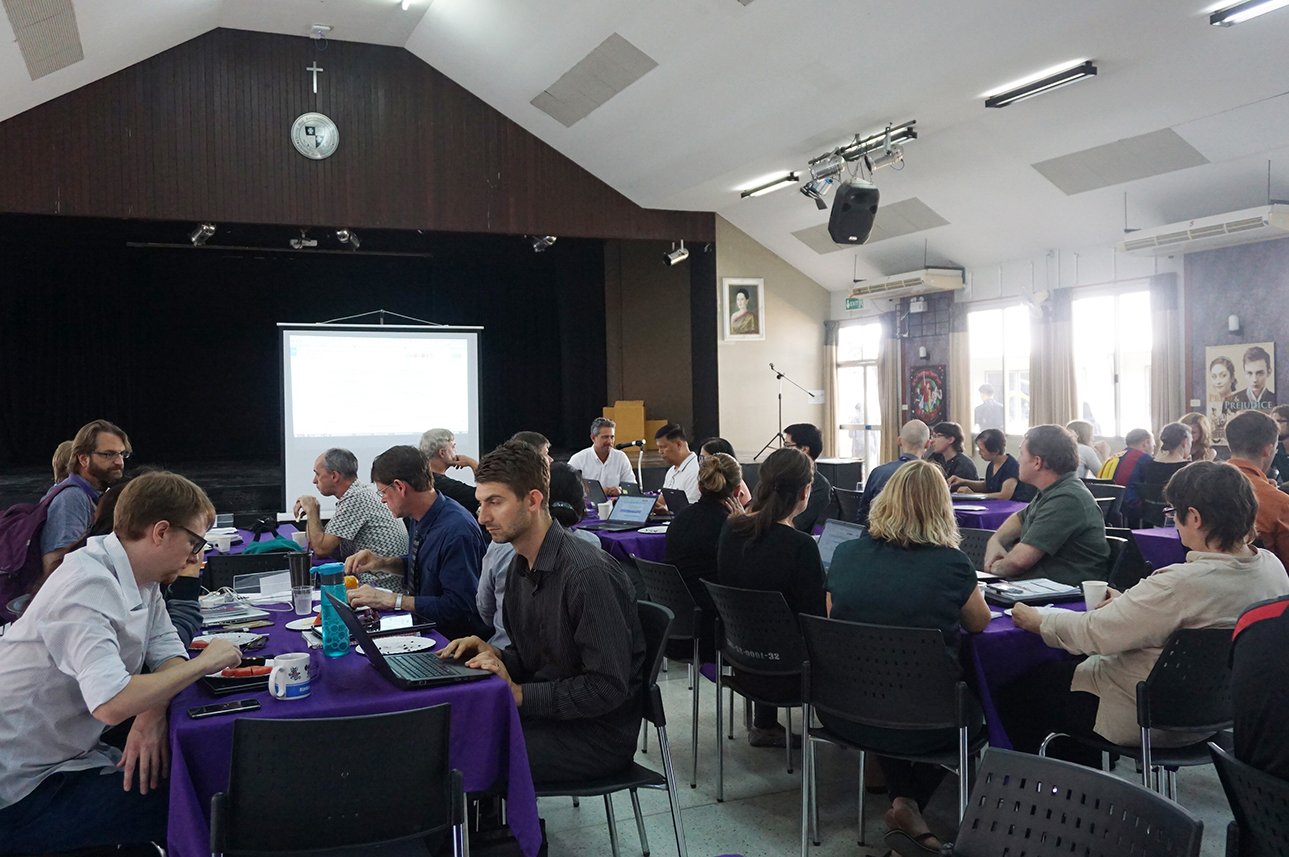
\includegraphics[width=\textwidth]{chapter4_B3_p2.JPG}}

\minor{So what...}

CMIS will continue to implement the effective use of formative assessment and will maintain the level of feedback CMIS Teachers provide students. As mentioned in prior sections, CMIS would benefit from time and resources used to train some teachers on transitioning from good formative assessment to great formative assessment. Good formative assessment is giving it and using the data to inform your (i.e., the teacher’s) future instruction. Great formative assessment is involving the students in the data results to make achievement for all students in all courses/grade levels a reality.

{\centering
\includegraphics[width=\textwidth]{4_2_1_ha_f.jpg}}

Additionally, data indicate that the use of small groups based on formative assessment results is rare in the middle and high school classes. Middle and high school students would benefit from more small group instruction based on formative assessment results for intervention or enrichment. Data suggest that a majority of instruction in high school is whole group. 
\end{findings}

\subsubsection{Conclusions}
\prompt{Comment on the degree to which this criterion is being addressed.}

\begin{findings}
The data indicate that CMIS addresses this criteria to a high degree. Every school can improve their assessment practices. Assessment research is constantly evolving and CMIS will continue to utilize research-based assessment practices. 

\minor{Maintain and Monitor}
\begin{itemize}
\item Continued and sustained use of formative assessment data by teachers and students to make instructional decisions.
\item Continued and consistent emphasis on looking at student work. 
\item Continue formative assessment discussions (e.g., what it is, how to use it) These have become common in many department and divisional meetings. CMIS will continue to focus on using formative assessment effectively. 
\item Continue work on standard alignment to assessments. This has been a priority for the past three years and will continue to be a focus for departments and divisions. 
\item Continue to provide opportunities for students using feedback to track progress.
\item Continue to emphasize academic standards as the appropriate baseline to monitor student progress.
\item Continue monitoring through Powerschool platform, small groups, individual, and collective structures. 
\end{itemize}

\minor{Continue to Improve}
\begin{itemize}
\item Continue the use and effectiveness of formative assessment. 
\item Continue to align teacher-created summative assessment to research-based, best practices. Expand summative assessment analysis to elementary division. 
\item Continue to emphasize looking at student work to demonstrate student achievement and alignment to standards. 
\end{itemize}
\end{findings}
